\bookpart{图结构与结构计算}{Graph Structure and Computation}
\label{part:graph-structure-computation}
\label{part:graphs}
\label{part:discrete-mathematics-and-graph-theory}

\BookPartGuide{%
道路网、任务依赖、人员与岗位的配对，都涉及有限个对象之间的直接连接。图用顶点表示对象，用边记录直接连接；方向、边权和属性再分别补充先后、数值和附加数据。本卷围绕这类对象展开四个部分：本部分建立图的结构并把结构算出来，第~\ref{part:graph-combinatorial-optimization}部分在给定边权与约束下选择最优的路径、生成树、流和匹配，第~\ref{part:set-functions-subset-selection}部分把选择对象推广为一般有限集的子集，第~\ref{part:graph-dynamic-programming}部分在图的分解上组织局部函数的动态规划。

本部分的两章分别回答“结构是什么”和“结构怎样算”。第~\ref{chap:graph-objects}章定义行走与路径、连通分量、强连通与弱连通、分隔集、树与生成树，比较边列表、邻接表、邻接矩阵和关联矩阵四种表示，并用同构区分结构差异与单纯改名。这一章的例子都小到可以手工核对，每个概念都配有核对给定结果的方法。第~\ref{chap:graph-traversal}章以邻接表为输入，用广度优先遍历和深度优先遍历在与顶点数加边数成正比的时间内求出最少边数、连通分量、强连通分量、拓扑序，以及删除给定分隔集后得到的局部块，再用顶点标记细化比较两张图的结构。

第~\ref{chap:graph-traversal}章的每个算法都输出第~\ref{chap:graph-objects}章定义的对象，所以前一章的定义与核对方法也是检验算法输出的标准。阅读时要注意三组区分。第一，结构上的连接与边上的数值不同：本部分只问能否连接、按什么次序，最少边数不是最短长度，生成森林也不比较总权，带权的优化属于下一部分。第二，必要条件与充分判据不同：度数、分量数和标记计数等不变量可以证明两图不同构，却不能证明同构。第三，无向与有向不同：有向图的可达不对称，连通要分强弱两种，环与无环的判断也各有规则。

图上顶点和边的数值函数、拉普拉斯矩阵、图谱与图滤波不在本卷讨论。本部分只说明邻接矩阵与关联矩阵怎样记录连接，并用矩阵幂计数行走；以这些矩阵为基础的图上算子与谱方法，可参考\BookChapterRef{part:graph-signal-processing}{卷九第三部分“图信号处理”}。}

\chapter{图与连接结构}
\label{chap:graph-objects}
\label{chap:graph-paths}

城市之间修了哪些道路，一项工程里哪项任务必须等另一项完成，这类信息都由“有限个对象”和“对象之间的直接连接”组成。我们关心的往往不是某一条连接本身，而是由连接串起来的整体：从一座城市能否开车到达另一座，拆掉一座桥以后交通网会不会断成两片，一组任务能否排出不违反依赖的先后次序。回答这些问题之前，先要说清图记录了什么、没有记录什么。

本章用集合、关系与映射的语言建立图这一对象，并沿“一步连接—多步连接—整体结构”的顺序展开。第~\ref{sec:graph-basic-concepts}节规定图记录哪些连接，方向、边权和子图分别附加或取出什么信息。一步的连接首尾相接，得到第~\ref{sec:graph-adjacency-paths}节的行走、路径与可达关系。无向图中的可达关系是等价关系，第~\ref{sec:graph-connectivity-separation}节据此把顶点划分为连通分量，并考察删除顶点或边怎样切断连接。

切断连接的研究说明，环上的边删去后图仍然连通。所以用最少的边保持连通的结构没有环，这就是第~\ref{sec:graph-trees-forests}节的树：它的路径唯一，边数恰为顶点数减一。最后两节转向记录与比较。第~\ref{sec:graph-representations}节比较四种表示的访问代价，其中邻接矩阵把行走计数变成矩阵乘法；第~\ref{sec:graph-isomorphism}节用同构判断两张图是否只差一套顶点名称。全章用同一张四个顶点、五条边的小图作贯穿例子。

本章只建立定义、基本性质和对给定结果的核对方法，所用的例子都小到可以手工完成。在大图上系统地求出可达集、连通分量、生成树和拓扑次序，需要广度优先遍历与深度优先遍历等算法，这是第~\ref{chap:graph-traversal}章的任务。带权路径的最短成本和总成本最小的生成树，分别在第~\ref{chap:shortest-paths}章和第~\ref{chap:minimum-spanning-tree}章讨论。

\section{图的基本概念}
\label{sec:graph-basic-concepts}

道路网记录哪些城市之间有直达道路，任务清单记录哪项任务直接依赖哪项任务。两者都由有限个对象和对象之间成对的直接连接组成，图就是描述这类信息的数学对象。本节先给出最简单的无向图，再根据实际需要依次加入方向和数值，最后讨论怎样从一张图中取出一部分。

\subsection{图的定义}
\label{sec:graph-conn-definition}

同一张道路网可以画成很多样子：城市的位置可以挪动，道路可以画直或画弯，两条道路在纸上还可能交叉。要判断两幅画描述的是不是同一张网，先得说清哪些内容是数据，哪些只是画法。对于“能否直达”这个问题，数据只有两样：有哪些城市，哪些城市之间有直达道路。

\paragraph{顶点集与边集}
把每个对象记为一个顶点，把每一对有直接连接的对象记为一条边，就得到一张图。这里先考虑没有方向的连接，例如可以双向通行的道路。

\begin{definition}[图]
\label{def:graph-conn-graph}
设$V$是有限集合，$E$是由$V$中两个不同元素组成的无序对$\{i,j\}$的集合，称$\mathcal G=(V,E)$为一个（无向）\term{图}（graph）。$V$中的元素称为\term{顶点}（vertex），$E$中的元素称为\term{边}（edge）。若$\{i,j\}\in E$，称$i,j$是这条边的两个端点。
\end{definition}

记$n=|V|$为顶点数，$m=|E|$为边数。全章使用同一个例子：
\begin{equation}
V=\{1,2,3,4\},\qquad
E=\bigl\{\{1,2\},\{1,3\},\{2,3\},\{2,4\},\{3,4\}\bigr\},
\label{eq:graph-conn-running-graph}
\end{equation}
它有$n=4$个顶点、$m=5$条边，可以看成两个三角形$\{1,2,3\}$与$\{2,3,4\}$共用边$\{2,3\}$。四个顶点之间最多有$\binom42=6$条边，这里只缺$\{1,4\}$。

\paragraph{图相等的判断}
既然图只由$V$和$E$确定，比较两幅图时只需读出各自的顶点集，把每条线段写成由两个端点组成的无序对，再比较两个顶点集和两个边集。图~\ref{fig:graph-conn-running-drawings}的三幅画顶点位置、线段形状和交叉情况都不同，读出的集合却都是式\eqref{eq:graph-conn-running-graph}，因此是同一张图。读边时只看端点，所以画面上的交叉点不是顶点，线段的长短也不是边的长度。问题若需要长度、坐标这样的数值，必须另外给出，见第~\ref{sec:graph-conn-weights}小节。

\begin{figure}[!htb]
  \centering
  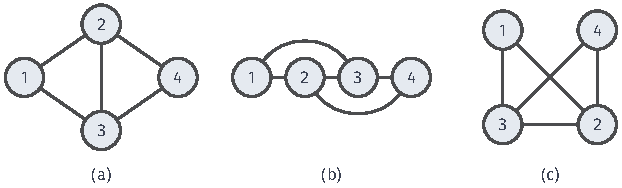
\includegraphics[width=106.765mm]{figures/01-basic-mathematics/04-graphs/tikz/c1-running-graph-drawings/figure.pdf}
  \caption{贯穿全章的四点五边图\eqref{eq:graph-conn-running-graph}的三种画法。顶点位置、线段形状和交叉情况都不同，但边集都是$\{1,2\},\{1,3\},\{2,3\},\{2,4\},\{3,4\}$。(c)中两条对角边在画面上交叉，交叉处不是顶点。}
  \label{fig:graph-conn-running-drawings}
\end{figure}

\paragraph{简单图}
定义~\ref{def:graph-conn-graph}要求边的两个端点不同，并且边集是普通集合，因此排除了一个顶点连到自身的\term{自环}（self-loop），也排除了同一对顶点之间的多条\term{平行边}（parallel edges）。满足这两条限制的图称为\term{简单图}（simple graph），本部分默认讨论有限简单图。简单图的每条边都是$V$的一个二元子集，而$n$元集合的二元子集共有$\binom n2$个，所以$m\leq\binom n2$。

如果两条平行道路需要分别记录收费，就得给每条边一个独立的身份，这时上面的边数上限也不再成立；用到这类扩展时会明确指出。另一个边界情形是顶点集为空的图。它只在少数论证中出现；结论需要至少一个顶点时，我们写明“非空图”。

\subsection{无向图与有向图}
\label{sec:graph-conn-directions}

道路可以双向通行，任务之间的依赖却有先后：“任务$i$完成后才能开始任务$j$”与“任务$j$完成后才能开始任务$i$”是两回事。无序对满足$\{i,j\}=\{j,i\}$，读不出谁在前。把每个依赖写成先做的任务在前的有序对$(i,j)$，次序就成了数据的一部分。

\begin{definition}[有向图]
\label{def:graph-conn-digraph}
设$V$是有限集合，$E\subseteq\{(i,j)\in V\times V:i\neq j\}$，称$\mathcal G=(V,E)$为\term{有向图}（directed graph）。有序对$(i,j)\in E$称为从$i$到$j$的\term{弧}（arc），也记作$i\to j$；$i$是它的起点，$j$是它的终点。
\end{definition}

为了区分，以无序对为边的图也称\term{无向图}（undirected graph）。有向图的弧集仍记作$E$，弧数仍记作$m$。弧$i\to j$只允许从$i$一步到达$j$，并不包含反向的$j\to i$。

图~\ref{fig:graph-conn-edge-vs-arcs}对照了无向边$\{u,v\}$与一对反向弧$(u,v),(v,u)$。两者都允许在$u,v$之间来回，区别在于无向边是一条连接，删除它就同时失去两个方向；两条弧是两个独立的对象，可以只删除其中一条，也可以分别附上不同的数值，例如上坡和下坡的用时。所以用一对反向弧代替每条边来改写无向图时，$m$条边变成了$2m$条弧，边的个数和身份都变了。

\begin{figure}[!htb]
  \centering
  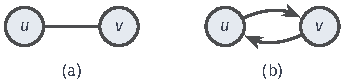
\includegraphics[width=62.974mm]{figures/01-basic-mathematics/04-graphs/tikz/c1-edge-vs-arcs/figure.pdf}
  \caption{一条无向边(a)与一对反向弧(b)都允许在$u,v$之间往返，但(b)中的两条弧是两个独立对象，可以分别删除或另附数值。}
  \label{fig:graph-conn-edge-vs-arcs}
\end{figure}

方向还决定了从哪里能走到哪里。图~\ref{fig:graph-conn-direction-orientation}给同一条三点连接1—2—3赋予不同的方向。不定向时，三个顶点两两可以互相到达；定向为$1\to2\to3$后，从$1$可以经$2$到达$3$，从$3$却哪里也去不了；定向为$1\to2\leftarrow3$后，$1$和$3$都只能到达$2$。

\begin{figure}[!htb]
  \centering
  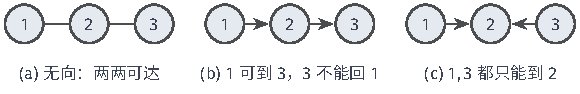
\includegraphics[width=98.189mm]{figures/01-basic-mathematics/04-graphs/tikz/c1-direction-orientation/figure.pdf}
  \caption{同一条三点连接的无向形式(a)与两种定向(b)(c)。箭头决定了从哪个顶点能走到哪个顶点。}
  \label{fig:graph-conn-direction-orientation}
\end{figure}

\paragraph{底层无向图}
有时只关心两个对象之间有没有直接联系，而不在乎谁先谁后。这时把每条弧$(i,j)$改写成无序对$\{i,j\}$放进一个新的边集；$(i,j)$与$(j,i)$同时出现时，集合中只留下一条边。得到的无向图称为原图的\term{底层无向图}（underlying undirected graph）。图~\ref{fig:graph-conn-direction-orientation}中(b)(c)的底层无向图都是(a)。这样做丢掉了先后：(a)中$3$能到达$1$，(b)中却不能，因此不能根据底层无向图断言原来的有向图可以双向到达。第~\ref{sec:graph-connectivity-separation}节定义弱连通时会用到底层无向图。

\subsection{边权与属性}
\label{sec:graph-conn-weights}

许多问题还需要每条连接上的一个数：道路有多长，管道每秒最多输送多少，两个样本有多相似。给定映射$w:E\to\mathbb R$，它在一条边$\{i,j\}$（或弧$(i,j)$）上的值称为\term{边权}（edge weight）；没有边的顶点对没有边权。

同一组边权在不同问题中参与的运算可以完全不同。图~\ref{fig:graph-conn-weight-semantics}在同一边集上附加同一组数，给出三种读法。读作长度$\ell_{i,j}$时，数值沿路线相加，路线$1,2,4$的总长是$2+1=3$，越小越好；读作容量$c_{i,j}$时，数值是单条边的流量上限，边$\{1,3\}$上至多通过$1$个单位，并不沿路线相加；读作相似度$w_{i,j}$时，权重越大，后续计算越强地要求两端的取值接近。所以拿到一张带权图，要先弄清权重的用途。

\begin{figure*}[!htb]
  \centering
  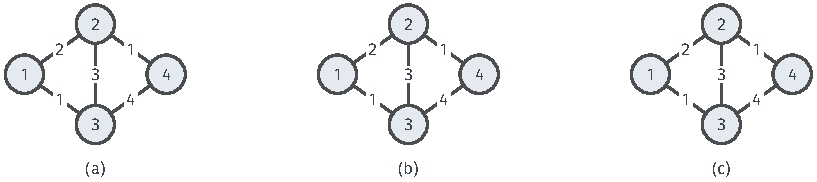
\includegraphics[width=138.187mm]{figures/01-basic-mathematics/04-graphs/tikz/c1-weight-semantics/figure.pdf}
  \caption{同一边集上的同一组边权在三种问题中的读法。(a)长度沿路线相加，路线$1,2,4$的总长为$3$；(b)容量限制单条边的通过量；(c)相似度越大，越要求两端取值接近。}
  \label{fig:graph-conn-weight-semantics}
\end{figure*}

\paragraph{无边与零权边}
边权为$0$不等于没有边。零长度的道路表示免费通行，零容量的管道不能输送正流量，零相似度在加权求和中不贡献数值，但这些边在结构上都还在。图~\ref{fig:graph-conn-zero-weight}中，两种情形在数值记录里都是$0$，只有(b)中顶点$1,2$相邻。能否一步到达要查边集，沿边累计多少才查边权。第~\ref{sec:graph-representations}节用矩阵记录图时，这一区别会变成具体的存储问题。

边权能否为负同样由问题决定，定义本身不作限制。负长度会让“沿路线相加取最小”出现新的困难，第~\ref{chap:shortest-paths}章专门处理；以相似度为权的计算则通常要求权重非负。使用带权图的结论时，要先确认它对边权符号的要求。

\begin{figure}[!htb]
  \centering
  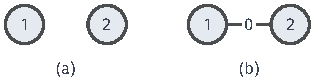
\includegraphics[width=53.188mm]{figures/01-basic-mathematics/04-graphs/tikz/c1-zero-weight-edge/figure.pdf}
  \caption{无边(a)与零权边(b)。二者在数值上都记为$0$，但只有(b)中顶点$1,2$相邻。}
  \label{fig:graph-conn-zero-weight}
\end{figure}

\paragraph{顶点属性与边属性}
边上还可以记录类别、时间等数据，顶点上也可以记录人口、坐标等数据，分别称为边属性和顶点属性。顶点的名称$1,2,3,4$只用来区分顶点，本身不是属性。第~\ref{sec:graph-isomorphism}节会看到，换一套名称不改变图的结构，而属性是否也必须保持，要由问题来规定。

\subsection{子图与诱导子图}
\label{sec:graph-conn-subgraphs}

研究道路网时，我们常常只关心其中一部分城市，或者想知道封闭几条道路以后还剩下什么。取出的部分要仍是一张图，只需保证留下的每条边两个端点都还在。正式地说，若$V'\subseteq V$，$E'\subseteq E$，并且$E'$中每条边的两个端点都在$V'$中，称$\mathcal G'=(V',E')$是$\mathcal G$的\term{子图}（subgraph）。

最常用的两种子图来自删除操作。删除一条边$e$只去掉这条边，记作$\mathcal G-e$；删除一个顶点集$S$则去掉$S$中的顶点，连同所有至少有一个端点在$S$中的边，记作$\mathcal G-S$。删除顶点时必须连带删边，否则留下的边会缺少端点，不再构成子图。

图~\ref{fig:graph-conn-subgraph-induced}(d)只删除了边$\{2,3\}$。(b)(c)保留了同一组顶点$\{1,2,3\}$，边集却不同，可见只给出顶点集合还不能确定一个子图。

\begin{figure*}[!htb]
  \centering
  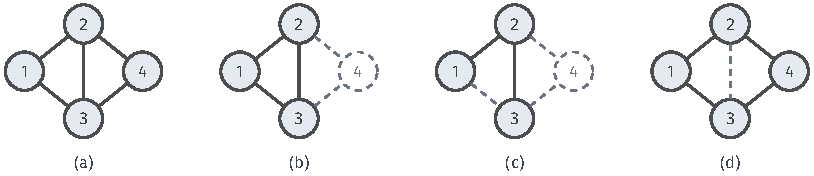
\includegraphics[width=137.686mm]{figures/01-basic-mathematics/04-graphs/tikz/c1-subgraph-induced/figure.pdf}
  \caption{贯穿图的几种子图，灰色虚线表示被删除的顶点或边。(b)删除顶点$4$及其两条边，恰好得到顶点集$\{1,2,3\}$上的诱导子图；(c)保留同样三个顶点，却漏掉了原图中的边$\{1,3\}$，是子图但不是诱导子图；(d)只删除一条边，顶点全部保留。}
  \label{fig:graph-conn-subgraph-induced}
\end{figure*}

\paragraph{诱导子图}
只研究一部分顶点时，通常不希望悄悄改变这些顶点之间的关系，于是把原图中两端都在其中的边全部保留下来。

\begin{definition}[诱导子图]
\label{def:graph-conn-induced-subgraph}
设$S\subseteq V$。以$S$为顶点集、以$\{\{i,j\}\in E:i,j\in S\}$为边集的子图，称为$\mathcal G$在$S$上的\term{诱导子图}（induced subgraph），记作$\mathcal G[S]$。有向图的诱导子图保留两端都在$S$中的全部弧。
\end{definition}

与一般子图不同，诱导子图由顶点集唯一确定。构造$\mathcal G[S]$时，标记$S$中的顶点，再逐条扫描边，两端都有标记的就保留。

对贯穿图取$S=\{1,2,3\}$，保留$\{1,2\},\{1,3\},\{2,3\}$，舍去含$4$的两条边，得到图~\ref{fig:graph-conn-subgraph-induced}(b)。核对一个声称的诱导子图，还要反过来检查原图中两端都在$S$中的边是否一条不漏；图(c)漏掉了$\{1,3\}$，所以不是诱导子图。

删除顶点得到的也是诱导子图。$\mathcal G-S$删去的恰好是至少一端在$S$中的边，留下的恰好是两端都在$V\setminus S$中的边，所以$\mathcal G-S=\mathcal G[V\setminus S]$；例如图(b)既是$\mathcal G[\{1,2,3\}]$，也是$\mathcal G-\{4\}$。第~\ref{sec:graph-connectivity-separation}节讨论删除顶点能否切断连接，第~\ref{chap:graph-traversal}章按分隔集把图分块，用到的都是这两种写法。

\section{邻接与路径}
\label{sec:graph-adjacency-paths}

贯穿图\eqref{eq:graph-conn-running-graph}中顶点$1$和$4$之间没有边，却可以先到$2$或$3$，再到$4$。一步能到谁，由边集直接读出；若干步能到谁，要把边首尾相接。本节从一个顶点的直接邻居出发，把一步的连接延长为行走和路径，由此得到环与可达关系。比较不同路线的总长度是第~\ref{chap:shortest-paths}章的问题，这里只讨论哪些顶点序列允许通行。

\subsection{邻接、邻域与度}
\label{sec:graph-conn-neighborhoods}

站在一座城市，首先要知道哪些城市与它有直达道路，这样的城市有几座。在无向图中，若$\{i,j\}\in E$，称$i$与$j$\term{邻接}（adjacent），互为邻居。顶点$i$的全部邻居组成它的\term{邻域}（neighborhood）
\[
N(i)=\{j\in V:\{i,j\}\in E\},
\]
邻居的个数$d_i=|N(i)|$称为$i$的\term{度}（degree）。

贯穿图中$N(1)=\{2,3\}$，$N(2)=\{1,3,4\}$，四个顶点的度依次为$2,3,3,2$。度只数直接邻居，经两步才能到达的$4$不计入$N(1)$。

在有向的依赖关系中，还要分清“我直接依赖谁”和“谁直接依赖我”：弧$i\to j$对两端的意义不同。因此分别定义出邻域与入邻域
\[
N^+(i)=\{j:(i,j)\in E\},\qquad
N^-(i)=\{j:(j,i)\in E\},
\]
二者的大小$d_i^+$与$d_i^-$分别称为\term{出度}（out-degree）与\term{入度}（in-degree）。图~\ref{fig:graph-conn-neighborhood-degree}在贯穿图和一个小有向图上标出了这些量。

\begin{figure}[!htb]
  \centering
  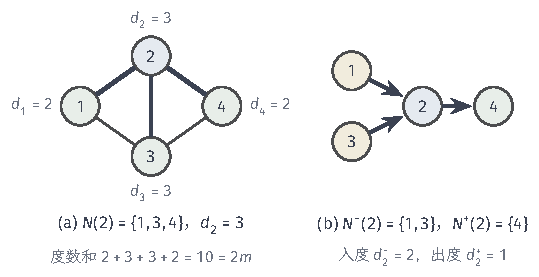
\includegraphics[width=91.271mm]{figures/01-basic-mathematics/04-graphs/tikz/c1-neighborhood-degree/figure.pdf}
  \caption{邻域与度。(a)贯穿图中顶点$2$的邻域$N(2)=\{1,3,4\}$（绿色），连接它们的三条边加粗，所以$d_2=3$；顶点旁标出各点的度，四个度之和$10$恰为边数的两倍。(b)有向图$1\to2$、$3\to2$、$2\to4$中，顶点$2$的入邻域$N^-(2)=\{1,3\}$（黄色）与出邻域$N^+(2)=\{4\}$（绿色），入度为$2$，出度为$1$。}
  \label{fig:graph-conn-neighborhood-degree}
\end{figure}

\paragraph{度数和与边数}
考虑所有“顶点—边”配对$(i,e)$，其中$i$是边$e$的端点。按顶点分组，顶点$i$出现在$d_i$个配对中；按边分组，每条边恰有两个端点。两种分组数的是同一批配对，所以
\begin{equation}
\sum_{i\in V}d_i=2m.
\label{eq:graph-conn-handshake}
\end{equation}
由此可知度为奇数的顶点个数必是偶数。有向图中每条弧恰好贡献一个出度和一个入度，所以$\sum_i d_i^+=\sum_i d_i^-=m$。

\paragraph{邻域与度的读取}
给每个顶点准备一个空的邻居集合和一个初始为$0$的计数器，然后逐条读边：读到$\{i,j\}$时，把$j$放进$N(i)$、$i$放进$N(j)$，两个计数器各加$1$。表~\ref{tab:graph-conn-degree-trace}是贯穿图上计数器的变化。每读一条边，度数和加$2$，读完$m$条边就是$2m$，这正是式\eqref{eq:graph-conn-handshake}；最后一列若不等于两倍边数，说明某条边只记了一端。

有向图读到弧$(i,j)$时，把$j$放进$N^+(i)$、$i$放进$N^-(j)$。图~\ref{fig:graph-conn-direction-orientation}(c)的$1\to2\leftarrow3$读完后$N^-(2)=\{1,3\}$，$N^+(2)=\varnothing$；不说明方向，就可能把入邻居误当成下一步可以到达的顶点。这里的度只数结构上的边；边带权时把一个顶点所有邻边的权相加，得到的是另一个量，本部分不使用。

\begin{table}[!htb]
  \centering
  \caption{逐条读入贯穿图的边时，四个度计数器的变化。每读一条边，恰有两个计数器各加$1$，度数和每次增加$2$。}
  \label{tab:graph-conn-degree-trace}
  \small
  \begin{tabular}{@{}lccccc@{}}
    \toprule
    已读入的边 & $d_1$ & $d_2$ & $d_3$ & $d_4$ & 度数和\\
    \midrule
    初始 & $0$ & $0$ & $0$ & $0$ & $0$\\
    $\{1,2\}$ & $1$ & $1$ & $0$ & $0$ & $2$\\
    $\{1,3\}$ & $2$ & $1$ & $1$ & $0$ & $4$\\
    $\{2,3\}$ & $2$ & $2$ & $2$ & $0$ & $6$\\
    $\{2,4\}$ & $2$ & $3$ & $2$ & $1$ & $8$\\
    $\{3,4\}$ & $2$ & $3$ & $3$ & $2$ & $10$\\
    \bottomrule
  \end{tabular}
\end{table}

\subsection{行走、路径与环}
\label{sec:graph-conn-walks-paths}

走一步就是从当前顶点走到它的一个邻居，走若干步就得到一串相邻两项都邻接的顶点。是否允许重复经过顶点要看用途：计数多步走法时允许重复，一条实际路线通常不允许。

\begin{definition}[行走与路径]
\label{def:graph-conn-walk-path}
设$\mathcal G=(V,E)$是无向图。顶点序列$(v_0,\ldots,v_k)$若对每个$r=1,\ldots,k$都有$\{v_{r-1},v_r\}\in E$，就称为从$v_0$到$v_k$的一条\term{行走}（walk），$k$称为它的长度，即经过的边数。若行走中的顶点两两不同，就称为一条简单\term{路径}（path）。
\end{definition}

单个顶点$(v_0)$是长度为零的行走，也是长度为零的路径。本部分不加修饰的“路径”都指简单路径。

绕一圈回到起点的路线还要与原路折返区分开。首尾相同（$v_0=v_k$）的行走称为\term{闭行走}（closed walk），但闭合不意味着绕成一圈：沿一条边去而复返的$(2,4,2)$是闭行走，却没有提供第二条路线。

因此把长度$k\geq3$、且$v_0,\ldots,v_{k-1}$两两不同的闭行走称为\term{环}（cycle）；长度为$1$的闭行走需要自环，长度为$2$的只能沿同一条边往返，所以要求$k\geq3$。同一个环可以从不同顶点出发、沿两个方向书写，例如$(1,2,3,1)$与$(1,3,2,1)$，我们把经过同一组边的序列看成同一个环。

\paragraph{顶点序列的核对}
判断一个顶点序列属于哪一类，按定义依次检查：每一步$\{v_{r-1},v_r\}$是否为边，判断行走；从左到右维护“已出现顶点”的集合，看有无重复，判断路径；再要求$k\geq3$、首尾相同且前$k$个顶点不重复，判断环。

图~\ref{fig:graph-conn-walk-path-cycle}给出四个结果：$(1,2,3,1,2)$是行走，但第二次读到$1$时重复，不是路径；$(1,2,4)$是路径；$(2,4,2)$是闭行走而不是环；$(1,2,3,1)$是环。

三者逐步加强，反过来都不成立：行走便于拼接与计数，路径对应实际路线，环表示存在替代路线。

\begin{figure*}[!htb]
  \centering
  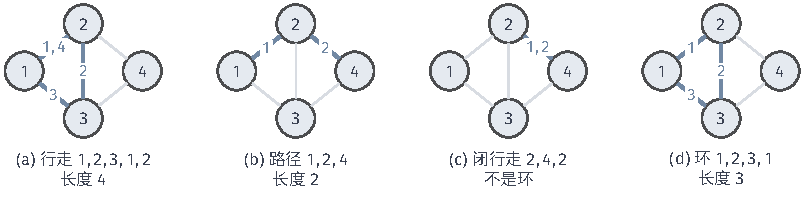
\includegraphics[width=136.186mm]{figures/01-basic-mathematics/04-graphs/tikz/c1-walk-path-cycle/figure.pdf}
  \caption{贯穿图上的四种顶点序列。蓝色粗线是经过的边，边旁数字是经过该边的步序，浅灰色是未经过的边。(a)行走可以重复经过边$\{1,2\}$；(b)路径不重复顶点；(c)沿一条边去而复返得到闭行走，但它不是环；(d)绕三角形一周的环除首尾外不重复顶点。}
  \label{fig:graph-conn-walk-path-cycle}
\end{figure*}

\subsection{有向路径与有向无环图}
\label{sec:graph-conn-dag}

任务依赖要求每一步都顺着箭头走。若顺着箭头走一圈又回到出发的任务，例如$1$等$2$、$2$等$3$、$3$又等$1$，这组任务就无法按任何次序全部完成。把定义~\ref{def:graph-conn-walk-path}中的条件换成$(v_{r-1},v_r)\in E$，就得到有向行走与\term{有向路径}（directed path）。除首尾外顶点两两不同、长度至少为$1$的有向闭行走称为\term{有向环}（directed cycle）；由于没有自环，其长度至少为$2$。

\begin{definition}[有向无环图]
\label{def:graph-conn-dag}
不含有向环的有向图称为\term{有向无环图}（directed acyclic graph，DAG）。
\end{definition}

有向环的最短长度与无向情形不同。图~\ref{fig:graph-conn-directed-cycle-dag}(a)中两条反向弧$i\to j$和$j\to i$是两个不同的对象，$(i,j,i)$构成长度为$2$的有向环；无向图中的$(2,4,2)$两次经过的是同一条边。图(b)的$(1,2,3,1)$每一步都顺着箭头，是长度为$3$的有向环。

\begin{figure}[!htb]
  \centering
  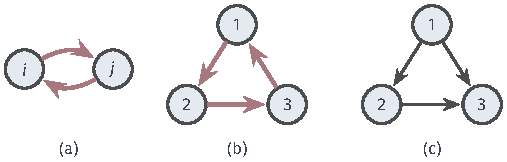
\includegraphics[width=85.937mm]{figures/01-basic-mathematics/04-graphs/tikz/c1-directed-cycle-dag/figure.pdf}
  \caption{有向环与有向无环图。红色弧组成有向环。(a)两条反向弧构成长度为$2$的有向环；(b)三角形的循环定向含有向环；(c)同一个三角形的另一种定向不含有向环，是有向无环图，尽管它的底层无向图是一个环。}
  \label{fig:graph-conn-directed-cycle-dag}
\end{figure}

\paragraph{无环的核对}
有向环上的每个顶点都有环上的弧进出，所以入度或出度为$0$的顶点不在任何有向环上。图~\ref{fig:graph-conn-directed-cycle-dag}(c)的弧为$1\to2$、$1\to3$、$2\to3$，$1$的入度与$3$的出度为$0$，剩下的顶点$2$不足以构成至少含两个顶点的有向环，所以它是DAG。大图上系统地判断有无有向环，要用第~\ref{sec:graph-dfs}节的深度优先遍历或第~\ref{sec:graph-topological-order}节的拓扑排序。

图(c)是DAG，它的底层无向图却是三角形。拓扑排序要求的正是有向无环；换成“底层无向图无环”这一更强的条件，会把(c)这样完全可以排出次序的依赖错误地排除。

\subsection{可达性}
\label{sec:graph-conn-reachability}

很多问题只关心从$i$出发能不能到达$j$，而不关心怎么到。若存在从$i$到$j$的行走，称$j$从$i$\term{可达}（reachable）；有向图中要求有向行走。行走首尾相接仍是行走，路径则未必，所以用行走定义更方便。下面的引理说明改用路径定义并无区别。

\begin{lemma}[行走中含有路径]
\label{lem:graph-conn-walk-contains-path}
在无向图或有向图中，若存在从$i$到$j$的行走，则存在从$i$到$j$的路径，并且它的顶点和边都取自这条行走。
\end{lemma}

\begin{proof}
在从$i$到$j$、顶点和边都取自原行走的所有行走中，取长度最短的一条$(v_0,\ldots,v_k)$。若它不是路径，则有$s<t$使$v_s=v_t$。删去中间段$v_{s+1},\ldots,v_t$，得到$(v_0,\ldots,v_s,v_{t+1},\ldots,v_k)$：原来从$v_t$出发的那一步现在从$v_s=v_t$出发，每一步仍沿原有的边或弧，而长度减少了$t-s>0$，矛盾。
\end{proof}

\paragraph{从行走中取出路径}
实际取出路径时，可以从左到右读一遍行走，随读随删。维护当前路径$P$，初始为$(v_0)$，并给$P$上的顶点做标记。读到$v_r$时，若它没有标记，就接到$P$末尾；若已有标记，说明$P$绕回了$v_r$，就把$P$截到$v_r$所在的位置，并清除其后的标记。$P$始终顶点互异、各边取自原行走，读完时就是所求的路径。每个顶点至多接上、删去各一次，工作量与行走长度成正比。

以行走$(1,2,3,1,3,4)$为例，$P$依次为$(1)$、$(1,2)$、$(1,2,3)$，读到第二个$1$时截回$(1)$，再变为$(1,3)$、$(1,3,4)$。

\paragraph{可达关系的性质}
零长度行走给出自反性，行走首尾相接给出传递性；无向图中把行走倒过来走仍是行走，所以还有对称性。同时满足自反、对称、传递三条的二元关系称为等价关系，所以无向图上的可达关系是等价关系。等价关系的等价类两两不交、并起来恰为全集，下一节据此划分连通分量；等价关系与划分的一般对应，可参考\BookChapterRef{chap:sets-relations-maps}{卷一第~\ref{chap:sets-relations-maps}章}。

这里的性质只说明可达关系是什么。给出两个具体顶点、要判断是否可达，仍需要有组织地访问能走到的顶点，这是第~\ref{sec:graph-bfs}节与第~\ref{sec:graph-dfs}节的任务。

有向图中倒过来走需要反向弧，对称性不再成立：单向链$1\to2\to3$中，$3$从$1$可达，$1$却不从$3$可达。为描述这种单向关系，$N^-(j)$中的顶点称为$j$的直接\term{前驱}（predecessor），$N^+(j)$中的顶点称为直接\term{后继}（successor）；能经一条或多条弧到达$j$的其他顶点称为$j$的\term{祖先}（ancestor），从$j$出发经一条或多条弧能到达的其他顶点称为$j$的\term{后代}（descendant）。本部分约定祖先与后代都不含$j$自身。

单向链中$3$的直接前驱只有$2$，祖先是$\{1,2\}$；$1$的后代是$\{2,3\}$。

有向环上的两个不同顶点可以互为祖先，在DAG中这不可能发生：若$i\neq j$互为祖先，两条有向路径拼成长度至少为$2$的有向闭行走$(v_0,\ldots,v_k)$；在所有满足$s<t$、$v_s=v_t$的位置对中取$t-s$最小的一对，$(v_s,\ldots,v_t)$除首尾外不重复顶点，长度又不能为$1$，所以是有向环，矛盾。可达的不对称使有向图的“连通”需要两种定义，这是下一节的内容。

\section{连通与分隔}
\label{sec:graph-connectivity-separation}

上一节的可达关系一次只回答两个顶点之间的问题。道路网规划还需要整体的回答：全部城市分成几片互相到达的区域，封闭哪些路口或道路会把区域切开。前一个问题由可达关系的等价类回答，有向图中则要区分强、弱两种连通；后一个问题要看删除顶点或边以后是否还有替代路径。这里只讨论结构上的路径是否存在；概率模型中的条件独立另有自己的分离判据，不在本卷讨论。

\subsection{无向图的连通分量}
\label{sec:graph-conn-components}

我们想把全部城市分成若干片，同一片中的城市两两可以互相到达，不同片之间无路可通；有了这样的划分，“能否互相到达”就只需看是否在同一片中。第~\ref{sec:graph-conn-reachability}小节说明，无向图中的可达关系是等价关系；等价类两两不交、并起来恰为$V$，所以它们恰好构成这样的划分。

\begin{definition}[连通分量]
\label{def:graph-conn-component}
无向图$\mathcal G=(V,E)$中可达关系的每个等价类$C\subseteq V$称为$\mathcal G$的一个\term{连通分量}（connected component）；有时也把诱导子图$\mathcal G[C]$称为连通分量。若$\mathcal G$非空且恰有一个连通分量，即任意两个顶点之间都有路径，就称$\mathcal G$是\term{连通}（connected）的。
\end{definition}

这个划分有三条直接的性质。连接同一分量中两点的路径不会离开该分量，因为路径上的每个顶点都与起点可达，所以$\mathcal G[C]$本身连通。不同分量之间没有边，否则两端可达，应属同一分量。划分只取决于可达关系，由图唯一确定。

图~\ref{fig:graph-conn-components}(a)是三角形$\{1,2,3\}$加上孤立顶点$4$，有两个分量$\{1,2,3\}$与$\{4\}$，不连通。空图的分量数为$0$，按定义不算连通，用“恰有一个分量”判断连通时要先排除这个情形。

\begin{figure*}[!htb]
  \centering
  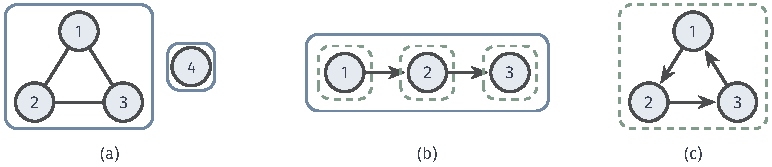
\includegraphics[width=130.652mm]{figures/01-basic-mathematics/04-graphs/tikz/c1-components/figure.pdf}
  \caption{连通分量。蓝色实线框是无向图或底层无向图的连通分量，绿色虚线框是强连通分量。(a)孤立点自成一个分量；(b)单向链$1\to2\to3$忽略方向后连成一片，但没有两个顶点能互相到达，每个顶点自成一个强分量；(c)有向环上任意两个顶点都能互相到达，三个顶点属于同一个强分量。}
  \label{fig:graph-conn-components}
\end{figure*}

\paragraph{分量划分的核对}
核对别人给出的划分不必逐对找路径，上面的前两条性质反过来就够了。

\begin{lemma}[分量划分的核对]
\label{lem:graph-conn-component-check}
设$C_1,\ldots,C_c$是无向图$\mathcal G$的顶点集的一个划分。若每个$\mathcal G[C_k]$都连通，并且没有一条边的两端位于不同的块中，则$C_1,\ldots,C_c$恰好是$\mathcal G$的全部连通分量。
\end{lemma}

\begin{proof}
同一块中的两点由块内连通而可达。反过来，若$j$从$i$可达，取一条行走，它的每一步沿一条边，而没有边跨越不同的块，所以$i,j$在同一块中。于是各块就是可达关系的等价类。
\end{proof}

于是核对分两步：给顶点写上块编号，逐条扫描边，检查两端编号相同；再对每一块给出把块内顶点连在一起的边。图~\ref{fig:graph-conn-components}(a)的划分$(1,1,1,2)$两步都通过；若把贯穿图划分为$\{1,2\}$与$\{3,4\}$，第一步就在边$\{1,3\}$处失败。

第二步所需的块内连接在第~\ref{sec:graph-trees-forests}节整理为生成森林；从零求出全部分量，由第~\ref{sec:graph-connectivity-computation}节在与$n+m$成正比的时间内完成。

一张图是否连通，取决于删去连接以后有没有替代路径。在贯穿图中删除边$\{2,3\}$，$2$与$3$仍可经$1$或$4$相连；在图~\ref{fig:graph-conn-cut-bridge}(a)中删除连接两个三角形的边$\{3,4\}$，图就分成两个分量。两次都只删除一条边，结果不同是因为前者的边位于环上，环的另一侧提供了替代路径。第~\ref{sec:graph-conn-cut-bridge}小节会把这一观察写成桥的判别条件。

\subsection{强连通与弱连通}
\label{sec:graph-conn-strong-weak}

有向图中可达不是等价关系，不能直接用来划分顶点。修补的办法有两种：要求双向都可达，回答哪些顶点能“绕得回来”；或者忽略方向，只问是否连成一片。

若$j$从$i$可达且$i$从$j$可达，称$i,j$相互可达。相互可达关系是自反的（零长度行走）、对称的（定义对$i,j$对称）、传递的（两个方向分别首尾相接），因此是等价关系。它的等价类称为\term{强连通分量}（strongly connected component）；若有向图非空且只有一个强连通分量，就称它\term{强连通}（strongly connected）。

忽略方向的办法用底层无向图（第~\ref{sec:graph-conn-directions}小节）的连通分量划分顶点，所得的分量称为原图的\term{弱连通分量}（weakly connected component）；底层无向图连通时，称原有向图\term{弱连通}（weakly connected）。

在小图上可以直接读出两种分量。记$R^+(v)$与$R^-(v)$分别为从$v$可达与能到达$v$的顶点集（都含$v$），由定义，$v$所在的强分量是
\[
R^+(v)\cap R^-(v);
\]
弱分量则在底层无向图上读出。

图~\ref{fig:graph-conn-components}(b)的单向链中，$R^+(2)=\{2,3\}$，$R^-(2)=\{1,2\}$，所以$2$所在的强分量是
\[
R^+(2)\cap R^-(2)=\{2,3\}\cap\{1,2\}=\{2\}.
\]
同理三个顶点各成一个强分量，却只有一个弱分量。(c)的有向环中两个可达集都是$\{1,2,3\}$，图强连通。在大图上求全部强分量的线性时间方法见第~\ref{sec:graph-connectivity-computation}节。

有向路径去掉箭头后是底层无向图中的路径，所以每个强分量都包含在某个弱分量之内，强连通蕴含弱连通。单向链说明反过来不成立。需要回答“能否往返”时，必须使用强分量。

\subsection{分隔集}
\label{sec:graph-conn-separators}

规划者还关心脆弱性：封闭哪些路口能把两个区域隔开。被封闭的路口不能属于要隔开的两组本身；“隔开”的含义是，删掉这些路口以后，两组之间一条路径也不剩。

\begin{definition}[分隔]
\label{def:graph-conn-separation}
设$A,B,S\subseteq V$两两不相交。若在$\mathcal G-S$中不存在从$A$中顶点到$B$中顶点的路径，就称$S$\term{分隔}（separate）$A$与$B$，称$S$为$A$与$B$之间的一个\term{分隔集}（separator）。
\end{definition}

等价地，$\mathcal G$中从$A$到$B$的每条路径都至少经过$S$中的一个顶点，因为$\mathcal G-S$中的路径就是$\mathcal G$中避开$S$的路径。所以验证一个候选集要考虑全部路径，找到一条被阻断的路径并不够。

核对时却不必列举路径：在$\mathcal G-S$中从$A$出发求出可达集$R$（第~\ref{sec:graph-bfs}节的广度优先遍历允许以一组顶点为起点），$S$分隔$A$与$B$当且仅当$R\cap B=\varnothing$。若$A$与$B$原本位于不同分量，空集就分隔它们。

在图~\ref{fig:graph-conn-separator-sets}中取$A=\{1\}$、$B=\{4\}$。删除$\{2\}$后$R=\{1,3,4\}$，路径$(1,3,4)$仍在，$\{2\}$不是分隔集；删除$\{2,3\}$后$1$的邻居全被删去，$R=\{1\}$，$\{2,3\}$是分隔集。

\begin{figure}[!htb]
  \centering
  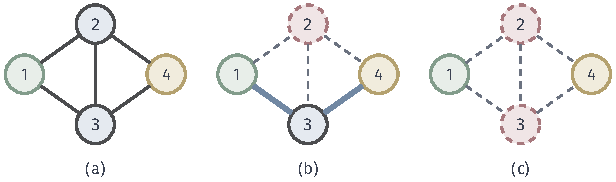
\includegraphics[width=104.186mm]{figures/01-basic-mathematics/04-graphs/tikz/c1-separator-sets/figure.pdf}
  \caption{在贯穿图中检验分隔集，$A=\{1\}$为绿色，$B=\{4\}$为黄色，被删除的候选集$S$为红色虚线顶点。(b)删除$\{2\}$后蓝色路径$(1,3,4)$仍然存在，$\{2\}$不是分隔集；(c)删除$\{2,3\}$后从$1$到$4$没有路径，$\{2,3\}$分隔$\{1\}$与$\{4\}$。}
  \label{fig:graph-conn-separator-sets}
\end{figure}

不指定两组顶点时，分隔集由删除后的分量给出。对连通图$\mathcal G$，若$\mathcal G-S$不连通，则$S$分隔$\mathcal G-S$中任意两个不同分量的顶点集。例如贯穿图删除$\{2,3\}$后余下$\{1\}$与$\{4\}$。第~\ref{sec:graph-separator-blocks}节将沿这样的分隔集把图分成可以分别处理的块。

\subsection{割点与桥}
\label{sec:graph-conn-cut-bridge}

最脆弱的情形是只失去一个路口或一条道路，网络就断开。删除顶点$v$后$\mathcal G-\{v\}$的分量数大于$\mathcal G$的分量数，称$v$为\term{割点}（cut vertex）；删除边$e$后$\mathcal G-e$的分量数大于$\mathcal G$的分量数，称$e$为\term{桥}（bridge）。

图~\ref{fig:graph-conn-cut-bridge}(a)由两个三角形$\{1,2,3\}$、$\{4,5,6\}$和边$\{3,4\}$组成，$3,4$是割点，$\{3,4\}$是桥，三角形内部的边和顶点$1,2,5,6$都不是；(b)的链中，中间顶点$2$是割点，两条边都是桥；(c)的三角形中，删除任意一个顶点或一条边都不会断开。

\begin{figure*}[!htb]
  \centering
  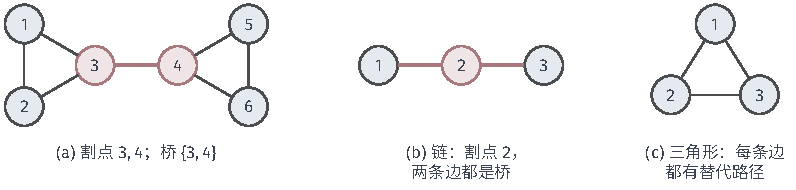
\includegraphics[width=132.687mm]{figures/01-basic-mathematics/04-graphs/tikz/c1-cut-vertex-bridge/figure.pdf}
  \caption{割点与桥，红色顶点为割点，红色粗边为桥。(a)两个三角形由一条边相连，这条边是桥，它的两个端点是割点；(b)链上每条边都是桥，中间顶点是割点，端点$1,3$虽是桥的端点却不是割点；(c)三角形的每条边都位于环上，删除任何一条边或一个顶点都不会断开。}
  \label{fig:graph-conn-cut-bridge}
\end{figure*}

\paragraph{桥的判别}
按定义判断桥要比较删除前后的分量数。下面的定理把它换成只看这条边两端的条件，并说明环正是替代路径的来源。

\begin{theorem}[桥的判别]
\label{thm:graph-conn-bridge-cycle}
设$e=\{i,j\}$是无向图$\mathcal G$的一条边。以下三条等价：(1)$e$是桥；(2)$\mathcal G-e$中没有从$i$到$j$的路径；(3)$e$不在$\mathcal G$的任何环上。并且删除任何一条边，分量数至多增加$1$。
\end{theorem}

\begin{proof}
删除$e$只可能拆开$e$所在的分量$C$。$C$中任一顶点$x$在原图中有到$i$的路径；若它经过$e$，取它第一次到达$i$或$j$之前的部分。这部分不含$e$，所以删除后$x$仍连到$i$或$j$。因此$\mathcal G-e$中$C$至多分成$i$所在和$j$所在两部分，分量数至多增加$1$，并且增加当且仅当$i,j$不再连通，即(1)与(2)等价。

若$e$在某个环上，环的另一侧就是$\mathcal G-e$中从$i$到$j$的路径，所以(2)蕴含(3)；反过来，$\mathcal G-e$中从$i$到$j$的路径长度至少为$2$，接上$e$就是一个环，所以(3)蕴含(2)。
\end{proof}

\paragraph{割点与桥的检验}
由定理，检验$e=\{i,j\}$是否为桥，只需在$\mathcal G-e$中从$i$做一次可达性搜索，看能否到达$j$。例如在图~\ref{fig:graph-conn-cut-bridge}(a)中，删去$\{3,4\}$后从$3$只能到达$\{1,2,3\}$，它是桥；删去$\{1,2\}$后仍可经$3$到达$2$，它不是桥。

检验顶点$v$是否为割点，则删去$v$后从它的一个邻居出发，看能否到达它的其余全部邻居。只看邻居就够了：$v$所在分量中的其他顶点，沿通往$v$的路径走到第一次遇到$v$的邻居为止，这一段避开了$v$，所以它们在删去$v$后仍连到$v$的某个邻居。于是分量是否断开，只取决于$v$的邻居之间是否仍然连通。逐一检验全部顶点或全部边，每次都要做一次这样的搜索。

删点与删边的效果并不对称。删除一个顶点会同时删除它的全部邻边，可能把分量拆成很多块：星形图删除中心顶点后，其余每个顶点都自成一个分量；删除一条边却至多增加一个分量。桥的端点不一定是割点，例如图~\ref{fig:graph-conn-cut-bridge}(b)的端点$1$；没有桥的图也可能有割点，例如两个三角形共用一个顶点。所以“删点能否断开”与“删边能否断开”需要分别检查。

\section{树与森林}
\label{sec:graph-trees-forests}

上一节看到，边位于环上时删掉它不会断开连接，环提供的是冗余的替代路径。若要用尽量少的道路把一组城市连起来，就不应保留任何环。本节研究这种连通而无环的结构。树的两个条件分别对应路径的存在与唯一，由此能数出树的边数，边数又反过来给出判断树的简便方法。

此后两小节讨论树的两种用法：在树上选根可以组织上下层次，在一般连通图中则可以抽出一棵覆盖全部顶点的树。这些结论是第~\ref{chap:graph-traversal}章遍历结果、第~\ref{sec:graph-minimum-spanning-tree}章最小生成树和第~\ref{sec:graph-tree-dp}节树上动态规划的共同基础。

\subsection{树与森林的定义}
\label{sec:graph-conn-tree-definition}

不修多余道路的道路网应当连通，以保证任意两点之间都有路线；还应当无环，因为由定理~\ref{thm:graph-conn-bridge-cycle}，环上的边删去后图仍然连通，可以省掉。同时要求这两点就得到树，只要求无环得到的是若干互不相连的树。

\begin{definition}[树与森林]
\label{def:graph-conn-tree}
非空、连通且不含环的无向图称为\term{树}（tree）。不含环的无向图称为\term{森林}（forest）。
\end{definition}

森林的每个连通分量都连通且无环，是一棵树；只有恰好一个分量的森林才是树。

图~\ref{fig:graph-conn-tree-forest}中，(a)的链和(b)的星形都是树，树可以有分支；(c)的三角形连通但有环，不是树；(d)有三个分量，每个都是树，整体是森林。

两个边界情形需要注意。只有一个顶点、没有边的图是单点树，所以树中的顶点不必都有邻边。空图不含环，是有$0$个分量的空森林，但树要求非空，所以空图不是树。

\begin{figure*}[!htb]
  \centering
  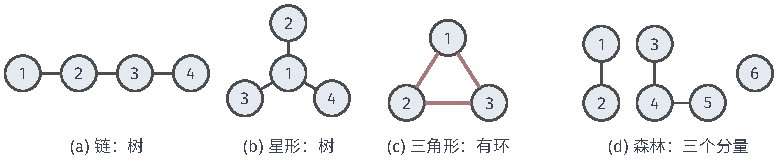
\includegraphics[scale=1]{figures/01-basic-mathematics/04-graphs/tikz/c1-tree-forest/figure.pdf}
  \caption{树、森林与非树的对照。(a)链与(b)星形都是树，后者有分支；(c)三角形连通但含有红色标出的环，不是树；(d)由三个互不相连的树组成的森林，其中孤立顶点$6$是一棵单点树。}
  \label{fig:graph-conn-tree-forest}
\end{figure*}

\subsection{树的基本性质}
\label{sec:graph-conn-tree-properties}

\paragraph{路径唯一性}
树的连通保证任意两点之间有路径，无环则保证这样的路径只有一条。直观上，若两点之间有两条不同的路径，它们分开以后终究要会合，分开与会合之间的两段就围成一个环；反过来，环上相邻的两点既有一条边直接相连，又可以沿环的另一侧到达。

\begin{theorem}[树中路径唯一]
\label{thm:graph-conn-tree-unique-path}
设$\mathcal G$是非空无向图。$\mathcal G$是树，当且仅当任意两个顶点之间恰有一条路径。
\end{theorem}

\begin{proof}
先设$\mathcal G$是树。连通性保证任意两点$u,v$之间至少有一条路径。假设有两条不同的路径$P=(p_0,\ldots,p_a)$与$Q=(q_0,\ldots,q_b)$，$p_0=q_0=u$，$p_a=q_b=v$。一条不能是另一条的真前段，否则较长的那条会两次经过$v$；所以存在最小的$s$使$p_{s+1}\neq q_{s+1}$，记$x=p_s=q_s$。由于$v$同时在两条路径上，可以取$P$在$x$之后第一个也出现在$Q$中$x$之后的顶点$y$。

$P$从$x$到$y$的一段与$Q$从$x$到$y$的一段除端点外没有公共顶点：$P$这一段的中间顶点按$y$的取法不在$Q$中$x$之后的部分，又因为$P$是路径，也不在两者共有的$x$之前的部分。沿$P$从$x$走到$y$，再沿$Q$倒着走回$x$，得到一个除首尾外不重复顶点的闭行走。两段不能都只有一条边，否则$p_{s+1}=y=q_{s+1}$；所以它的长度至少为$3$，是一个环，矛盾。图~\ref{fig:graph-conn-tree-properties}画出了这个构造。

反过来，设任意两点之间恰有一条路径，则$\mathcal G$连通。若$\mathcal G$含环$(c_0,c_1,\ldots,c_{k-1},c_0)$，$k\geq3$，则$(c_0,c_1)$与$(c_0,c_{k-1},\ldots,c_1)$是从$c_0$到$c_1$的两条不同路径，矛盾。
\end{proof}
\begin{BookInlineFigure}
  \centering
  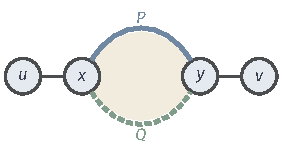
\includegraphics[scale=1]{figures/01-basic-mathematics/04-graphs/tikz/c1-tree-properties/figure.pdf}
  \caption{两条不同路径会围出环。路径$P$（蓝色实线）与$Q$（绿色虚线）在$x$分开、在$y$第一次会合；它们之间的两段构成黄色区域的边界，因此树中不可能同时存在这两条路径。}
  \label{fig:graph-conn-tree-properties}
\end{BookInlineFigure}

由这个定理，删除树的任意一条边$e=\{u,v\}$后$u,v$之间不再有路径，由定理~\ref{thm:graph-conn-bridge-cycle}，树恰好分成两棵较小的树。树的每条边都是桥。

\paragraph{边数}
数树的边数要用到度为$1$的顶点，称为\term{叶}（leaf）。叶只与一个顶点相连，删掉它不会断开其余部分，这使我们能对顶点数归纳。先说明叶总是存在。

\begin{lemma}[树有叶]
\label{lem:graph-conn-tree-leaves}
至少有两个顶点的树至少有两个叶。
\end{lemma}

\begin{proof}
取一条最长的路径$P=(v_0,\ldots,v_k)$，由于树连通且至少有两个顶点，$k\geq1$。若$v_0$另有邻居$z\neq v_1$：$z$不在$P$上时，$(z,v_0,\ldots,v_k)$是更长的路径；$z=v_t$在$P$上时$t\geq2$，$(v_0,v_1,\ldots,v_t,v_0)$是环。两种情形都不可能（图~\ref{fig:graph-conn-tree-properties-leaf}），所以$d_{v_0}=1$。同理$d_{v_k}=1$。
\end{proof}
\begin{BookInlineFigure}
  \centering
  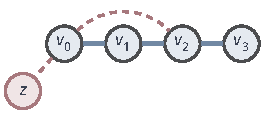
\includegraphics[scale=1]{figures/03-graphs/01-structure-and-computation/tikz/tree-longest-path-leaf/figure.pdf}
  \caption{最长路径的端点必须是叶。若端点$v_0$另有邻居，邻居在路径外（如$z$）会使路径延长，在路径上（如$v_2$）则会形成环；红色虚线表示这两种不可能的连接。}
  \label{fig:graph-conn-tree-properties-leaf}
\end{BookInlineFigure}

\begin{theorem}[树的边数]
\label{thm:graph-conn-tree-edges}
有$n$个顶点的树恰有$n-1$条边。
\end{theorem}

\begin{proof}
对$n$归纳，$n=1$时单点树没有边。设$n\geq2$，由引理~\ref{lem:graph-conn-tree-leaves}，树$\mathcal T$有一个叶$v$。$\mathcal T-\{v\}$无环；它也连通，因为路径的中间顶点要有两条路径上的邻边，度为$1$的$v$不会出现在连接其他两点的路径中间。所以$\mathcal T-\{v\}$是$n-1$个顶点的树，有$n-2$条边，加上$v$的那条边得$n-1$条。
\end{proof}

\subsection{树的判定}
\label{sec:graph-conn-tree-test}

按定义判断一张图是不是树，要确认它没有环，而这是关于全部顶点序列的断言。边数定理提示了另一条途径：数一下边，再查一次连通。为此先说明任何连通图都能用$n-1$条边连成一棵树。

构造从一个顶点出发，每次向外多接一个顶点。任取顶点$r$，令$S=\{r\}$、$F=\varnothing$。只要$S\neq V$，就取$S$外的顶点$t$和一条从$r$到$t$的路径，路径上必有一步从$S$内走到$S$外，把这一步的边加入$F$、它的$S$外端点加入$S$。每一步增加一个顶点和一条边，$n-1$步后$S=V$，$|F|=n-1$。

这样选出的$(V,F)$是树。它连通，因为每个新顶点都连到先前的顶点。它也无环：若$F$中有环，取环上最后加入$S$的顶点$t$，它在环上的两个邻居都更早加入；而$F$中$t$与更早顶点之间的边只有$t$加入时选出的那一条，矛盾。

\begin{theorem}[连通且$n-1$条边的图是树]
\label{thm:graph-conn-connected-tree-test}
设$\mathcal G$是有$n\geq1$个顶点的连通无向图。若$\mathcal G$恰有$n-1$条边，则$\mathcal G$是树。
\end{theorem}

\begin{proof}
按上面的构造选出树$(V,F)$。$F\subseteq E$且$|F|=n-1=|E|$，所以$F=E$。
\end{proof}

\paragraph{森林的边数}
设森林有$n$个顶点、$c$个分量，第$k$个分量有$n_k$个顶点。每个分量是树，有$n_k-1$条边，所以森林的边数是
\begin{equation}
\sum_{k=1}^{c}(n_k-1)=n-c.
\label{eq:graph-conn-spanning-forest-edges}
\end{equation}
于是无环且有$n-1$条边的图只有一个分量，也是树。

\paragraph{三个条件的关系}
对$n\geq1$个顶点的无向图，连通、无环、恰有$n-1$条边三个条件中，前两个由定理~\ref{thm:graph-conn-tree-edges}推出第三个，连通与$n-1$条边由定理~\ref{thm:graph-conn-connected-tree-test}推出无环，无环与$n-1$条边由式\eqref{eq:graph-conn-spanning-forest-edges}推出连通。

只有一个条件不够：三角形加一个孤立顶点（图~\ref{fig:graph-conn-components}(a)）有$4$个顶点、$3$条边，却既不连通又有环。

所以判断树只需两步：若$m\neq n-1$，立即否定；否则查连通。

例如边集为$\{1,2\},\{1,3\},\{1,4\},\{2,5\},\{3,6\}$的六点图有$5=n-1$条边，从$1$出发能到达全部顶点，所以是树；贯穿图有$5\neq3$条边，第一步就被排除。在大图上，第二步由第~\ref{sec:graph-connectivity-computation}节的连通分量计算完成。

\subsection{有根树}
\label{sec:graph-conn-rooted-trees}

家谱、文件目录或分治计算中，每个顶点有一个上级、可能有若干下级，无向树的边却读不出谁是上级。路径唯一性使我们可以从任意一个顶点出发组织这样的层次。

在树$\mathcal T$中选定一个顶点$r$作为根，得到\term{有根树}（rooted tree）。对每个$v\neq r$，从$r$到$v$的唯一路径上紧挨在$v$之前的顶点称为$v$的\term{父节点}（parent），$v$称为它的\term{子节点}（child）。从$r$到$u$的路径经过$v$的那些顶点$u$（包括$v$本身）组成以$v$为根的\term{子树}（subtree）。在有根树中，没有子节点的顶点称为叶。

\paragraph{父子关系的确定}
不必逐个找路径，可以一层层确定：根的邻居都以根为父节点；此后每确定一个顶点$u$的父节点，就把$u$除父节点以外的邻居都定为$u$的子节点。依据是：这样的邻居$w$不在从$r$到$u$的路径上，否则会与边$\{u,w\}$构成环，所以那条路径接上$w$就是从$r$到$w$的唯一路径。

图~\ref{fig:graph-conn-tree-properties-roots}的树有边$\{1,2\},\{1,3\},\{3,4\},\{3,5\}$。以$1$为根时，$2,3$的父节点是$1$，$4,5$的父节点是$3$，叶是$2,4,5$；以$4$为根时，$3$的父节点是$4$，$1,5$的父节点是$3$，$2$的父节点是$1$，叶是$2,5$。根$4$在无向树中是叶，在以它为根的有根树中却不是。第~\ref{chap:graph-traversal}章的遍历在树上给出的就是这样的父子关系。

\begin{BookInlineFigure}
  \centering
  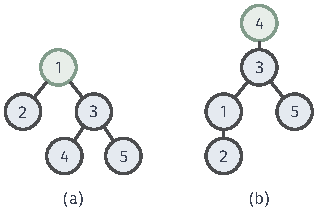
\includegraphics[scale=1]{figures/03-graphs/01-structure-and-computation/tikz/tree-root-choice/figure.pdf}
  \caption{同一棵树的两种选根。(a)以$1$为根，叶是$2,4,5$；(b)以$4$为根，叶是$2,5$。绿色顶点是根，边集不变，父子关系和有根树的叶集合随根改变。}
  \label{fig:graph-conn-tree-properties-roots}
\end{BookInlineFigure}

选根没有增删任何边，只规定每条边上哪一端是父节点；记录$n-1$个非根顶点的父节点就能还原边集，换一个根则全部重新确定。把每条边定向为从父节点指向子节点，得到一张有向图，但这一方向来自选根，而一般有向图的弧方向是原始数据，两者不应混同。第~\ref{sec:graph-tree-dp}节在有根树上自下而上计算时，利用的正是“每个子树只通过它的根与外界相连”。

\subsection{生成树与生成森林}
\label{sec:graph-conn-spanning-trees}

道路网中常要选出一部分道路，使所有城市仍然连通且没有多余的环，例如只维护最少的道路。所选的边必须取自原图，顶点则一个都不能少。

\begin{definition}[生成树与生成森林]
\label{def:graph-conn-spanning-tree}
设$\mathcal G=(V,E)$是无向图。若子图$(V,F)$，$F\subseteq E$，是一棵树，就称它为$\mathcal G$的\term{生成树}（spanning tree）。若$(V,F)$是森林，并且它的连通分量与$\mathcal G$的连通分量相同，就称它为$\mathcal G$的\term{生成森林}（spanning forest）。
\end{definition}

连通图一定有生成树，第~\ref{sec:graph-conn-tree-test}小节的构造选出的$(V,F)$就是一棵；只有连通图才有生成树。在每个分量上各取一棵生成树就得到生成森林，由式\eqref{eq:graph-conn-spanning-forest-edges}，它恰有$n-c$条边，其中$c$是原图的分量数。

\paragraph{生成树的核对与列举}
核对一个声称的生成树，只需检查$F\subseteq E$、$|F|=n-1$、$(V,F)$连通。贯穿图的$T_2$由$\{1,2\},\{1,3\},\{3,4\}$组成，三项都通过；三角形$\{1,2,3\}$的三条边也满足前两项，但没有连到顶点$4$。

同样的判定可以列举全部生成树。从$5$条边中选$3$条共$\binom53=10$种，有环的只有恰好选中三角形$\{1,2,3\}$或$\{2,3,4\}$的两种，所以生成树的个数是
\[
\binom53-2=10-2=8,
\]
见图~\ref{fig:graph-conn-spanning-trees}。

\begin{figure}[!htb]
  \centering
  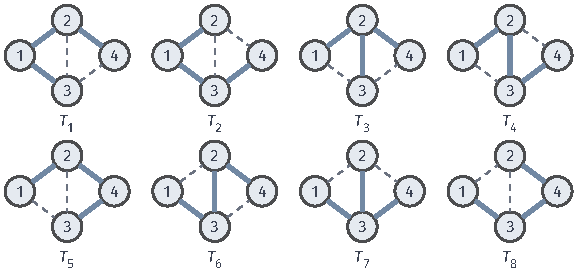
\includegraphics[width=97.652mm]{figures/01-basic-mathematics/04-graphs/tikz/c1-spanning-trees/figure.pdf}
  \caption{贯穿图的全部$8$棵生成树。蓝色粗线是树边，灰色虚线是被舍弃的原边。每棵生成树都有$3$条边并覆盖全部$4$个顶点；从$5$条边中选$3$条的$10$种选法里，只有恰好组成三角形$\{1,2,3\}$或$\{2,3,4\}$的两种不是树。}
  \label{fig:graph-conn-spanning-trees}
\end{figure}

生成树舍弃了环所提供的替代路径。以$T_2$为例：原图中$2,4$相邻，在$T_2$中却要经过$(2,1,3,4)$；原图没有割点，而$T_2$中$1$和$3$都成了割点。所以生成树上的距离和脆弱性一般不等于原图上的结果。生成森林恰好用最少的边给出第~\ref{sec:graph-conn-components}小节核对分量划分所需的块内连接。用遍历求生成森林是第~\ref{sec:graph-connectivity-computation}节的内容，它只保证连通、不比较边权；带建设成本时选总成本最小的一棵，是第~\ref{sec:graph-minimum-spanning-tree}章的问题。

\section{图的表示}
\label{sec:graph-representations}

要让计算机处理一张图，还得决定怎样存储它。不同的算法反复执行的操作不同：有的逐条扫描所有边，有的反复列出一个顶点的邻居，有的查询两个顶点之间是否有边，还有的做矩阵运算。选择记录方式时，要让这些反复执行的操作既正确又便宜。

本节介绍的四种常用表示各为一类操作而设计，图~\ref{fig:graph-conn-four-representations}把贯穿图的四种表示放在一起。比较时既看存储与访问的代价，也计入相互转换的代价；邻接矩阵还把行走计数变成矩阵乘法。代价用记号$O(\cdot)$表示：$O(g)$指操作次数或存储量不超过$g$的某个常数倍，常数与图的规模无关。这一记号描述的是规模增大时的增长速度，增长尺度的比较可参考\BookChapterRef{chap:limits-continuity}{第~\ref{chap:limits-continuity}章}。

\begin{figure}[!htb]
  \centering
  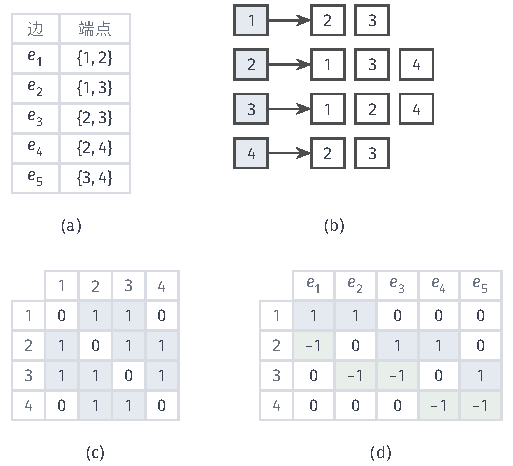
\includegraphics[width=89.524mm]{figures/01-basic-mathematics/04-graphs/tikz/c1-four-representations/figure.pdf}
  \caption{贯穿图的四种表示。(a)边列表逐条记录边的编号和端点；(b)邻接表为每个顶点（蓝色方框）列出邻居，每条无向边在两端各出现一次；(c)邻接矩阵按顶点次序记录每对顶点是否相邻，蓝色为$1$；(d)关联矩阵的每列对应一条边，按“小编号指向大编号”的记录方向，起点处为$1$（蓝色）、终点处为$-1$（绿色）。}
  \label{fig:graph-conn-four-representations}
\end{figure}

\subsection{边列表}
\label{sec:graph-conn-edge-list}

最直接的做法是把边一条条记下来。\term{边表}（edge list），也称边列表，为每条边保存一条记录：边的编号、两个端点，以及长度、容量等所需的属性。有向图的记录必须保存端点的次序。贯穿图的边列表见图~\ref{fig:graph-conn-four-representations}(a)，编号为$e_1=\{1,2\}$、$e_2=\{1,3\}$、$e_3=\{2,3\}$、$e_4=\{2,4\}$、$e_5=\{3,4\}$。有平行边时，两条边端点相同，只能靠编号区分。

边列表除顶点集外只需$O(m)$的存储，适合逐条处理全部边的算法，例如按边权排序（第~\ref{sec:graph-minimum-spanning-tree}章），或每一轮把每条边都检查一遍（第~\ref{sec:graph-shortest-paths}章）；求全部顶点的度也只需扫描一遍，即表~\ref{tab:graph-conn-degree-trace}的做法。它的弱点是查询局部信息：没有额外索引时，列出顶点$2$的邻居或判断$\{1,4\}$是否为边，都要扫描全部$m$条记录。

\subsection{邻接表}
\label{sec:graph-conn-adjacency-list}

遍历一张图时最频繁的操作是“列出当前顶点的全部邻居”，在边列表上每次都要扫描全部记录。\term{邻接表}（adjacency list）预先给每个顶点保存一个列表，列出它的邻居，需要时连同边的属性。无向边$\{i,j\}$在$i$和$j$的列表中各出现一次；有向图的邻接表默认只保存出邻居。

由边列表构造邻接表时，建立$n$个空列表，按编号扫描边列表：遇到无向边$\{i,j\}$，在$i$与$j$的列表末尾各追加对方；遇到弧$(i,j)$，只把$j$追加到$i$的列表。表~\ref{tab:graph-conn-adjacency-list-trace}是贯穿图上的构造过程，最后一行就是图~\ref{fig:graph-conn-four-representations}(b)。建表用$O(n)$时间，每条边追加两次，总共$O(n+m)$。

列表中邻居的次序取决于读边次序，第~\ref{chap:graph-traversal}章的遍历按列表次序读取邻居，所以执行过程会说明采用的次序。有向图若还要列出能一步到达$j$的顶点，就在读到$(i,j)$时再把$i$追加到$j$的入邻居列表，即反向图的出邻居表，存储增加$O(m)$。

\begin{table}[!htb]
  \centering
  \caption{由贯穿图的边列表构造邻接表。每读一条边，在两个端点的列表末尾各追加一项；最后一行即邻接表，各列表的长度依次是度$2,3,3,2$。}
  \label{tab:graph-conn-adjacency-list-trace}
  \small
  \begin{tabular}{@{}lccccc@{}}
    \toprule
    已读入的边 & 顶点$1$ & 顶点$2$ & 顶点$3$ & 顶点$4$ & 列表项总数\\
    \midrule
    初始 & 空 & 空 & 空 & 空 & $0$\\
    $e_1=\{1,2\}$ & $2$ & $1$ & 空 & 空 & $2$\\
    $e_2=\{1,3\}$ & $2,3$ & $1$ & $1$ & 空 & $4$\\
    $e_3=\{2,3\}$ & $2,3$ & $1,3$ & $1,2$ & 空 & $6$\\
    $e_4=\{2,4\}$ & $2,3$ & $1,3,4$ & $1,2$ & $2$ & $8$\\
    $e_5=\{3,4\}$ & $2,3$ & $1,3,4$ & $1,2,4$ & $2,3$ & $10$\\
    \bottomrule
  \end{tabular}
\end{table}

邻接表有$n$个列表头，无向图的列表项共$\sum_i d_i=2m$个（式\eqref{eq:graph-conn-handshake}），有向图的出邻居表共$m$个，所以存储量为$O(n+m)$。列出顶点$i$的邻居只需读它自己的列表，时间与$d_i$成正比；判断$\{i,j\}$是否为边则要在列表中查找，最坏需要$O(d_i)$时间。若一个算法对每个顶点恰好列出一次邻居，总工作量是$\sum_i(1+d_i)=n+2m$；第~\ref{chap:graph-traversal}章正是这样累计遍历的开销。

\subsection{邻接矩阵}
\label{sec:graph-conn-adjacency-matrix}

查询“$i,j$是否相邻”时，邻接表要在列表里查找。若预先给每一对顶点留一个位置，这个查询就能一步完成，代价是更多的存储；把这些位置排成方阵，还能直接使用矩阵运算。

固定顶点次序$1,\ldots,n$。无权图的\term{邻接矩阵}（adjacency matrix）$\bm A\in\mathbb R^{n\times n}$定义为
\begin{equation}
a_{i,j}=
\begin{cases}
1, & \{i,j\}\in E\ \text{（有向图中为}\ (i,j)\in E\text{）},\\
0, & \text{其他情形}.
\end{cases}
\label{eq:graph-conn-adjacency-matrix}
\end{equation}
带权时把有边位置的$1$换成边权$w_{i,j}$，记作$\bm W$。有向图采用“行是起点、列是终点”的约定。无向图的$\bm A$对称，有向图的邻接矩阵一般不对称。

构造时在全零矩阵上逐条填入边：无向边$\{i,j\}$令$a_{i,j}=a_{j,i}=1$，弧$(i,j)$只令$a_{i,j}=1$。贯穿图得到
\begin{equation}
\bm A=
\begin{bmatrix}
0&1&1&0\\
1&0&1&1\\
1&1&0&1\\
0&1&1&0
\end{bmatrix},
\label{eq:graph-conn-running-adjacency}
\end{equation}
第$i$行中为$1$的列号就是$N(i)$，行和就是度$2,3,3,2$，对角元为$0$对应没有自环。

有向图中行和是出度、列和是入度：$1\to2\leftarrow3$的邻接矩阵只有$a_{1,2}=a_{3,2}=1$，第$2$列读出$N^-(2)=\{1,3\}$，第$2$行全为$0$。

\paragraph{零权边与结构掩码}
在权矩阵$\bm W$中，零权边与无边都存成$0$，单看$\bm W$无法区分图~\ref{fig:graph-conn-zero-weight}(a)与(b)。允许零权边时要另存结构掩码$\bm M\in\{0,1\}^{n\times n}$，有边处为$1$。“是否相邻”查$\bm M$，“沿边累计多少”查$\bm W$；使用矩阵的算法应当说明它读的是哪一个。

\paragraph{稠密存储与稀疏存储}
存下全部$n^2$个条目称为稠密存储，查询一对顶点只需$O(1)$时间，列出一个顶点的邻居却要扫描整行，需要$O(n)$时间。

很多实际的图$m$远小于$n^2$：一个有$10^5$个路口的道路网，边数只是几十万量级，稠密邻接矩阵却需要$10^{10}$个条目。稀疏存储只保存非零条目，存储量为$O(n+m)$，按行访问时与邻接表相当。所以说一个算法的代价时必须同时说明存储方式：邻接表上为$O(n+m)$的遍历，搬到稠密矩阵上就变成$O(n^2)$。

\subsection{邻接矩阵的幂与行走计数}
\label{sec:graph-conn-adjacency-powers}

从$1$到$4$走两步有几种走法？走三步回到原处有几种？这类计数在传播过程中反复出现，逐条列举很快变得繁琐。图写成矩阵后，它们可以用矩阵乘法回答；所用的只是乘积的逐项定义$(\bm X\bm Y)_{i,j}=\sum_\ell x_{i,\ell}y_{\ell,j}$，矩阵运算的一般规则可参考\BookChapterRef{chap:linear-operations}{第~\ref{chap:linear-operations}章}。

先看长度为$2$的情形。按乘积的定义，
\[
(\bm A^2)_{i,j}=\sum_{\ell}a_{i,\ell}a_{\ell,j},
\]
而$a_{i,\ell}a_{\ell,j}=1$当且仅当$(i,\ell,j)$是一条长度为$2$的行走。所以对中间顶点$\ell$求和，数出的正是从$i$到$j$长度为$2$的行走条数。这一观察可以推广到任意长度。

\begin{theorem}[邻接矩阵的幂计数行走]
\label{thm:graph-conn-adjacency-powers}
设$\bm A$是无权图（无向或有向）的邻接矩阵，$k\geq0$为整数。则对任意顶点$i,j$，
\begin{equation}
(\bm A^k)_{i,j}=\#\{\text{从}\ i\ \text{到}\ j\ \text{长度为}\ k\ \text{的行走}\}.
\label{eq:graph-conn-adjacency-power-walks}
\end{equation}
\end{theorem}

\begin{proof}
对$k$归纳。$k=0$时$\bm A^0=\bm I$，长度为零的行走只有停在原地的$(i)$。设结论对$k$成立。从$i$到$j$长度为$k+1$的行走按倒数第二个顶点$\ell$分类：它由一条从$i$到$\ell$长度为$k$的行走接上一步$\ell\to j$组成，这一步存在当且仅当$a_{\ell,j}=1$。每条行走恰好落入一类，所以
\[
\#\{\text{从}\ i\ \text{到}\ j\ \text{长度为}\ k+1\ \text{的行走}\}
=\sum_{\ell=1}^{n}(\bm A^k)_{i,\ell}\,a_{\ell,j}
=(\bm A^{k+1})_{i,j}.
\]
\end{proof}

无向图中$(\bm A^2)_{i,j}$就是$i$与$j$的公共邻居个数（$i=j$时是$i$的度）。贯穿图得到
\[
\bm A^2=
\begin{bmatrix}
2&1&1&2\\
1&3&2&1\\
1&2&3&1\\
2&1&1&2
\end{bmatrix}.
\]

图~\ref{fig:graph-conn-adjacency-square}说明了其中第$(1,4)$个条目的来历。按中间顶点求和时只有$\ell=2,3$两项非零，
\[
(\bm A^2)_{1,4}=a_{1,2}a_{2,4}+a_{1,3}a_{3,4}=2,
\]
对应$(1,2,4)$与$(1,3,4)$。对角元$d_i$数的是走到一个邻居再立刻返回的闭行走，它们不是环。

再乘一次$\bm A$可以数三角形。对角元按乘法定义展开为
\[
(\bm A^3)_{i,i}=\sum_j(\bm A^2)_{i,j}a_{j,i},
\]
即对$i$的邻居$j$累加$(\bm A^2)_{i,j}$。贯穿图得对角元$2,4,4,2$，迹为$12$。长度为$3$的闭行走中三个顶点两两相邻，恰好组成一个三角形，而每个三角形可以从$3$个顶点出发、沿$2$个方向绕行，所以三角形个数为
\[
\frac{\operatorname{tr}(\bm A^3)}{6}=\frac{12}{6}=2.
\]

\begin{figure}[!htb]
  \centering
  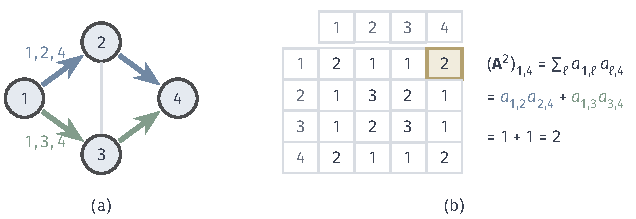
\includegraphics[width=110.352mm]{figures/01-basic-mathematics/04-graphs/tikz/c1-adjacency-square-walks/figure.pdf}
  \caption{邻接矩阵的平方计数长度为$2$的行走。(a)从$1$到$4$的两条行走$(1,2,4)$（蓝色）与$(1,3,4)$（绿色），中间顶点分别是$2$和$3$；(b)贯穿图的$\bm A^2$，黄色条目$(\bm A^2)_{1,4}=2$按中间顶点$\ell$求和，只有$\ell=2,3$的两项非零。}
  \label{fig:graph-conn-adjacency-square}
\end{figure}

\paragraph{计数的范围与代价}
这个计数包含重复顶点的行走，不能直接当作路径数或环数；更长的闭行走会混入往返与重复绕行，不能像三角形那样简单换算。

矩阵幂也能判断可达，但代价很高。由引理~\ref{lem:graph-conn-walk-contains-path}，$j$从$i$可达当且仅当$\bm I+\bm A+\cdots+\bm A^{n-1}$的第$(i,j)$个条目为正，但每次稠密乘法要$n^3$次乘加，远高于遍历的$O(n+m)$；矩阵幂的价值在于计数和代数性质。

带权时$(\bm W^k)_{i,j}$是行走上边权乘积之和，既不是条数也不是长度之和；沿路线相加再取最小，需要把乘法换成加法、求和换成取最小，属于第~\ref{sec:graph-shortest-paths}章。

\subsection{关联矩阵}
\label{sec:graph-conn-incidence-matrix}

邻接矩阵以顶点对为单位，看不出“第几条边”。以边为单位的计算，例如对每条边比较两个端点上的数值，需要行对应顶点、列对应边的矩阵。把边编号为$e_1,\ldots,e_m$，给每条无向边任选一个记录方向，例如把$e_k=\{i,j\}$记为从$i$到$j$。\term{关联矩阵}（incidence matrix）$\bm B\in\mathbb R^{n\times m}$的第$k$列在起点$i$处为$1$、终点$j$处为$-1$，其余为$0$；有向图直接用弧的方向。

构造时按编号读边列表，在第$k$列的起点行写$1$、终点行写$-1$。贯穿图取“小编号指向大编号”的记录方向，得到
\begin{equation}
\bm B=
\begin{bmatrix}
1&1&0&0&0\\
-1&0&1&1&0\\
0&-1&-1&0&1\\
0&0&0&-1&-1
\end{bmatrix},
\label{eq:graph-conn-running-incidence}
\end{equation}
即图~\ref{fig:graph-conn-four-representations}(d)。每列恰有两个非零元且和为$0$，第$i$行的非零元个数等于度$d_i$；不满足这两条的列就是记错的边。

对无向图，记录方向只是一种约定。反转第$k$条边的记录方向，第$k$列整列变号，相当于右乘一个对角元为$\pm1$的对角矩阵，图本身没有改变，所以反映图性质的计算不应依赖这一选择。有向图的弧方向则是数据的一部分。

关联矩阵的列以边为单位，正适合以边为单位的计算。若给每个顶点赋一个数，组成向量$\bm x\in\mathbb R^n$，则$\bm B^{\top}\bm x$的第$k$个分量是
\[
(\bm B^{\top}\bm x)_k=\sum_v b_{v,k}x_v=x_i-x_j,
\]
即第$k$条边记录的起点与终点上数值之差。反转这条边的记录方向只改变差的符号，不改变差的大小。顶点与边上的数值函数、由$\bm B$构造的拉普拉斯矩阵及加权度，可参考\BookChapterRef{chap:graph-functions-operators}{第~\ref{chap:graph-functions-operators}章}。

\subsection{四种表示的比较}
\label{sec:graph-conn-representation-comparison}

表~\ref{tab:graph-conn-representation-costs}汇总了前面各小节的分析。没有一种表示在所有操作上都最好：逐边处理用边列表，逐点列邻居用邻接表，频繁查询顶点对或做矩阵运算用邻接矩阵，以边为单位的线性计算用关联矩阵。

\begin{table}[!htb]
  \centering\small
  \begin{tabular}{@{}lcccc@{}}
    \toprule
    表示 & 存储 & 扫描全部边 & 列出$i$的邻居 & 查询$\{i,j\}$是否为边\\
    \midrule
    边列表 & $O(n+m)$ & $O(m)$ & $O(m)$ & $O(m)$\\
    邻接表 & $O(n+m)$ & $O(n+m)$ & $O(d_i)$ & $O(d_i)$\\
    稠密邻接矩阵 & $O(n^2)$ & $O(n^2)$ & $O(n)$ & $O(1)$\\
    稠密关联矩阵 & $O(nm)$ & $O(nm)$ & $O(m+d_in)$ & $O(m)$\\
    \bottomrule
  \end{tabular}
  \caption{四种表示的存储与三种基本访问的时间代价，$n$为顶点数，$m$为边数，$d_i$为顶点$i$的度。边列表、邻接表不附加索引；稠密关联矩阵列出邻居时先扫描第$i$行找出$d_i$条邻边，再在每条边的列中找另一个端点。关联矩阵若改用按行、按列都可访问的稀疏存储，存储降为$O(n+m)$，列出邻居的代价与邻接表相当。}
  \label{tab:graph-conn-representation-costs}
\end{table}

算法所需的表示往往与输入不同，转换的代价也应计入：边列表与邻接表互转用$O(n+m)$时间；由边列表建稠密邻接矩阵要$O(n^2+m)$，由稠密邻接矩阵建邻接表要读遍$n^2$个条目；建稠密关联矩阵仅置零就要$O(nm)$。

选择表示时，先列出算法反复执行的操作，再按表估计总代价并计入转换与存储：第~\ref{chap:graph-traversal}章的遍历用邻接表，第~\ref{chap:minimum-spanning-tree}章按边权排序用边列表，图上的矩阵算子则用邻接矩阵与关联矩阵。实际程序常同时保存两种表示，额外的存储也应计入。

\section{图同构}
\label{sec:graph-isomorphism}

顶点的名称只是为了区分顶点而取的。把贯穿图的顶点换一套编号，边集的写法会变，邻接矩阵的行列也会移动，连接结构本身却没有变。本节用保持邻接的一一对应把“只差一套名称”写成同构的定义。

有了定义，给定的对应容易核对，不同构也常能用简单的量排除，难的是在没有给出对应时断定同构。最后一小节用置换矩阵把重编号写成矩阵运算。系统比较两张图结构的算法是第~\ref{sec:graph-wl-refinement}节的内容。

\subsection{图同构的定义}
\label{sec:graph-conn-isomorphism-definition}

图~\ref{fig:graph-conn-isomorphism}(a)是贯穿图$\mathcal G$；(c)的$\mathcal G'$顶点集也是$\{1,2,3,4\}$，边集由$\{1,3\}$、$\{1,4\}$、$\{2,3\}$、$\{2,4\}$、$\{3,4\}$组成，两者的边集不相等。但若按(b)的规则$\rho$把$\mathcal G$的顶点改名，$\mathcal G$的五条边依次变为下面五个无序对：
\[
\begin{gathered}
\{1,2\}\mapsto\{1,3\},\qquad
\{1,3\}\mapsto\{1,4\},\qquad
\{2,3\}\mapsto\{3,4\},\\
\{2,4\}\mapsto\{3,2\},\qquad
\{3,4\}\mapsto\{4,2\}.
\end{gathered}
\]
它们恰好是$\mathcal G'$的全部边；唯一不相邻的一对$\{1,4\}$变为$\{1,2\}$，在$\mathcal G'$中也不相邻。可见这样的改名要一一对应，并且相邻的仍相邻，不相邻的仍不相邻。

\begin{figure}[!htb]
  \centering
  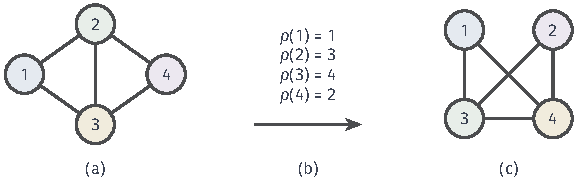
\includegraphics[width=97.688mm]{figures/01-basic-mathematics/04-graphs/tikz/c1-isomorphism-relabeling/figure.pdf}
  \caption{两张同构的图。(a)贯穿图$\mathcal G$；(c)画法与编号都不同的$\mathcal G'$；(b)顶点对应$\rho$。同色顶点互相对应：$\mathcal G$中顶点$i$与$\mathcal G'$中顶点$\rho(i)$颜色相同。逐条核对可见，$\mathcal G$中相邻的顶点对恰好对应$\mathcal G'$中相邻的顶点对。}
  \label{fig:graph-conn-isomorphism}
\end{figure}

\begin{definition}[图同构]
\label{def:graph-conn-isomorphism}
设$\mathcal G=(V,E)$与$\mathcal G'=(V',E')$是无向图。若存在双射$\rho:V\to V'$，使对任意$i,j\in V$都有
\[
\{i,j\}\in E\iff\{\rho(i),\rho(j)\}\in E',
\]
就称$\mathcal G$与$\mathcal G'$\term{同构}（isomorphic），称$\rho$为一个同构映射。
\end{definition}

双向条件不能减弱为单向：边集为$\{1,2\},\{2,3\}$的路径按恒等映射放进三角形$\{1,2,3\}$，边都映为边，但三角形多出了边$\{1,3\}$。反方向的条件保证$\mathcal G'$中不出现多余的连接。

有向图的同构要求$(i,j)\in E\iff(\rho(i),\rho(j))\in E'$。$1\to2\to3$与$1\to2\leftarrow3$的底层无向图相同，作为有向图却不同构：同构映射保持入度，而后者的顶点$2$入度为$2$。加权图还要求$w'_{\rho(i),\rho(j)}=w_{i,j}$；带属性的图要由问题声明哪些属性必须保持，例如顶点带有类别时，可以要求同构映射只把顶点映到同类顶点。

\subsection{同构的核对与排除}
\label{sec:graph-conn-isomorphism-checking}

若别人给出了一个对应$\rho$，只需核对它是否满足定义；若只给出两张图，则要判断是否存在这样的对应，后者困难得多。

\paragraph{给定对应的核对}
定义的条件要对全部$\binom n2$个顶点对检查。下面的引理说明，只需检查边的像，再比较边数。

\begin{lemma}[同构映射的核对]
\label{lem:graph-conn-isomorphism-check}
设$\rho:V\to V'$是双射，$|E|=|E'|$，并且$\mathcal G$的每条边$\{i,j\}$都满足$\{\rho(i),\rho(j)\}\in E'$。则$\rho$是$\mathcal G$到$\mathcal G'$的同构映射。
\end{lemma}

\begin{proof}
由于$\rho$是单射，$\{i,j\}\mapsto\{\rho(i),\rho(j)\}$是从$E$到$E'$的单射；两个有限集合元素个数相同，所以它是双射。于是若$\{\rho(i),\rho(j)\}\in E'$，它是某条边$\{i',j'\}\in E$的像，由$\rho$单射得$\{i',j'\}=\{i,j\}\in E$。
\end{proof}

本节开头的例子正是这样核对的：$\rho$是双射，两图都有$5$条边，五条边的像都在$E'$中，所以$\rho$是同构映射，“不相邻的一对仍不相邻”这一步可以省去。$\mathcal G'$以邻接矩阵存储时，核对用$O(n+m)$时间。

\paragraph{图不变量}
同构映射保持一切由连接结构定义的量：顶点数、边数、每个顶点的度（$\rho$把$i$的邻居一一映为$\rho(i)$的邻居）、度的多重集合、连通分量个数、三角形个数等。这些量称为\term{图不变量}（graph invariant），只要有一个不同，两张图就不同构；计算时宜从便宜的顶点数、边数和排序后的度开始。

例如，六个顶点排成的环与两个互不相连的三角形，顶点数、边数都是$6$，每个顶点的度都是$2$，但前者连通、后者有两个分量，所以不同构。

反过来，比较过的不变量都相同，也不足以断定同构。考虑两棵六个顶点的树，边集分别为
\[
\bigl\{\{1,2\},\{1,3\},\{1,4\},\{2,5\},\{3,6\}\bigr\}
\quad\text{与}\quad
\bigl\{\{1,2\},\{1,3\},\{1,4\},\{2,5\},\{5,6\}\bigr\}.
\]
二者都连通、没有三角形，度的多重集合都是$\{3,2,2,1,1,1\}$。但前一棵树中度为$3$的顶点$1$与两个度为$2$的顶点$2,3$相邻，后一棵树中顶点$1$只与一个度为$2$的顶点$2$相邻。同构映射必须保持度为$3$的顶点及其邻居的度，所以两棵树不同构：比较“邻居的度”能区分只看度区分不了的图。

要得出“同构”的肯定结论，必须真的找到一个对应。逐个尝试全部$n!$个双射再逐个核对，虽然总能判定，但$n=20$时$n!$已超过$2\times10^{18}$。不变量可以缩小搜索，例如度为$3$的顶点只能映到度为$3$的顶点。第~\ref{sec:graph-wl-refinement}节的顶点标记细化把“比较邻居的度”反复执行，并会说明它仍然不能区分所有不同构的图。

\subsection{重编号与置换表示}
\label{sec:graph-conn-relabeling}

当两张图的顶点集都是$\{1,\ldots,n\}$时，同构映射$\rho$就是一个重编号。重编号以后，邻接矩阵的行和列都要按同样的方式重排，置换矩阵恰好执行这种重排，于是同构可以直接在矩阵上核对。

记$\bm e_i$为第$i$个分量为$1$、其余分量为$0$的标准基向量。取置换矩阵$\bm P=\begin{bmatrix}\bm e_{\rho(1)}&\cdots&\bm e_{\rho(n)}\end{bmatrix}$，即第$i$列是$\bm e_{\rho(i)}$，它满足$\bm P\bm e_i=\bm e_{\rho(i)}$。按条目写，$p_{k,i}=1$当且仅当$k=\rho(i)$，其余条目为$0$；由于$\rho$是双射，$\bm P$的每行、每列都恰有一个$1$。

计算$\bm P\bm A\bm P^{\top}$的条目时，按乘法定义展开
\[
(\bm P\bm A\bm P^{\top})_{k,l}=\sum_{i=1}^{n}\sum_{j=1}^{n}p_{k,i}\,a_{i,j}\,p_{l,j}.
\]
求和中只有$k=\rho(i)$且$l=\rho(j)$的一项非零，所以左乘$\bm P$把第$i$行移到第$\rho(i)$行，右乘$\bm P^{\top}$把第$j$列移到第$\rho(j)$列。两者合起来，
\begin{equation}
\bm A'=\bm P\bm A\bm P^{\top},\qquad
a'_{\rho(i),\rho(j)}=a_{i,j}.
\label{eq:graph-conn-relabel}
\end{equation}
原来记录“$i,j$是否相邻”的条目被搬到了新编号的位置。因此，$\rho$是$\mathcal G$到$\mathcal G'$的同构映射，当且仅当$\mathcal G'$的邻接矩阵等于$\bm P\bm A\bm P^{\top}$。

对图~\ref{fig:graph-conn-isomorphism}的$\rho$，$\bm P$的各列依次为$\bm e_1,\bm e_3,\bm e_4,\bm e_2$，即
\[
\bm P=
\begin{bmatrix}
1&0&0&0\\
0&0&0&1\\
0&1&0&0\\
0&0&1&0
\end{bmatrix}.
\]
再取式\eqref{eq:graph-conn-running-adjacency}的$\bm A$，计算得
\[
\bm P\bm A\bm P^{\top}=
\begin{bmatrix}
0&0&1&1\\
0&0&1&1\\
1&1&0&1\\
1&1&1&0
\end{bmatrix}.
\]
这个矩阵的第$1$行读出$N'(1)=\{3,4\}$，第$4$行读出$N'(4)=\{1,2,3\}$，各行都与$\mathcal G'$的边集一致；例如$a'_{3,2}=a'_{\rho(2),\rho(4)}=a_{2,4}=1$。

实际计算不必做矩阵乘法，按第二式把每个条目搬到$(\rho(i),\rho(j))$即可，代价为$O(n^2)$。加权图同样要求$\bm W'=\bm P\bm W\bm P^{\top}$；允许零权边时还要检验结构掩码$\bm M'=\bm P\bm M\bm P^{\top}$。

\paragraph{置换与一般换基}
$\bm P$的各列是互不相同的标准基向量，所以$\bm P^{\top}\bm P=\bm I$，即$\bm P^{\top}=\bm P^{-1}$。于是式\eqref{eq:graph-conn-relabel}可以写成$\bm A'=\bm P\bm A\bm P^{-1}$，是一个相似变换，即在另一组基下表示同一个线性映射（可参考\BookChapterRef{chap:linear-representation}{第~\ref{chap:linear-representation}章}）。

但反过来，一般的相似变换不能都解释为重编号。对两个顶点一条边的图，$\bm A=\left[\begin{smallmatrix}0&1\\1&0\end{smallmatrix}\right]$，取$\bm S=\left[\begin{smallmatrix}1&1\\0&1\end{smallmatrix}\right]$，其逆为$\bm S^{-1}=\left[\begin{smallmatrix}1&-1\\0&1\end{smallmatrix}\right]$。先左乘$\bm S$，
\[
\bm S\bm A
=\begin{bmatrix}1&1\\0&1\end{bmatrix}
\begin{bmatrix}0&1\\1&0\end{bmatrix}
=\begin{bmatrix}1&1\\1&0\end{bmatrix};
\]
再右乘$\bm S^{-1}$，得到
\[
\bm S\bm A\bm S^{-1}
=\begin{bmatrix}1&1\\1&0\end{bmatrix}
\begin{bmatrix}1&-1\\0&1\end{bmatrix}
=\begin{bmatrix}1&0\\1&-1\end{bmatrix}.
\]
这个矩阵不对称，有非零对角元和负条目，不是任何简单无向图的邻接矩阵。一般换基混合不同顶点的坐标，重编号只搬动位置。

相似变换保持特征值，所以邻接矩阵的特征值也是图不变量：特征值不同的两张图一定不同构。但它和其他不变量一样只能排除同构，特征值相同的两张图未必同构。

\section{本章小结}
\label{sec:graph-objects-summary}

本章开头问：图记录了什么，沿连接能到哪里，删除连接会怎样，结构又怎样记录和比较。第一个问题的回答是，图$\mathcal G=(V,E)$只记录有限个对象之间的直接连接，与纸上的画法无关，比较两幅画只需比较顶点集与边集。方向、边权和属性各自附加一类信息。方向决定哪些顶点序列可以通行，忽略方向得到的底层无向图丢掉了先后。边权的含义由问题决定：长度沿路线相加，容量限制单条边的通过量，相似度鼓励两端接近；零权边仍是边，“能否到达”查边集，“累计多少”查边权。子图可以任意保留一部分边，诱导子图则保留选定顶点之间的全部边，因而由顶点集唯一确定。

沿连接能到哪里，由行走和路径回答。行走允许重复，便于拼接与计数；路径不重复顶点，对应实际路线。任何行走都可以随读随删地化成一条同端点的路径，所以用两者定义的可达关系相同。无向图中可达关系是等价关系，它把顶点集唯一地划分为连通分量；核对一个声称的划分，只需检查没有边跨越不同的块、每块内部连通。有向图中可达不对称，要区分要求双向到达的强连通与忽略方向的弱连通，前者蕴含后者，反之不然。任务能否排出先后，取决于有没有顺着箭头绕回起点的有向环；不含有向环的有向无环图，底层无向图仍可以有环。

删除连接的影响由分隔集、割点和桥刻画，判断的依据始终是有没有替代路径。核对分隔集，就是在删除后的图中求出可达集；一条边是桥当且仅当它不在任何环上，删边至多使分量数增加一，删点却可能把分量拆成许多块。用最少的边保持连通，就得到树：树等价于任意两点之间路径唯一，$n$个顶点的树恰有$n-1$条边。连通、无环、恰有$n-1$条边三个条件中任意两个推出第三个，所以判断树只需数边再查连通。选根把树组织成父子层次而不改变边集；生成森林在每个分量上保留一棵生成树，恰有$n-c$条边，并且一般不唯一，它丢掉了原图的替代路径。

同一张图可以用边列表、邻接表、邻接矩阵和关联矩阵记录。四者保存的连接相同，支持的访问和代价不同，转换本身也有代价，选择时应先列出算法反复执行的操作。邻接矩阵还把组合计数变成矩阵运算：$\bm A^k$的条目计数长度为$k$的行走，其中包含重复顶点，不能直接当作路径数。

同构用保持邻接与不相邻的双射刻画“只差一套名称”，在矩阵上表现为置换共轭$\bm A'=\bm P\bm A\bm P^{\top}$。给定对应时，核对边的像并比较边数就够了。度、分量数、特征值等不变量可以排除同构，却不足以确认同构，而逐个尝试$n!$个对应并不可行。

本章说明了怎样在小图上核对连通分量、强连通分量、生成树、无环性和同构，却还没有给出在大图上高效求出它们的方法。第~\ref{chap:graph-traversal}章在邻接表上用广度优先和深度优先遍历实际计算这些对象，用拓扑排序安排有向无环图的次序，并用顶点标记细化比较图的结构；那里的算法输出，仍要按本章的定义与核对方法检验。


\chapter{图的遍历与结构计算}
\label{chap:graph-traversal}

第~\ref{chap:graph-objects}章定义了可达、连通分量、强连通分量、有向无环图、分隔集和同构。这些定义说明了什么样的结构算数，却没有说明怎样在一张存放在计算机里的图上把它们找出来。例如，可达性要求“存在一条路径”，而路径数目可以随顶点数指数增长，逐条列举并不可行。本章只沿邻接关系有组织地访问顶点，由此得到距离、分量和依赖次序，并说明每项输出为什么正确、花费多少计算。

第~\ref{sec:graph-bfs}节和第~\ref{sec:graph-dfs}节给出两种基本的访问方式，后面各节都以它们为工具。广度优先遍历用队列由近及远逐层推进，得到最少边数和相应路线；深度优先遍历用栈沿一条分支走到底再退回，得到发现与完成两种次序，并能判断有没有环。

其余四节把两种遍历用于第~\ref{chap:graph-objects}章的各个结构。第~\ref{sec:graph-connectivity-computation}节计算无向连通分量和生成森林，引入在不断加边时维护分量的并查集，再用两遍深度优先遍历求出有向图的强连通分量；把每个强分量缩成一点，得到的图没有有向环。第~\ref{sec:graph-topological-order}节在无环图上安排依赖次序。第~\ref{sec:graph-separator-blocks}节删除一个给定的顶点集，把图拆成若干共享接口的局部块。第~\ref{sec:graph-wl-refinement}节回到同构问题，用邻域信息反复细化顶点标记，得到不依赖编号的比较手段，并指出它的局限。

本章讨论有限图，输入以第~\ref{sec:graph-conn-adjacency-list}小节的邻接表给出，默认无自环、无平行边，需要保留边身份时另行说明。记顶点数为$n=|V|$，无向图的边数和有向图的弧数都记为$m$；邻接表中无向边在两端各存一次，有向图默认只存出邻居。复杂度中的$O(n+m)$表示所需基本操作次数不超过$n+m$的常数倍。

本章的算法只使用结构上的邻接，不比较边权：生成森林只要求连通、不要求总权最小，广度优先遍历只数边数、不计长度。在给定结构中寻找最小成本或最大流量，是第~\ref{part:graph-combinatorial-optimization}部分的问题。

\section{广度优先遍历}
\label{sec:graph-bfs}

给定一张图和一个起点，最基本的问题是：从起点出发能走到哪些顶点，走到每个顶点最少要经过几条边，又该沿哪条路线走。广度优先遍历按离起点的远近逐层访问顶点，一次就回答这三个问题。

\subsection{问题与思路}
\label{sec:graph-trav-bfs-problem}

输入是图$\mathcal G=(V,E)$的邻接表和一个起点$s\in V$。记$\operatorname{dist}(s,v)$为从$s$到$v$的路径所含的最少边数，有向图中路径沿弧的方向；$v$从$s$不可达时约定$\operatorname{dist}(s,v)=+\infty$。对每个顶点$v$，我们要知道它是否从$s$可达；若可达，$\operatorname{dist}(s,v)$是多少，以及一条恰好用$\operatorname{dist}(s,v)$条边从$s$走到$v$的路线。

按定义逐条检查路径是行不通的。从$s$到$v$的路径可能极多，而且路径越长，种类增长越快；即使只想知道最少边数，也不能把所有路径列出来再比较。

不枚举路径，可以按距离把顶点分层。距离为$0$的只有$s$自己，距离为$1$的恰好是$s$的邻居。距离为$2$的顶点不在前两层，却与第$1$层某个顶点相邻：从$s$走两条边能到达它，一条边到不了。一般地，前$k$层找全以后，第$k+1$层就是与第$k$层相邻、但还没出现过的顶点。于是从第$0$层开始，每次由当前层找出下一层，直到某一层为空。

一个顶点可能与上一层的多个顶点相邻，也可能与本层或更早的顶点相邻，所以它只能在第一次被找到时归入某一层，之后再遇到就跳过。找到它时顺手记下是从哪个顶点找到的，沿这些记录往回走，就能恢复一条路线。

\subsection{算法实现}
\label{sec:graph-trav-bfs-algorithm}

逐层推进不必真的维护一层层的列表，一个先进先出的队列就够了：先进入队列的顶点先展开，第$k$层的顶点全部展开完之前，第$k+1$层的顶点只在队尾排队。算法维护四项状态：
\begin{itemize}
  \item 发现标记：顶点是否已经被找到；
  \item 队列$Q$：已经发现、但邻居尚未检查的顶点；
  \item 边数距离$d(v)$：$v$被找到时所在的层号；
  \item \term{父指针}（parent pointer）$p(v)$：$v$是在展开哪个顶点时第一次被找到的。
\end{itemize}
初始时只有$s$被发现，$d(s)=0$，$p(s)$为空，$Q=[s]$；其余顶点未发现，$d(v)=+\infty$。

此后每一轮从队首取出一个顶点$u$，依次检查它的邻居。未发现的邻居$v$属于$u$的下一层：立即把它标记为已发现，写入$d(v)=d(u)+1$和$p(v)=u$，放到队尾。已发现的邻居则跳过。

队列变空时，从$s$可达的顶点都已找到。这种按层访问的过程称为广度优先遍历，也常称\term{广度优先搜索}（breadth-first search，BFS）。

\begin{algorithm}[广度优先遍历]
\label{alg:graph-trav-bfs}
输入：图$\mathcal G=(V,E)$的邻接表，起点$s\in V$。输出：距离$d(v)$与父指针$p(v)$，$v\in V$。
\begin{enumerate}
  \item 标记$s$为已发现，置$d(s)=0$、$p(s)$为空，令$Q=[s]$；其余顶点未发现，$d(v)=+\infty$。
  \item 当$Q$非空时，取出队首$u$，按邻接表依次读取$u$的邻居$v$（有向图只读出邻居$v\in N^+(u)$）。若$v$未发现，立即标记$v$为已发现，置$d(v)=d(u)+1$、$p(v)=u$，并把$v$放到队尾；若$v$已发现，跳过。
  \item 队列为空时停止。
\end{enumerate}
\end{algorithm}

要让每个顶点只在第一次被找到时归入某一层，必须在它入队时就做标记。两个已发现的顶点可能共享一个尚未发现的邻居；若等到出队时才标记，这个邻居会被两个顶点各放入队列一次，距离和父指针也可能被改写。入队即标记，每个顶点就至多入队一次。

\paragraph{执行过程}
在第~\ref{sec:graph-basic-concepts}节的贯穿四点图上，以$1$为起点，并约定按编号从小到大读取邻居。图~\ref{fig:graph-trav-bfs-queue}(b)逐行列出了每次出队后的队列。初始$Q=[1]$，此后四轮依次为：
\begin{itemize}
  \item 取出$1$：发现$2,3$，写入$d(2)=d(3)=1$、$p(2)=p(3)=1$，队列变为$[2,3]$。
  \item 取出$2$：邻居$1,3$都已发现，只有$4$是新的，写入$d(4)=2$、$p(4)=2$，队列变为$[3,4]$。
  \item 取出$3$：邻居$1,2,4$全部已发现，$4$不会第二次入队，队列变为$[4]$。
  \item 取出$4$：没有新顶点，队列为空，算法停止。
\end{itemize}
图~\ref{fig:graph-trav-bfs-queue}(a)把各顶点按$d$值分到三层，蓝色箭头就是父指针所指的边。

\begin{figure}[!htb]
  \centering
  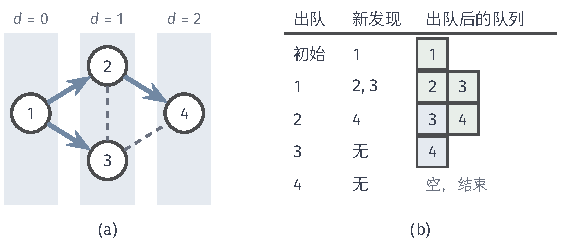
\includegraphics[width=106.7mm]{figures/01-basic-mathematics/04-graphs/tikz/c2-bfs-queue-trace/figure.pdf}
  \caption{贯穿四点图上从顶点$1$出发的广度优先遍历，邻居按编号递增读取。(a)顶点按边数距离$d$分为三层，蓝色箭头是父指针对应的边，虚线是检查过但没有带来新顶点的边。(b)每次出队后的队列，队首在左，绿色格子是这一步新入队的顶点；取出$3$时$4$已在队中，不再重复入队。}
  \label{fig:graph-trav-bfs-queue}
\end{figure}

\paragraph{路线的恢复}
要得到从$s$到已发现顶点$t$的路线，从$t$出发反复取父指针，直到回到$s$，再把得到的顶点序列反转。父指针总是指向更早发现的顶点，所以回溯不会绕圈，一定在有限步内回到$s$。

在上例中，$4$的父指针是$2$，$2$的父指针是$1$，反转后得到路线$1\to2\to4$，恰有$d(4)=2$条边。若$t$始终未被发现，即$d(t)=+\infty$，算法应报告$t$从$s$不可达，而不能输出任何路线。

路线并不唯一。若改为先读$3$再读$2$，取出$1$后队列为$[3,2]$，$4$在展开$3$时被发现，父指针变成$p(4)=3$，路线变成$1\to3\to4$。两条路线不同，边数却都是$2$：改变同层顶点的处理次序可能改变父指针，但下面的定理表明它不改变距离。

\subsection{算法分析}
\label{sec:graph-trav-bfs-correctness}

\paragraph{正确性}
算法只在顶点第一次被发现时写入$d(v)$，以后不再修改。正确性的关键在于，这个“第一次”恰好发生在最短的距离上。

\begin{theorem}[广度优先遍历的距离]
\label{thm:graph-trav-bfs-distance}
设对有限图$\mathcal G$和起点$s$执行算法~\ref{alg:graph-trav-bfs}。则对每个顶点$v$，$d(v)=\operatorname{dist}(s,v)$；当$v$可达时，沿父指针从$v$回到$s$的路线恰有$d(v)$条边。
\end{theorem}

\begin{proof}
先说明$d(v)$不会小于真实距离。若$d(v)$有限且$v\neq s$，则$d(p(v))=d(v)-1$，沿父指针每退一步距离减一，$d(v)$步后回到$s$。反转这串顶点就得到一条从$s$到$v$、恰有$d(v)$条边的路线，所以$d(v)\geq\operatorname{dist}(s,v)$。

再说明队列中的距离值有一个固定的形状：从队首到队尾不减，且最大值与最小值至多相差$1$。初始队列只有$s$，满足这一点。设某时刻队列中的值为若干个$k$后接若干个$k+1$，取出的队首$u$有$d(u)=k$，新加入的顶点距离都是$k+1$，并放在队尾，形状仍然保持。由此可知，顶点出队时的距离值按时间不减。

最后对$\delta=\operatorname{dist}(s,v)$归纳，证明有限距离的顶点都会被发现且$d(v)\leq\delta$。$\delta=0$时$v=s$。设$\delta\geq1$，并设距离小于$\delta$的顶点都已满足结论。取一条从$s$到$v$的最短路径，记其倒数第二个顶点为$x$，则$\operatorname{dist}(s,x)=\delta-1$，由归纳假设$x$被发现且$d(x)=\delta-1$。

$x$入过队，就一定在某一时刻出队并检查邻居$v$。若此时$v$尚未发现，就得到
\[
d(v)=d(x)+1=\delta;
\]
若$v$已经被发现，则发现它的顶点$u$出队不晚于$x$，按上一段的单调性$d(u)\leq d(x)$，于是
\[
d(v)=d(u)+1\leq d(x)+1=\delta.
\]

两个方向合起来得到$d(v)=\operatorname{dist}(s,v)$。不可达的顶点没有任何从$s$出发的路线，第一段说明它不可能得到有限的$d$值。
\end{proof}

证明第二段的队列形状把“逐层推进”变成了可以检验的事实：处理第$k$层时只会首次发现第$k+1$层的顶点，而它们全部排在第$k$层之后。最短路径上的倒数第二个顶点$x$比$v$少一层，一定先被展开，所以$v$不会拖到更远的层才被发现。

\paragraph{复杂度}
以邻接表存储时，每个顶点至多入队、出队各一次，出队时把它的邻接表读一遍，因此每条邻接记录只被检查常数次。无向图的邻接记录共$2m$条，有向图的出邻接记录共$m$条，总时间为$O(n+m)$。发现标记、距离、父指针和队列各占$O(n)$额外空间。

这一结论依赖“列出邻居的代价与度数成正比”。若改用邻接矩阵，找出一个顶点的邻居要扫描一整行，$n$个顶点共扫描$n^2$个位置，时间变为$O(n^2)$；对稀疏图，这比$O(n+m)$大得多。

\paragraph{适用范围}
广度优先遍历把每条边都算作一步，而边上带有长度时，边数最少的路线不一定总长度最小。图~\ref{fig:graph-trav-bfs-weighted}中，从$s$直接到$t$只需一条边，广度优先遍历就用这条边记录$t$，但它的长度是$5$；经过$a$的路线多走一条边，总长度却只有$1+1=2$。所以广度优先遍历只解决所有边长相等时的最短路问题。一般边长下的最短路需要比较累计长度，留到第~\ref{sec:graph-shortest-paths}章。

\begin{figure}[!htb]
  \centering
  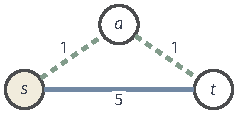
\includegraphics[width=87.8mm]{figures/01-basic-mathematics/04-graphs/tikz/c2-bfs-weighted-counterexample/figure.pdf}
  \caption{带权反例。边旁数字是长度。广度优先遍历从$s$出发时经直接边一步发现$t$（蓝色），这条路线总长$5$；绿色虚线路线$s\text{--}a\text{--}t$多一条边，总长只有$2$。广度优先遍历最小化的是边数，不是总长度。}
  \label{fig:graph-trav-bfs-weighted}
\end{figure}

一次广度优先遍历也只覆盖从$s$可达的部分。遍历结束时距离仍为$+\infty$的顶点没有被访问，不能据此断言它们是孤立点，它们之间可能有很多边。要给全图的每个顶点划分连通分量，需要在外层不断换新的起点重新启动，这是第~\ref{sec:graph-connectivity-computation}节的内容。

\subsection{多源广度优先遍历}
\label{sec:graph-trav-multi-source-bfs}

有时关心的不是离某一个起点多远，而是离一组起点中最近的那个多远。例如在网格上放置若干个种子，问每个格子离最近的种子几步。给定起点集合$S\subseteq V$，要求的是
\begin{equation}
\operatorname{dist}(S,v)=\min_{s\in S}\operatorname{dist}(s,v),
\label{eq:graph-trav-multi-source-dist}
\end{equation}
空集上的最小值约定为$+\infty$；同时还想知道$v$离哪个起点最近。

既然只关心最近的起点，就把$S$中的所有顶点一起当作第$0$层，从这一层开始逐层推进。实现上只改初始化：$S$中所有顶点都标记为已发现、距离为$0$、父指针为空，并按任意次序全部放入队列；此后的更新与算法~\ref{alg:graph-trav-bfs}完全相同。这称为\term{多源广度优先遍历}（multi-source breadth-first search）。

它的正确性可以归结到单源情形。设想添加一个新顶点$s^*$，从它向$S$中每个顶点连一条边（有向图中连弧$s^*\to s$）。因为从$s^*$出发的路线第一步必然进入$S$，新图中任一原顶点$v$满足
\[
\operatorname{dist}(s^*,v)=1+\operatorname{dist}(S,v).
\]
从$s^*$做普通广度优先遍历，第一次出队就把$S$中所有顶点以距离$1$放入队列，此后的过程与多源版本完全相同，只是所有距离多了$1$。

把定理~\ref{thm:graph-trav-bfs-distance}用于新图，再减去多出的$1$，可知多源版本输出$\operatorname{dist}(S,v)$。沿父指针回溯会停在某个起点上，回溯路线恰有$\operatorname{dist}(S,v)$条边，所以这个起点就是离$v$最近的起点之一。

图~\ref{fig:graph-trav-multi-source}是一个$3\times5$网格，相邻格子以上下左右相连，中间一个格子不属于图。两个起点放在左上角和右下角，每个格子中的数字是它到较近起点的边数。例如第一行第四个格子离左上角$3$步、离右下角也是$3$步，记为$3$，两个起点都是它的最近起点；第一行最右的格子离右下角只有$2$步，记为$2$。若只从左上角出发，右下角的格子距离为$6$。

\begin{figure}[!htb]
  \centering
  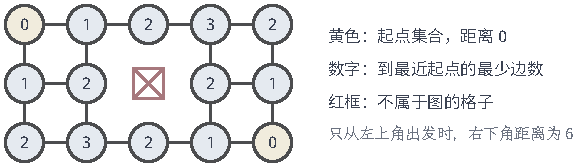
\includegraphics[width=99.0mm]{figures/01-basic-mathematics/04-graphs/tikz/c2-multi-source-bfs/figure.pdf}
  \caption{$3\times5$网格上的多源广度优先遍历。网格以上下左右相邻连边，红框格子不属于图；两个黄色起点同时作为第$0$层。每个顶点中的数字是到较近起点的最少边数，所有距离由一次遍历得到。}
  \label{fig:graph-trav-multi-source}
\end{figure}

对每个起点各做一次广度优先遍历，回答的是另一个问题：它得到$|S|$组距离，能说出$v$到每个起点各有多远，需要$O(|S|(n+m))$时间。多源遍历只给出到最近起点的距离及对应的起点，一次只需$O(n+m)$时间。若$S$为空，队列一开始就为空，所有顶点保持未发现，与$\operatorname{dist}(\varnothing,v)=+\infty$的约定一致。

\paragraph{来源标签的同步传播}
逐个回溯父指针才能知道来源，每次要花与距离成正比的时间。若需要全部顶点的最近来源，可以让来源随发现一起传下去。为此再维护一个数组$\operatorname{src}(\cdot)$，它的初始化与更新规则是：
\begin{itemize}
  \item 初始化时，对每个$s\in S$置$\operatorname{src}(s)=s$；
  \item 展开$u$时每发现一个新顶点$v$，除写入$d(v)$和$p(v)$外，再置$\operatorname{src}(v)=\operatorname{src}(u)$。
\end{itemize}

由于$p(v)=u$，按父指针归纳可知$\operatorname{src}(v)$就是从$v$回溯父指针到达的起点，所以它是$v$的一个最近来源。离两个起点一样近的顶点（例如上面网格第一行第四个格子）只记录先发现它的那一个；需要全部最近来源时，要在距离相等的情形下另行合并记录。

\section{深度优先遍历}
\label{sec:graph-dfs}

广度优先遍历同时推进许多条路线，每条只走一步。深度优先遍历只盯住一条路线往前走，走到无路可走再退回来。它同样能找出全部可达顶点，还额外记录了当前正沿哪条分支前进、某个顶点之后的部分何时全部探完；后面判断有向环、计算强连通分量和安排依赖次序，都要用到这两项信息。

\subsection{问题与思路}
\label{sec:graph-trav-dfs-idea}

输入仍是图$\mathcal G=(V,E)$的邻接表。我们要访问全部顶点，并对每个顶点记录三项信息：它是从哪个顶点走过来的，即父指针$p(v)$；它何时第一次被走到；它何时被彻底处理完，即从它出发能继续探索的部分何时全部探完。后两项用一个逐步递增的时钟记录，分别称为发现时刻$d(v)$和完成时刻$f(v)$。广度优先遍历给出的距离回答“离起点多远”，却不回答“谁的后续先探完”这类先后问题。

做法是一条路走到底再回头：从当前顶点挑一个还没去过的邻居走过去，再从那里继续往前；到了一个顶点，若它的邻居都已去过或者根本没有邻居，就退回上一个顶点，改走它的下一个邻居。退回到起点、起点也没有可走的邻居时，从起点能到达的部分就探完了。走迷宫时扶着一侧墙一路前进、碰到死路再折回，就是这种方式。

\paragraph{环的处理}
如果不记录哪些顶点已经去过，“一直往前走”在有环的图上会停不下来。图~\ref{fig:graph-trav-dfs-idea}(a)中，弧为$1\to2$、$2\to3$、$3\to1$、$3\to4$。从$1$出发沿弧前进，走到$3$后若选择$3\to1$，就回到了起点，接着又走$1\to2\to3$，如此绕圈，永远不会检查$4$，也永远不会结束。

所以要给顶点加上发现标记，并规定只走向尚未发现的邻居：遇到已经发现的邻居就不进入，接着看下一个邻居；当前顶点的邻居都检查完了，就回头。图~\ref{fig:graph-trav-dfs-idea}(b)中，走到$3$时看到$1$已发现，不进入，改走$4$；$4$没有出邻居，回头到$3$；$3$的邻居检查完毕，再依次回头到$2$、$1$。每个顶点只被走进一次，绕圈就不可能发生。

\begin{figure}[!htb]
  \centering
  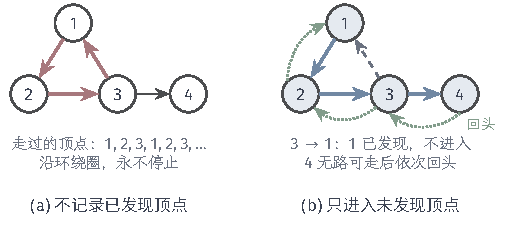
\includegraphics[width=84.748mm]{figures/01-basic-mathematics/04-graphs/tikz/c2-dfs-backtrack-idea/figure.pdf}
  \caption{深度优先遍历的回头规则。有向图的弧为$1\to2$、$2\to3$、$3\to1$、$3\to4$。(a)不记录已发现的顶点时，沿红色的环反复前进，永远到不了$4$；(b)只走向未发现的顶点：蓝色是实际走过的弧，虚线弧$3\to1$因$1$已发现而不进入；$4$无路可走后沿绿色点线依次回头。}
  \label{fig:graph-trav-dfs-idea}
\end{figure}

\paragraph{回头所需的记录}
回头还带来两个要求。第一，退回到某个顶点时，要接着检查它的下一个邻居，而不是从头再来，所以每个顶点要记住自己的邻居检查到了哪里。

第二，“已发现”要再细分：一个顶点被走到之后、邻居检查完之前，它位于从起点到当前位置的这条分支上；邻居全部检查完后，它就离开了分支，不会再从它出发。前者称为处理中，后者称为已完成，加上尚未被走到的未发现，顶点共有三种状态。处理中的顶点恰好构成当前分支，判断环时要用到这一点（第~\ref{sec:graph-trav-cycle-detection}小节）；完成时刻则记录了某个顶点之后的部分何时全部探完。

\subsection{算法实现}
\label{sec:graph-trav-dfs-stack}

当前分支后进先出，最后走到的顶点最先退回，所以用一个栈保存它：栈底是本次起点，栈顶是当前顶点。算法维护五项状态：
\begin{itemize}
  \item 顶点状态：每个顶点是未发现、处理中还是已完成；
  \item 栈$S$：当前分支上的顶点，每一帧$(u,\text{位置})$记录顶点$u$以及$u$的邻接表中下一条待检查记录的位置；
  \item 父指针$p(v)$：$v$是从哪个顶点第一次走到的；
  \item 发现时刻$d(v)$与完成时刻$f(v)$：$v$进栈和出栈时的时钟读数；
  \item 时钟$t$：到目前为止发生过的发现与完成事件的次数。
\end{itemize}

初始时所有顶点都是未发现，栈为空，$t=0$。从起点$r$出发时，令$p(r)$为空，时钟加一后记为$d(r)$，$r$改为处理中，压入帧$(r,\text{邻接表起点})$。

此后每一步只看栈顶帧$(u,\text{位置})$，按$u$的邻居是否已经检查完，分为前进和回头两种情形：
\begin{itemize}
  \item 前进：$u$还有未检查的邻居。读出下一个邻居$v$，把位置后移一格。若$v$未发现，就走到$v$：置$p(v)=u$，时钟加一后记为$d(v)$，$v$改为处理中，压入帧$(v,\text{邻接表起点})$。若$v$已发现，不进入，这一步结束。
  \item 回头：$u$的邻居已全部检查。时钟加一后记为$f(u)$，$u$改为已完成，弹出栈顶帧，下一步回到它下面的顶点。
\end{itemize}

栈变空时，从$r$可达的部分已经探完。这种访问方式称为深度优先遍历，也常称\term{深度优先搜索}（depth-first search，DFS）。

\begin{algorithm}[深度优先遍历（显式栈）]
\label{alg:graph-trav-dfs}
输入：图$\mathcal G=(V,E)$的邻接表。输出：父指针、每个顶点的发现时刻$d(v)$与完成时刻$f(v)$。
\begin{enumerate}
  \item 所有顶点置为未发现，时钟$t=0$。按某个固定次序扫描顶点；每遇到一个未发现的顶点$r$，令$p(r)$为空，执行下面两步。
  \item 发现$r$：$t\gets t+1$，$d(r)=t$，$r$改为处理中，把帧$(r,\text{邻接表起点})$压入栈。
  \item 当栈非空时，看栈顶帧$(u,\text{位置})$。若$u$还有未检查的邻居，读取下一个邻居$v$（有向图只读出邻居），并把位置后移一格：$v$未发现时，置$p(v)=u$，$t\gets t+1$，$d(v)=t$，$v$改为处理中并压入新帧；$v$处于处理中或已完成时，不压栈，继续下一轮。若$u$的邻居已全部检查，则$t\gets t+1$，$f(u)=t$，$u$改为已完成并弹出栈顶帧。
\end{enumerate}
\end{algorithm}

第一步的外层扫描保证覆盖全部顶点：栈空时若仍有未发现的顶点，就从下一个未发现顶点重新开始，已经完成的顶点不会被重新访问。

父指针把顶点组织成若干棵有根树，每次重新开始产生一棵，合起来称为深度优先森林。

\paragraph{执行过程}
图~\ref{fig:graph-trav-dfs-stack}是一个有分支的有向图，弧为$1\to2$、$1\to5$、$2\to3$、$2\to4$、$5\to4$。从$1$出发并按编号读取出邻居。
\begin{BookInlineFigure}
  \centering
  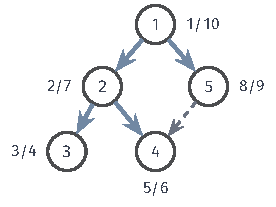
\includegraphics[width=46.655mm]{figures/03-graphs/01-structure-and-computation/tikz/reading-steps/dfs-input-graph.pdf}
  \caption{深度优先遍历的算例。顶点旁的“$d/f$”是下文计算出的发现时刻与完成时刻；蓝色箭头是父指针对应的弧，虚线弧$5\to4$检查时$4$已完成。}
  \label{fig:graph-trav-dfs-stack}
\end{BookInlineFigure}

十个事件依次为：
\begin{enumerate}
  \item 发现$1$，$d(1)=1$，栈为$[1]$。
  \item $1$的第一个出邻居$2$未发现，前进，$d(2)=2$，栈为$[1,2]$。
  \item $2$的第一个出邻居$3$未发现，前进，$d(3)=3$，栈为$[1,2,3]$。
  \item $3$没有出邻居，回头：$f(3)=4$，弹出$3$。
  \item 回到$2$，它的下一个出邻居$4$未发现，前进，$d(4)=5$。
  \item $4$也没有出邻居，$f(4)=6$，弹出。
  \item 此时$2$的邻居已检查完，$f(2)=7$，弹出。
  \item 回到$1$，下一个出邻居$5$未发现，前进，$d(5)=8$。
  \item $5$唯一的出邻居$4$已经完成，不进入，$5$的邻居随即检查完，$f(5)=9$。
  \item 最后$f(1)=10$，栈变空。
\end{enumerate}
图~\ref{fig:graph-trav-dfs-stack-events}画出了每个事件之后的栈，黄色格子是栈顶。
\begin{BookInlineFigure}
  \centering
  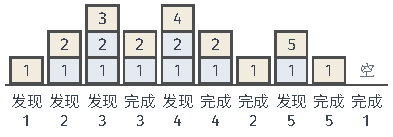
\includegraphics[width=66.622mm]{figures/03-graphs/01-structure-and-computation/tikz/reading-steps/dfs-stack-events.pdf}
  \caption{十个事件之后的栈。栈底在下，栈顶为黄色；栈高上升对应发现，下降对应完成。完成$2$后回到$1$，随后才进入分支$5$。}
  \label{fig:graph-trav-dfs-stack-events}
\end{BookInlineFigure}



\subsection{算法分析}
\label{sec:graph-trav-dfs-orders}

\paragraph{发现次序与完成次序}
按发现时刻从小到大排列顶点，得到\term{发现次序}（discovery order）；按完成时刻排列，得到\term{完成次序}（finishing order）。在图~\ref{fig:graph-trav-dfs-stack}中，发现次序是$1,2,3,4,5$，完成次序是$3,4,2,5,1$。

两者的差别来自栈的结构：一个顶点被发现之后、弹栈之前压入的所有顶点都位于它上方，必须先弹出。所以一个顶点的后代全部先于它完成；$2$的后代$3,4$先完成，然后才轮到$2$。下面两个引理把这一观察写准确，本节的正确性论证以及后面的强连通分量和拓扑排序都要用到它们。

\begin{lemma}[时刻区间的嵌套]
\label{lem:graph-trav-dfs-nesting}
在一次完整的深度优先遍历中，若顶点$v$在$u$处于处理中时被发现，即$d(u)<d(v)<f(u)$，则$v$是$u$在深度优先森林中的后代，且$f(v)<f(u)$。
\end{lemma}

\begin{proof}
$v$被发现时压入栈，位于$u$的上方，因为此时$u$仍在栈中。栈后进先出，$v$必须在$u$之前弹出，所以$f(v)<f(u)$。另外，$v$的父指针指向发现它时的栈顶，这个栈顶要么是$u$，要么是在$u$之后压入的顶点；对后者重复同样的推理，父指针链只会经过$u$上方的顶点，最终到达$u$。因此$v$是$u$的后代。
\end{proof}

图~\ref{fig:graph-dfs-time-intervals}把同一次遍历的发现和完成时刻画成区间。顶点$2$的区间包含$3,4$的区间，而$2$与$5$的区间不相交；这种包含与分离直接反映了深度优先森林中的祖先关系。

\begin{figure}[!htb]
  \centering
  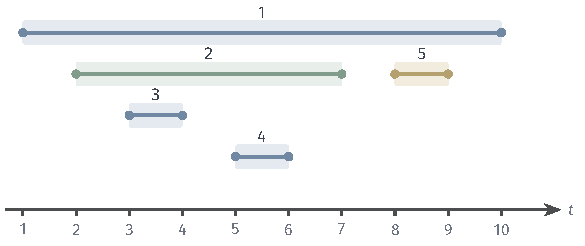
\includegraphics[width=98.986mm]{figures/03-graphs/01-structure-and-computation/tikz/dfs-time-intervals/figure.pdf}
  \caption{深度优先遍历的时间区间。沿用图~\ref{fig:graph-trav-dfs-stack}的图和邻居次序；每条横段从$d(v)$延伸到$f(v)$，段上数字为顶点编号。后代的区间严格嵌入祖先的区间，不同分支的区间互不相交。}
  \label{fig:graph-dfs-time-intervals}
\end{figure}

\begin{lemma}[未发现路径]
\label{lem:graph-trav-white-path}
若在时刻$d(u)$存在一条从$u$到$v$的路径（有向图中沿弧方向），路径上除$u$以外的顶点此时都未发现，则$v$最终成为$u$的后代，从而$f(v)<f(u)$。
\end{lemma}

\begin{proof}
假设结论不成立，在路径上取第一个不成为$u$后代的顶点$w$，记它在路径上的前一个顶点为$x$。$x$是$u$本身或$u$的后代，所以$f(x)\leq f(u)$。$x$在完成之前要检查弧$x\to w$，因此$w$在$f(x)$之前已被发现；而按假设$w$在$d(u)$时尚未发现，所以$d(u)<d(w)<f(x)\leq f(u)$。由引理~\ref{lem:graph-trav-dfs-nesting}，$w$是$u$的后代，矛盾。
\end{proof}

\paragraph{正确性}
回头规则保证了不重复：只有未发现的顶点才会压栈，压栈的同时它就变为处理中，此后不可能再次压栈，所以每个顶点恰好被发现一次、完成一次，环不会让算法反复进入同一个顶点。每一帧的位置只向后移动，每条邻接记录至多读一次，栈的每次变化不是压入一个新顶点就是弹出一个顶点，所以算法一定在有限步内停止。

也不会遗漏。设$r$是第一次扫描到的起点，在时刻$d(r)$其余顶点都未发现，任何从$r$可达的顶点都通过一条全由未发现顶点组成的路径与$r$相连。由引理~\ref{lem:graph-trav-white-path}，它们都成为$r$的后代，即在从$r$出发的这一次遍历中被访问。外层扫描又保证每个顶点最终都会被发现。所以一次完整的遍历把全部顶点恰好访问一次，从单个起点出发时访问的恰是它的可达集。

\paragraph{复杂度}
每个顶点恰好压栈、弹栈各一次，每条邻接记录恰好被读取一次，所以邻接表下总时间为$O(n+m)$，状态、时刻、父指针和栈占$O(n)$额外空间。栈的深度等于当前分支上的顶点数，最坏可达$n$：在一条长链$1\to2\to\cdots\to n$上，栈会一直增长到装下全部顶点。

\paragraph{与广度优先遍历的比较}
两种遍历访问的顶点集合相同，代价也同为$O(n+m)$，记录的结构却不同，不能互相替代。

深度优先遍历的父指针也给出从根到每个顶点的路线，但它反映的是沿哪条分支先走到，与距离无关。在贯穿四点图上从$1$出发、按编号读取邻居：$1$走到$2$，$2$的第一个未发现邻居是$3$，$3$的未发现邻居是$4$，于是父路径为$1\to2\to3\to4$，有三条边；而$1\to2\to4$只需两条边，$1$与$3$甚至直接相邻。需要最少边数时，应使用广度优先遍历。

反过来，完成次序是广度优先遍历给不出的信息，也不能用发现次序代替。设图~\ref{fig:graph-trav-dfs-stack}中的弧表示依赖，$i\to j$意味着$i$要排在$j$之前。顶点$4$同时是$2$和$5$的后继。若按发现次序$1,2,3,4,5$安排，$5$排在$4$之后，违反了弧$5\to4$：发现$4$时走的是经过$2$的分支，发现次序没有反映$5$也指向它。

完成次序则不同：$4$在$5$之前就已完成，反转完成次序得到$1,5,2,4,3$，五条弧都是起点在前。第~\ref{sec:graph-trav-dfs-toposort}小节会证明，在无环图中这一做法总是成立。

\subsection{环的检测}
\label{sec:graph-trav-cycle-detection}

给定一张图，我们要判断它是否含有环；若有，还要输出一个具体的环，使人可以逐条边核对。有向环意味着依赖关系自相矛盾，无法排出先后；无向图中的环意味着图不是森林。遍历中“遇到已发现的邻居就不进入”正是环留下的痕迹，但并非每次遇到已发现的邻居都说明有环，需要按顶点状态分清楚。

\paragraph{有向图}
处理中的顶点构成当前分支，父指针已经把它们按先后串成一条有向路径。若检查栈顶$u$的出邻居时遇到弧$u\to v$，而$v$也处于处理中，那么沿父指针从$u$往回走一定会到达$v$，这段路径与弧$u\to v$合起来就是一个有向环。这样的弧称为\term{回边}（back edge）。

图~\ref{fig:graph-trav-cycle-detection}(a)中，栈内依次是$1,2,3$，检查$3\to1$时$1$仍在栈中，沿父指针$3\to2\to1$回溯，再补上$3\to1$，得到有向环$1\to2\to3\to1$。图~\ref{fig:graph-trav-dfs-idea}(b)中被跳过的弧$3\to1$正是这样一条回边。

指向已完成顶点的弧则不同。图~\ref{fig:graph-trav-cycle-detection}(b)中先走$1\to2$，$2$没有出邻居而完成；回到$1$后走到$3$，检查$3\to2$时$2$已完成。$2$已经不在当前分支上，弧$3\to2$无法与当前分支拼成环。本例中从$2$出发也回不到$3$（否则由引理~\ref{lem:graph-trav-white-path}，$3$会在$2$完成之前就被发现），图中确实没有环。只看“是否已经访问过”会把这种情形误判为环，这就是要区分处理中与已完成的原因。

\begin{figure}[!htb]
  \centering
  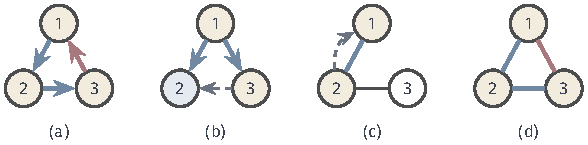
\includegraphics[width=99.369mm]{figures/01-basic-mathematics/04-graphs/tikz/c2-dfs-cycle-detection/figure.pdf}
  \caption{深度优先遍历中环的判断。黄色为处理中（在栈内）的顶点，蓝色填充为已完成顶点，蓝色粗线为父指针对应的边。(a)有向图中$3\to1$指向栈内顶点，构成回边，沿父指针恢复出环；(b)$3\to2$指向已完成顶点，不构成环；(c)无向图中从$2$回看父边$\{1,2\}$，这是同一条边的反向查看，应当跳过；(d)无向三角形中$3$遇到已发现、但不经父边相连的顶点$1$，构成环（红色）。}
  \label{fig:graph-trav-cycle-detection}
\end{figure}

\begin{theorem}[有向环的判定]
\label{thm:graph-trav-directed-cycle}
有限有向图含有向环，当且仅当对它的一次完整深度优先遍历中出现回边。出现回边$u\to v$时，父指针链$v\to\cdots\to u$加上弧$u\to v$就是一个有向环。
\end{theorem}

\begin{proof}
充分性已在上面说明：$v$处于处理中且$u$是当前栈顶，$u$在$v$上方，由引理~\ref{lem:graph-trav-dfs-nesting}$u$是$v$的后代，父指针链给出从$v$到$u$的有向路径。

必要性。设图含有向环，在环上取最先被发现的顶点$v$，记环上指向$v$的弧为$u\to v$。在时刻$d(v)$，环上其余顶点都未发现，沿环从$v$走到$u$的路径满足引理~\ref{lem:graph-trav-white-path}的条件，所以$u$成为$v$的后代，$d(v)<d(u)<f(u)<f(v)$。$u$在完成之前要检查弧$u\to v$，那时$v$尚未完成，仍处于处理中，因此$u\to v$是一条回边。
\end{proof}

因此判断有向环只需在算法~\ref{alg:graph-trav-dfs}的第三步多做一次检查：读到的邻居$v$处于处理中时，报告回边并沿父指针取出环。时间仍为$O(n+m)$。

\paragraph{无向图}
无向图中每条边在两端的邻接表里各出现一次。从$u$走到$v$之后，$v$检查邻居时会再次看到$u$，这只是同一条边的反向记录，不是新的路线。若把它当作“遇到已发现顶点”，任何一条边都会被误判为环，如图~\ref{fig:graph-trav-cycle-detection}(c)。因此规则是：检查$u$的一条邻接记录$e=\{u,w\}$时，若$e$就是使$u$被发现的父边，跳过；否则只要$w$已经被发现，就报告存在环。

图~\ref{fig:graph-trav-cycle-detection}(d)中，$3$经父边与$2$相连，它看到的$1$已被发现、且不经父边相连，于是$1\text{--}2\text{--}3\text{--}1$是一个环。允许平行边时，要按边的身份跳过，只跳过实际作为父边的那一条；两点之间的另一条平行边会与父边构成长度为$2$的环。

这一规则在两个方向上都可靠。先看没有报告的情形。若整次遍历从未报告，每条边在两端被检查时，要么发现了新顶点而成为父边，要么正是父边的反向记录，所以所有边都是父边，图就是深度优先森林本身，没有环。

再看报告的情形。考察第一次报告时的边$e=\{u,w\}$，此时$u$在栈顶、处于处理中，下面说明$w$也在栈中。假设$w$已完成，那么$w$在完成之前已经从自己一端检查过$e$。若那时$u$未发现，$w$会经$e$发现$u$，$u$成为$w$的子节点并先于$w$完成，与$u$此刻仍在处理中相矛盾。若那时$u$已发现，那次检查本身就该报告，除非$e$是$w$的父边；而$e$是$w$的父边意味着$u$当初正是读$e$这条记录发现了$w$，每条记录只读一次，$u$不会现在再读到它。两种情形都不可能，所以$w$在栈中，是位于$u$下方的祖先。

于是父指针链从$w$到$u$再加上$e$构成一个环。在简单图中，若$w$是$u$的父节点，父边只能是$e$本身，而$e$不是$u$的父边；所以这条父指针链至少有两条边，环至少有三个顶点。算法因此既给出“有环”的结论，也给出可以直接核对的环本身。

\section{连通结构的计算}
\label{sec:graph-connectivity-computation}

第~\ref{sec:graph-connectivity-separation}节按相互可达把顶点划分为连通分量或强连通分量，那是存在性的定义。本节把它们算出来，处理三个相关的问题：无向图的连通分量，边不断加入时无向图的连通分量，以及有向图的强连通分量。三个问题的任务相同，都是给每个顶点$v$打上一个分量标签$\operatorname{comp}(v)$，使两个顶点标签相同当且仅当它们属于同一个分量。有了标签，“$u$与$v$是否连通”就变成比较两个数是否相等，不必再去找路径。

三种做法都从遍历出发，差别来自图的形态。无向图上可达关系是对称的，一次遍历恰好找出一个分量，只需在外面套一层扫描；边逐条加入时，分量只会合并，需要一种能快速合并标签的数据结构；有向图上从一个顶点能到达的范围往往大于与它相互可达的范围，一次遍历不再恰好停在分量边界上，需要借助深度优先遍历的完成次序。

\subsection{无向图的连通分量}
\label{sec:graph-trav-components-forest}

\subsubsection{问题与思路}

输入是无向图$\mathcal G=(V,E)$的邻接表。要输出每个顶点的分量标签$\operatorname{comp}(v)\in\{1,\ldots,c\}$和分量个数$c$，使得$\operatorname{comp}(u)=\operatorname{comp}(v)$当且仅当$u$与$v$之间有路径。

从顶点$r$出发做一次广度或深度优先遍历，找到的是从$r$可达的全部顶点。无向图中可达关系是对称的，所以这些顶点恰好就是与$r$在同一分量的顶点，不多也不少。给它们打上同一个新标签，一个分量就处理完了。剩下的顶点里若还有没打标签的，它一定属于另一个分量，再从它出发遍历一次。于是在外面套一层扫描，依次从尚未打标签的顶点启动遍历，每启动一次就得到一个分量。

\subsubsection{算法实现}

算法在所用遍历的状态之外，只多维护两项：
\begin{itemize}
  \item 标签数组$\operatorname{comp}(\cdot)$：每个顶点所属分量的编号，$0$表示尚未标记；它同时充当遍历的发现标记，$\operatorname{comp}(v)\neq0$就表示$v$已发现；
  \item 已用的标签个数$c$。
\end{itemize}
初始时$\operatorname{comp}$全为$0$，$c=0$。外层扫描每遇到一个$\operatorname{comp}(r)=0$的顶点，就令$c\gets c+1$并从$r$启动遍历；遍历中每发现一个新顶点$v$，就写入$\operatorname{comp}(v)=c$。

\begin{algorithm}[无向连通分量编号]
\label{alg:graph-trav-components}
输入：无向图的邻接表。输出：每个顶点的分量编号$\operatorname{comp}(v)$，以及分量数$c$。
\begin{enumerate}
  \item 所有顶点置$\operatorname{comp}(v)=0$，$c=0$。
  \item 按任意固定次序扫描顶点。遇到$\operatorname{comp}(r)=0$的顶点$r$时，令$c\gets c+1$，从$r$启动一次广度（或深度）优先遍历，把这次新发现的每个顶点$v$标记为$\operatorname{comp}(v)=c$。已经标记的顶点不再作为起点，也不清除旧编号。
  \item 扫描完全部顶点后输出。
\end{enumerate}
\end{algorithm}

\paragraph{执行过程}
图~\ref{fig:graph-trav-components-forest}中的图由贯穿四点图、一条边$\{5,6\}$和孤立点$7$组成。按编号扫描、每次启动广度优先遍历，标签数组的变化如表~\ref{tab:graph-trav-components-trace}所示。外层扫描依次经过：
\begin{itemize}
  \item 扫描到$1$：它尚未标记，令$c=1$，从$1$出发的遍历标出$\{1,2,3,4\}$。
  \item 扫描到$2,3,4$：它们已有标签，跳过。
  \item 扫描到$5$：令$c=2$，遍历标出$\{5,6\}$。
  \item 扫描到$6$：已有标签，跳过。
  \item 扫描到$7$：它没有任何邻居，但外层扫描仍会遇到它，令$c=3$，它自成一个分量。
\end{itemize}

\begin{table}[!htb]
  \centering
  \small
  \begin{tabular}{@{}lcccccccc@{}}
    \toprule
    扫描到的起点 & $c$ & $1$ & $2$ & $3$ & $4$ & $5$ & $6$ & $7$ \\
    \midrule
    初始 & $0$ & $0$ & $0$ & $0$ & $0$ & $0$ & $0$ & $0$ \\
    $1$ & $1$ & $1$ & $1$ & $1$ & $1$ & $0$ & $0$ & $0$ \\
    $5$ & $2$ & $1$ & $1$ & $1$ & $1$ & $2$ & $2$ & $0$ \\
    $7$ & $3$ & $1$ & $1$ & $1$ & $1$ & $2$ & $2$ & $3$ \\
    \bottomrule
  \end{tabular}
  \caption{按编号扫描时标签数组$\operatorname{comp}$的变化。只列出启动遍历的三次扫描，其余扫描遇到已标记的顶点而跳过；“$0$”表示尚未标记。}
  \label{tab:graph-trav-components-trace}
\end{table}

\subsubsection{算法分析}

\paragraph{正确性}
每次启动的遍历恰好标出一个完整的分量。由第~\ref{sec:graph-bfs}节的分析，从$r$出发的遍历找到从$r$可达的全部顶点；无向图中可达就是同在一个分量，所以这次遍历标出的恰是$r$所在的分量。它不会碰到先前已标记的顶点，因为那些顶点属于别的分量，与$r$之间没有路径。

外层扫描必须覆盖全部顶点，否则没有边的孤立点不会被任何遍历发现，也就得不到标签。改变扫描次序，例如先扫描$7$，标签的数值会变，哪些顶点被分到一起却不会变，因为分量本身由图决定。

\paragraph{复杂度}
各次遍历访问的顶点互不重叠，合起来每个顶点被发现一次，每条邻接记录被读常数次；外层扫描本身读$n$个标签。总时间为$O(n+m)$，标签数组和遍历所需的队列或栈占$O(n)$额外空间。给全图所有顶点打标签，与从一个起点做一次遍历同阶。

\subsubsection{生成森林}
\label{sec:graph-trav-spanning-forest}

标签只说明哪些顶点连在一起，遍历过程还顺带留下了它们连在一起的证据。每个新顶点都是经某条边第一次被发现的；把这些父边$\{p(v),v\}$全部保留，遇到已发现顶点的边一律不加，就得到原图的一个生成森林，不需要额外计算。

\begin{theorem}[发现父边构成生成森林]
\label{thm:graph-trav-parent-forest}
设对无向图$\mathcal G$执行算法~\ref{alg:graph-trav-components}，并保留所有父边。则这些父边与全部顶点组成$\mathcal G$的一个生成森林，它在每个分量上是一棵生成树，边数为$n-c$。
\end{theorem}

\begin{proof}
每个非起点顶点恰有一条父边，父边的另一端是更早发现的顶点；起点没有父边。于是父边共$n-c$条。

再说明父边不成环。假设某些父边构成一个环，取环上最晚发现的顶点$v$。$v$在环上有两条边，另两端都比$v$早发现。但与$v$相连的父边中，只有$v$自己的父边通向更早发现的顶点，其余父边都是$v$的子顶点的父边，另一端比$v$晚发现。矛盾。

最后，每次遍历从起点出发，沿父指针可以从任何新发现的顶点回到起点，所以每个分量内的父边是连通的。连通、无环、覆盖分量的全部顶点，就是该分量的生成树。
\end{proof}

\begin{figure}[!htb]
  \centering
  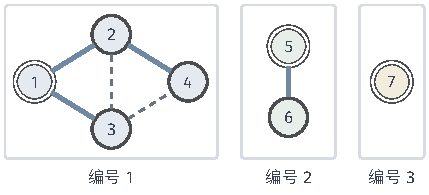
\includegraphics[width=72.592mm]{figures/01-basic-mathematics/04-graphs/tikz/c2-components-spanning-forest/figure.pdf}
  \caption{外层扫描与生成森林。图由贯穿四点图、边$\{5,6\}$和孤立点$7$组成，按编号扫描、每次启动广度优先遍历。三个分量分别获得编号$1,2,3$；双圈是每次遍历的起点，蓝色粗线是保留的父边，共$4=7-3$条，虚线边被检查过但未选入森林。}
  \label{fig:graph-trav-components-forest}
\end{figure}

生成森林可以用来检验输出：它应有$n-c$条边、不含环，并且同一棵树上的顶点标签相同。它只保留了谁和谁连通，不保留其他结构。

图~\ref{fig:graph-trav-components-forest}中第一个分量保留了$\{1,2\}$、$\{1,3\}$、$\{2,4\}$，舍弃了$\{2,3\}$和$\{3,4\}$。原图中$3$与$4$直接相邻，在森林中却要走$3\to1\to2\to4$三步；原图没有割点，而在森林中删去$1$或$2$都会把树断开。

边上若有权重，算法选出的边也没有任何总权最小的保证；在所有生成树中选总权最小的一棵，是第~\ref{sec:graph-minimum-spanning-tree}章的问题。

\subsection{增量无向图的连通分量}
\label{sec:graph-trav-union-find}

\subsubsection{问题与思路}

现在顶点集固定，边一条一条地加入，每加入一条边之后都可能被问到“两个给定顶点现在是否连通”。用上一小节的方法，每次加边后重新给全图打标签需要$O(n+m)$时间，加入$m$条边共要$O(m(n+m))$，太浪费。我们希望每次加边和每次查询都只花很少的时间。

加入边$\{u,v\}$对分量的影响很简单：若$u,v$原来已在同一分量，分量不变；否则把两个分量合并成一个。分量构成顶点集的一个划分，加边只会合并其中的两块，不会拆分。所以只需一种数据结构，维护若干互不相交的集合，支持两种操作：
\begin{itemize}
  \item $\operatorname{find}(v)$返回$v$所在集合的代表元，它扮演分量标签的角色，两顶点连通当且仅当代表元相同；
  \item $\operatorname{union}(u,v)$把$u$和$v$所在的两个集合合并。
\end{itemize}
这种数据结构称为\term{并查集}（union-find），也称不相交集合结构。

最直接的实现是让每个顶点直接存自己的标签。查询只需$O(1)$，但合并两个分量时，要把其中一个分量的所有顶点逐个改写标签，一次合并可能改写$O(n)$个顶点。改进的办法是不立即改写，而把每个集合组织成一棵有根树：合并时只改一个指针，查询时再顺着指针找到代表元。

\subsubsection{算法实现}

\paragraph{并查集的数据结构}
并查集维护两项状态：
\begin{itemize}
  \item 父指针$\operatorname{parent}(v)$：每个元素$v$在所属集合的树中的父元素；根的父指针指向自己，根就是集合的代表元；
  \item 集合大小$\operatorname{size}(r)$：只对根$r$有意义，记录这棵树中的元素个数。
\end{itemize}
初始时没有任何边，每个元素自成一个集合：$\operatorname{parent}(v)=v$，$\operatorname{size}(v)=1$。

图~\ref{fig:graph-trav-union-find-structure}画出了某一时刻的状态：两棵树对应两个集合，实际存储的只是右边两个长度为$n$的数组。$\operatorname{find}(4)$读$\operatorname{parent}(4)=3$，再读$\operatorname{parent}(3)=1$，到达指向自己的$1$，于是返回根$1$。合并两个集合只需把一个根的父指针改为另一个根，并更新新根的大小。

\begin{figure}[!htb]
  \centering
  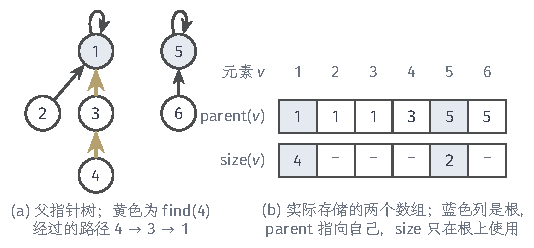
\includegraphics[width=82.952mm]{figures/01-basic-mathematics/04-graphs/tikz/c2-union-find-structure/figure.pdf}
  \caption{并查集的数据结构。元素$1,\ldots,6$分为集合$\{1,2,3,4\}$与$\{5,6\}$。(a)每个集合是一棵父指针树，箭头由元素指向父指针，根（蓝色）指向自己；$\operatorname{find}(4)$沿黄色路径$4\to3\to1$找到根。(b)计算机中实际存储的是$\operatorname{parent}$与$\operatorname{size}$两个数组，$\operatorname{size}$只在根上使用。}
  \label{fig:graph-trav-union-find-structure}
\end{figure}

合并时若随意选择谁接到谁下面，树可能退化成一条长链，查询要走很多步。下面的算法用两条规则避免这一点：合并时把小树接到大树下（按大小合并），查询时把经过的顶点直接接到根上（路径压缩）。

\begin{algorithm}[并查集的两种操作]
\label{alg:graph-trav-union-find}
状态：每个元素$v$的父指针$\operatorname{parent}(v)$，每个根$r$所在集合的大小$\operatorname{size}(r)$。初始时每个元素自成一个集合，$\operatorname{parent}(v)=v$，$\operatorname{size}(v)=1$。
\begin{enumerate}
  \item $\operatorname{find}(v)$：沿父指针从$v$走到根$r$；然后把这条路上经过的每个元素的父指针都直接改为$r$（路径压缩）；返回$r$。
  \item $\operatorname{union}(u,v)$：求$r_u=\operatorname{find}(u)$、$r_v=\operatorname{find}(v)$。若$r_u=r_v$，不做任何事。否则把较小集合的根接到较大集合的根下，大小相同时把$r_v$接到$r_u$下（按大小合并），并把新根的大小更新为两者之和。
\end{enumerate}
\end{algorithm}

\paragraph{增量连通分量的实现}
有了并查集，增量连通分量的维护就很直接。开始时顶点集上还没有边，为$V$中每个顶点建立一个单点集合，此时每个顶点自成一个分量。之后按到达次序处理两类请求：加入一条边$\{u,v\}$时调用一次$\operatorname{union}(u,v)$；询问$u,v$是否连通时，比较$\operatorname{find}(u)$与$\operatorname{find}(v)$是否相等。需要给每个顶点输出分量标签时，取$\operatorname{comp}(v)=\operatorname{find}(v)$即可。

这里的父指针只表示“属于同一集合”，与原图的边没有关系：合并$\{1,3\}$时，可能是$3$的根被接到$1$的根下，而原图中这两个根之间未必有边。需要输出原图中的连接时，应另外保存实际加入的边。

\paragraph{执行过程}
图~\ref{fig:graph-trav-union-find}按边序列$\{1,2\}$、$\{3,4\}$、$\{1,3\}$、$\{5,6\}$、$\{4,6\}$追踪这些操作，元素为$1,\ldots,6$。初始时六个元素各自为根。前两次合并各把一个单点接到另一个单点下：$\operatorname{parent}(2)=1$、$\operatorname{parent}(4)=3$，得到$\{1,2\}$与$\{3,4\}$，此时还有单点集合$\{5\}$、$\{6\}$。

合并$\{1,3\}$时两个集合大小都是$2$，按约定把根$3$接到根$1$下，$\operatorname{size}(1)=4$，$4$的深度变为$2$。之后若查询$\operatorname{find}(4)$，沿$4\to3\to1$找到根$1$，路径压缩把$4$的父指针直接改为$1$，下次查询只需一步。

合并$\{5,6\}$得到大小为$2$的集合；处理$\{4,6\}$时，$4$所在集合大小为$4$、$6$所在集合大小为$2$，于是根$5$接到根$1$下，全部六个元素属于同一集合。每一步后的集合划分都与“已加入的边构成的图的连通分量”一致。

\begin{figure}[!htb]
  \centering
  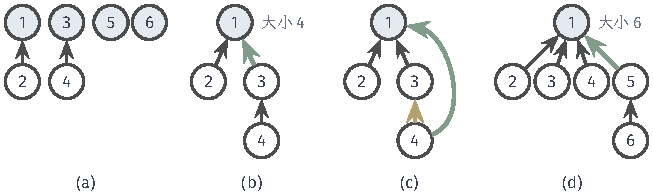
\includegraphics[width=110.500mm]{figures/01-basic-mathematics/04-graphs/tikz/c2-union-find/figure.pdf}
  \caption{并查集的父指针树，箭头由元素指向其父指针，蓝色填充为根。(a)合并$\{1,2\}$、$\{3,4\}$后；(b)合并两个大小为$2$的集合，按约定把根$3$接到根$1$下（绿色箭头）；(c)查询$\operatorname{find}(4)$经过$4\to3\to1$（黄色虚线是原父指针），路径压缩后$4$直接指向根$1$；(d)合并$\{5,6\}$后再处理$\{4,6\}$，较小集合的根$5$接到较大集合的根$1$下。}
  \label{fig:graph-trav-union-find}
\end{figure}

\subsubsection{算法分析}

\paragraph{正确性}
并查集的正确性来自一个保持不变的性质：在任何时刻，并查集中的集合恰好是已加入的边构成的图的连通分量。初始时没有边，每个顶点自成分量，集合也都是单点。加入边$\{u,v\}$时，若$u,v$已在同一集合，分量不变，算法也不做任何事；否则两个分量合并，算法恰好把对应的两个集合合并。路径压缩只改变树的形状，不改变哪些元素在同一棵树中。

\paragraph{复杂度}
查询的代价取决于树高，而按大小合并保证树不会太高。

\begin{theorem}[按大小合并的树高]
\label{thm:graph-trav-union-by-size}
只使用按大小合并（无论是否路径压缩）时，任一元素到根的路径长度不超过$\log_2 n$，其中$n$是元素总数。
\end{theorem}

\begin{proof}
先不考虑路径压缩。一个元素的深度只在它所在的根被接到另一个根下面时增加$1$；按规则，被接的那一侧不大于另一侧，所以合并后该元素所在集合的大小至少是原来的两倍。集合大小从$1$开始，不超过$n$，至多翻倍$\log_2 n$次，深度也就至多为$\log_2 n$。路径压缩只把元素的父指针改为它的某个祖先，只会让深度变小，不影响这个上界。
\end{proof}

由定理~\ref{thm:graph-trav-union-by-size}，每次$\operatorname{find}$和$\operatorname{union}$都只需$O(\log n)$时间，存储为$O(n)$。

路径压缩使反复查询同一区域变得更快。可以证明，两条规则同时使用时，任意$k$次操作的总时间为$O(k\,\alpha(n))$，其中$\alpha$是增长极慢的反Ackermann函数，对任何实际规模的$n$都不超过$4$；这一摊还分析较长，这里不展开，使用时只需记住每次操作的平均代价几乎是常数。与每次加边后重新遍历的$O(n+m)$相比，差距随图的规模迅速拉大。

\paragraph{适用范围}
并查集适合“只加边、不删边”的情形。第~\ref{sec:graph-minimum-spanning-tree}章的Kruskal算法按边权从小到大考虑每条边，需要判断加入这条边是否会成环，也就是判断两个端点是否已在同一分量，正好用并查集完成。删除一条边可能把一个分量拆成两个，而并查集的合并无法撤销，所以它不能直接维护任意删边后的分量。在图像中给相连的像素区域编号时，也常先给像素临时标号、再用并查集合并相遇的标号，具体扫描方式不在本卷讨论。

\subsection{有向图的强连通分量}
\label{sec:graph-trav-scc}

\subsubsection{问题与思路}

输入是有向图$\mathcal G=(V,E)$的出邻接表，要给每个顶点打上强分量标签$\operatorname{comp}(v)$，使得$\operatorname{comp}(u)=\operatorname{comp}(v)$当且仅当$u$与$v$相互可达。照搬无向图的做法，从$r$出发遍历一次，找到的是$r$能到达的全部顶点，而强分量要求双向可达。图~\ref{fig:graph-trav-scc-reach}(a)中，从$1$出发能到达$1,2,3,4$，但$3,4$回不到$1$，$1$所在的强分量只是$\{1,2\}$。

第~\ref{sec:graph-conn-strong-weak}小节已经说明，$v$所在的强分量等于“从$v$可达的顶点”与“能到达$v$的顶点”的交集，图~\ref{fig:graph-trav-scc-reach}在本例上画出了这两个集合。后者可以在把所有弧反向后的图上从$v$遍历得到。但对每个顶点都这样做两次遍历，需要$O(n(n+m))$时间。

\begin{figure*}[!htb]
  \centering
  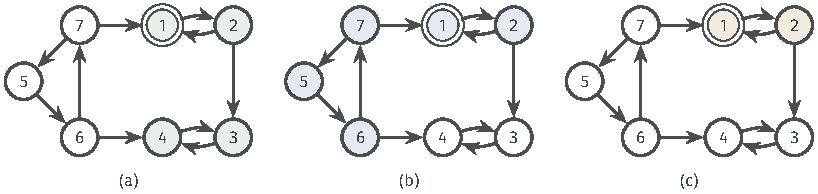
\includegraphics[width=138.400mm]{figures/01-basic-mathematics/04-graphs/tikz/c2-scc-forward-backward/figure.pdf}
  \caption{强连通分量是前向可达集与后向可达集的交。图中弧为$1\to2$、$2\to1$、$2\to3$、$3\to4$、$4\to3$、$5\to6$、$6\to4$、$6\to7$、$7\to1$、$7\to5$，双圈为顶点$1$。(a)从$1$出发可达$\{1,2,3,4\}$；(b)能到达$1$的顶点为$\{1,2,5,6,7\}$；(c)两者的交$\{1,2\}$就是$1$所在的强连通分量。}
  \label{fig:graph-trav-scc-reach}
\end{figure*}

更快的办法只需两遍遍历，关键是在反向图上选对起点。把有向图$\mathcal G$的每条弧$u\to v$改为$v\to u$，得到\term{反向图}（reverse graph）$\mathcal G^{\mathrm{rev}}$。$\mathcal G$与$\mathcal G^{\mathrm{rev}}$的强连通分量相同，因为相互可达的两个顶点在弧全部反向后仍然相互可达。在反向图上从$v$遍历，找到的是原图中能到达$v$的顶点，它包含$v$的强分量，也可能越出去。越出去的部分都是原图中位于$v$的分量“上游”的分量。

关键在于起点的顺序。如果每次都从一个“没有未处理的上游分量”的分量中选起点，在反向图上的遍历就只能走到已经处理过的分量或者本分量内部；只要已处理的顶点不再进入，这次遍历就恰好停在本分量的边界上。这个顺序由第一遍深度优先遍历的完成时刻提供：完成时刻最大的顶点，位于最上游的分量中。这一方法称为\term{Kosaraju算法}（Kosaraju's algorithm）。

\subsubsection{算法实现}

算法开始前，先扫描一遍出邻接表，构造反向图$\mathcal G^{\mathrm{rev}}$的邻接表，也就是原图的入邻接表。它只是第二遍要读取的输入，在算法运行中不再改变。

此后分两遍进行，各自维护的状态是：
\begin{itemize}
  \item 第一遍：深度优先遍历的全部状态（第~\ref{sec:graph-trav-dfs-stack}小节），另加一张完成次序表，按完成的先后记下顶点；
  \item 第二遍：标签数组$\operatorname{comp}(\cdot)$，初始全为$0$；已用的标签个数$c$，初始为$0$。
\end{itemize}
第一遍在原图上做完整的深度优先遍历，填好完成次序表。第二遍按完成时刻从大到小扫描顶点，遇到未标记的顶点$r$，令$c\gets c+1$，在反向图上从$r$遍历，只进入未标记的顶点，把到达的顶点标为$c$。

\begin{algorithm}[Kosaraju强连通分量算法]
\label{alg:graph-trav-kosaraju}
输入：有向图$\mathcal G=(V,E)$的出邻接表。输出：每个顶点所属强连通分量的编号。
\begin{enumerate}
  \item 扫描出邻接表，构造反向图$\mathcal G^{\mathrm{rev}}$的出邻接表，即原图的入邻接表。
  \item 在$\mathcal G$上执行完整的深度优先遍历（算法~\ref{alg:graph-trav-dfs}），覆盖全部顶点，记录完成次序。
  \item 所有顶点置为未标记。按完成时刻从大到小扫描顶点；遇到未标记的顶点$r$时，开始一个新分量，在$\mathcal G^{\mathrm{rev}}$上从$r$遍历（广度或深度优先均可），只进入未标记的顶点，把这次到达的顶点全部标为这个分量。
\end{enumerate}
\end{algorithm}

\paragraph{执行过程}
仍用图~\ref{fig:graph-trav-scc-reach}中的有向图。它的强连通分量是$\{5,6,7\}$、$\{1,2\}$和$\{3,4\}$，分量之间只有单向的弧。

第一遍按编号选择起点、按编号读取出邻居，共启动两次：
\begin{itemize}
  \item 从$1$出发，依次发现$1,2,3,4$；$4$的出邻居$3$在栈中，$4$完成，随后$3,2,1$依次完成，完成时刻为$f(4)=5$、$f(3)=6$、$f(2)=7$、$f(1)=8$。
  \item 从$5$重新出发，发现$5,6$；$6$的出邻居$4$已完成，跳过，再发现$7$；$7$的出邻居$1$已完成、$5$在栈中，于是$7,6,5$依次完成，$f(7)=12$、$f(6)=13$、$f(5)=14$。
\end{itemize}
完成次序为$4,3,2,1,7,6,5$，见图~\ref{fig:graph-trav-kosaraju}(a)。

第二遍按完成时刻从大到小，即$5,6,7,1,2,3,4$选择起点，在反向图上遍历，见图~\ref{fig:graph-trav-kosaraju}(b)。三次遍历依次为：
\begin{itemize}
  \item 从$5$出发，令$c=1$，反向弧把它引向$7$，再引向$6$；$\{5,6,7\}$中没有反向弧通往别处，于是$\operatorname{comp}(5)=\operatorname{comp}(6)=\operatorname{comp}(7)=1$。扫描到$6,7$时已标记，跳过。
  \item 下一个未标记的是$1$，令$c=2$：反向弧$1\to2$、$1\to7$中$7$已标记，只进入$2$，得到$\{1,2\}$。
  \item 最后从$3$出发，令$c=3$，反向弧$3\to2$通往已标记的$2$，只进入$4$，得到$\{3,4\}$。
\end{itemize}
每次遍历恰好停在一个强分量的边界上。

\begin{figure*}[!htb]
  \centering
  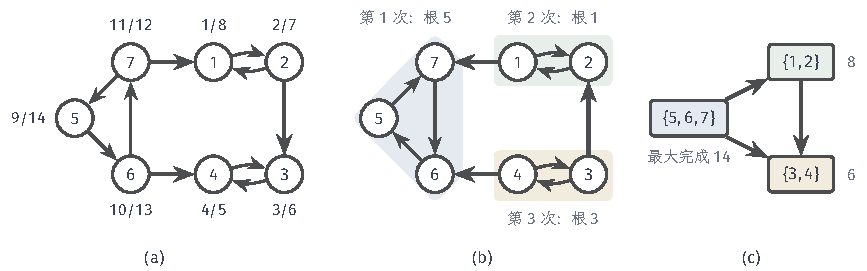
\includegraphics[width=146.500mm]{figures/01-basic-mathematics/04-graphs/tikz/c2-kosaraju-condensation/figure.pdf}
  \caption{Kosaraju算法的两遍过程与缩点图。(a)原图上按编号重启的深度优先遍历，顶点旁为发现/完成时刻；粗箭头是连接不同强分量的弧。(b)反向图上按完成时刻从大到小（$5,6,7,1,2,3,4$）选择起点，三次遍历分别得到蓝、绿、黄三个强连通分量，指向已标记分量的反向弧不再进入。(c)把每个强分量缩成一点得到的缩点图，旁注为各分量中最大的完成时刻；缩点图无环，且最大完成时刻沿弧方向递减。}
  \label{fig:graph-trav-kosaraju}
\end{figure*}

\subsubsection{算法分析}

\paragraph{正确性}
第二遍之所以不会越界，是因为第一遍的完成时刻在分量之间有固定的先后。对强连通分量$C$，记其中最大的完成时刻为
\[
f(C)=\max_{v\in C}f(v).
\]
在上例中，$f(\{5,6,7\})=14$、$f(\{1,2\})=8$、$f(\{3,4\})=6$，而分量之间的弧都从$f$值大的指向$f$值小的，即从上游指向下游。

\begin{lemma}[分量间的完成时刻]
\label{lem:graph-trav-scc-finish}
设$C\neq C'$是有向图的两个强连通分量，且存在一条从$C$中顶点指向$C'$中顶点的弧。则在一次完整的深度优先遍历中，$f(C)>f(C')$。
\end{lemma}

\begin{proof}
考察$C\cup C'$中最先被发现的顶点$x$。

若$x\in C$。在时刻$d(x)$，$C\cup C'$中其余顶点都未发现。$C$中每个顶点都能从$x$经$C$内部的路径到达；$C'$中每个顶点都能先在$C$内走到那条弧的起点，经弧进入$C'$，再在$C'$内部到达。这些路径上的顶点此时都未发现，由引理~\ref{lem:graph-trav-white-path}，$C\cup C'$中其余顶点都成为$x$的后代并先于$x$完成，所以$f(C)=f(x)>f(C')$。

若$x\in C'$。同理，$C'$中其余顶点都成为$x$的后代，$f(C')=f(x)$。另一方面，从$C'$中的任何顶点都不能到达$C$：否则结合已有的从$C$到$C'$的弧，$C$与$C'$中的顶点相互可达，它们就应属于同一个强分量。所以在$x$处于处理中期间，$C$中没有顶点被发现（那样的顶点会是$x$的后代，从而从$x$可达）。$C$中顶点都在$f(x)$之后才被发现，也就在$f(x)$之后完成，所以$f(C)>f(x)=f(C')$。
\end{proof}

在反向图中，这个不等式的方向随弧一起反转：从分量$C$出发的反向弧只能通往$f$值更大的分量。第二遍按$f$值从大到小选择起点，这些分量在轮到$C$之前都已标记，于是遍历被挡在$C$之内。

\begin{theorem}[Kosaraju算法的正确性]
\label{thm:graph-trav-kosaraju}
算法~\ref{alg:graph-trav-kosaraju}第三步的每一次遍历，恰好标记一个强连通分量的全部顶点。
\end{theorem}

\begin{proof}
对第二遍已经完成的遍历次数归纳，假设此前每次遍历都恰好标记了一个完整的强分量。设下一个起点是$r$，所在分量为$C$。$r$是未标记顶点中完成时刻最大的；由归纳假设，未标记的顶点恰好组成若干个完整的强分量，所以$f(r)=f(C)$，且$C$在未标记的分量中$f$值最大。

$C$在反向图中仍然强连通，从$r$出发能到达$C$的全部顶点，而$C$中的顶点都未标记，因此都会被这次遍历标记。另一方面，设反向图中有一条弧从$C$中顶点指向另一个分量$C'$中的顶点，它对应原图中一条从$C'$指向$C$的弧，由引理~\ref{lem:graph-trav-scc-finish}有$f(C')>f(C)$。而$C$是未标记分量中$f$值最大的，所以$C'$已经被标记，这次遍历不会进入。因此这次遍历标记的恰好是$C$。
\end{proof}

这一论证依赖算法的三处细节，缺一不可：
\begin{itemize}
  \item 第一遍必须覆盖全部顶点，否则有些顶点没有完成时刻；
  \item 第二遍必须在反向图上进行，若在原图上从$5$遍历，会经$6\to4$、$7\to1$走进另外两个分量；
  \item 起点必须按完成时刻从大到小选择，若改为从小到大，上例中第二遍会先从$4$出发，在反向图上经$4\to6$进入$\{5,6,7\}$，再经$3\to2$进入$\{1,2\}$，把三个分量全部混在一起。
\end{itemize}

\paragraph{复杂度}
第一遍深度优先遍历用$O(n+m)$时间。构造反向图需要扫描每条弧一次，时间与额外存储都是$O(n+m)$。第二遍按完成时刻从大到小扫描，只需把第一遍的完成次序倒过来读，不必排序；遍历本身再用$O(n+m)$时间。总时间为$O(n+m)$，与无向图的分量编号同阶，远小于逐点求两个可达集的$O(n(n+m))$。

\subsubsection{缩点图}
\label{sec:graph-trav-condensation}

得到强连通分量后，可以把每个分量当作一个整体，压缩为一个顶点。若原图中有从分量$C$指向另一分量$C'$的弧，就在$C$与$C'$之间连一条弧$C\to C'$（多条这样的弧只保留一条，分量内部的弧舍去），得到的有向图称为\term{缩点图}（condensation graph）。图~\ref{fig:graph-trav-kosaraju}(c)中，缩点图有三个顶点和三条弧$\{5,6,7\}\to\{1,2\}$、$\{1,2\}\to\{3,4\}$、$\{5,6,7\}\to\{3,4\}$。

\begin{theorem}[缩点图无环]
\label{thm:graph-trav-condensation-dag}
任何有限有向图的缩点图都是有向无环图。
\end{theorem}

\begin{proof}
假设缩点图中有有向环$C_1\to C_2\to\cdots\to C_k\to C_1$，$k\geq2$，各$C_i$是不同的强分量。每条弧$C_i\to C_{i+1}$对应原图中一条从$C_i$中某顶点到$C_{i+1}$中某顶点的弧，而每个分量内部任意两点相互可达。于是从$C_1$中任一顶点出发，可以依次经过$C_2,\ldots,C_k$再回到$C_1$，环上所有分量中的顶点两两相互可达，它们应属于同一个强分量，与$C_1,\ldots,C_k$互不相同矛盾。
\end{proof}

由引理~\ref{lem:graph-trav-scc-finish}，缩点图中每条弧都从$f$值较大的分量指向$f$值较小的分量，所以Kosaraju算法第二遍得到分量的先后次序，恰好使缩点图的每条弧从先得到的分量指向后得到的分量。上例中得到的次序$\{5,6,7\}$、$\{1,2\}$、$\{3,4\}$就满足这一点。任何有向图都可以先缩点、再在无环的缩点图上安排先后，这正是下一节要研究的依赖排序。

\section{拓扑排序}
\label{sec:graph-topological-order}

一组任务中，有的任务要等另一些任务完成才能开始；计算一组中间量时，一个量要等它依赖的量算出来才能计算。用有向图表示这类依赖，弧$u\to v$表示$u$必须先于$v$处理，问题就是给所有顶点排出一个满足全部依赖的次序。

这样的次序只在无环图上存在；构造它有两种方法，Kahn算法逐个取出没有依赖的顶点，基于深度优先遍历的方法反转完成次序。两种方法遇到有向环时都报告失败，而不是输出一个不完整的序列。

\subsection{问题与存在条件}
\label{sec:graph-trav-topo-problem}

把依赖次序写成顶点的排列，要求就是每条弧的起点排在终点之前。

\begin{definition}[拓扑序]
\label{def:graph-trav-topological-order}
有向图$\mathcal G=(V,E)$的\term{拓扑序}（topological order）是$V$中全部顶点的一个排列$v_1,v_2,\ldots,v_n$，使得对每条弧$v_i\to v_j$都有$i<j$。求拓扑序的过程称为拓扑排序。
\end{definition}

拓扑序只要求每条弧前后正确，没有弧相连的两个顶点谁先谁后都可以，因此拓扑序一般不唯一。检验一个输出是否正确，标准是逐条弧核对先后，而不是与某一个特定答案比较。

并非每个有向图都有拓扑序。若图中有有向环$v_1\to v_2\to\cdots\to v_k\to v_1$，排列既要让$v_1$在$v_2$之前、$v_2$在$v_3$之前……$v_{k-1}$在$v_k$之前，又要让$v_k$在$v_1$之前，这不可能。所以有拓扑序的图一定没有有向环。

反过来，无环时可以先排没有依赖的顶点。排在第一位的顶点不能有任何前驱，也就是入度为$0$。把它排好后，它对后继的约束就都满足了，可以把它和它的出弧从图中删去，在剩下的图上重复同样的事。这个想法能否一直进行下去，取决于每一步是否总能找到入度为$0$的顶点。

\begin{lemma}[有向无环图有源点]
\label{lem:graph-trav-dag-source}
非空的有限有向无环图至少有一个入度为$0$的顶点。
\end{lemma}

\begin{proof}
假设每个顶点的入度都至少为$1$。从任一顶点$v_0$出发，取它的一个前驱$v_1$，即有弧$v_1\to v_0$；再取$v_1$的一个前驱$v_2$，如此继续。顶点只有有限个，这个序列中必有某个顶点第二次出现，设$v_i=v_j$，$i<j$。则$v_j\to v_{j-1}\to\cdots\to v_i$是一个有向环，与无环矛盾。
\end{proof}

\begin{theorem}[拓扑序的存在性]
\label{thm:graph-trav-topological-existence}
有限有向图存在拓扑序，当且仅当它是有向无环图。
\end{theorem}

\begin{proof}
必要性已在上面说明。充分性对顶点数$n$归纳。$n=0$时空排列即为拓扑序。设$n\geq1$，由引理~\ref{lem:graph-trav-dag-source}取一个入度为$0$的顶点$v_1$。删去$v_1$及其出弧，剩下的是原图的诱导子图，删去顶点不会产生新的环，它仍是有向无环图，由归纳假设有拓扑序$v_2,\ldots,v_n$。在前面补上$v_1$：以$v_1$为起点的弧终点都在后面；$v_1$没有入弧；其余弧都在剩下的图中，已经满足要求。所以$v_1,v_2,\ldots,v_n$是原图的拓扑序。
\end{proof}

这个证明本身就是一个构造：不断取出入度为$0$的顶点。

\subsection{Kahn算法}
\label{sec:graph-trav-kahn}

照上一小节的构造真的从图中删去顶点，代价很大，而且每一步还要重新寻找入度为$0$的顶点。实际上只需维护每个顶点在“尚未输出的顶点构成的子图”中的当前入度：输出一个顶点$u$时，它的每条出弧$u\to v$不再计入，把$v$的当前入度减一。哪个顶点的当前入度刚降到$0$，它就可以输出了，把它放进一个等待队列。这一方法称为\term{Kahn算法}（Kahn's algorithm）。

算法维护三项状态：
\begin{itemize}
  \item 每个顶点的当前入度$\operatorname{indeg}(v)$；
  \item 一个队列$Q$，存放当前入度为$0$、尚未输出的顶点；
  \item 输出序列$L$。
\end{itemize}
初始化时扫描全部弧统计入度，把所有入度为$0$的顶点（包括孤立点）放入$Q$，$L$为空。此后每一轮从$Q$取出一个顶点$u$，追加到$L$的末尾，再检查$u$的每条出弧$u\to v$，令$\operatorname{indeg}(v)\gets\operatorname{indeg}(v)-1$，若它恰好降为$0$，把$v$放入$Q$。$Q$为空时停止。

\begin{algorithm}[Kahn拓扑排序]
\label{alg:graph-trav-kahn}
输入：有向图$\mathcal G=(V,E)$的出邻接表。输出：一个拓扑序，或报告图中有有向环。
\begin{enumerate}
  \item 扫描全部弧，统计每个顶点的入度$\operatorname{indeg}(v)$。把所有入度为$0$的顶点（包括孤立点）放入队列$Q$，输出序列$L$置空。
  \item 当$Q$非空时，取出队首$u$，追加到$L$末尾。对每条出弧$u\to v$，令$\operatorname{indeg}(v)\gets\operatorname{indeg}(v)-1$；若它恰好降为$0$，把$v$放入$Q$。
  \item $Q$为空时停止。若$L$含全部$n$个顶点，输出$L$；否则报告有有向环。
\end{enumerate}
\end{algorithm}

一个顶点只在当前入度刚降到$0$的那一刻入队，因此不会重复入队。判断必须用当前入度，而不是初始入度：初始入度为$1$的顶点，在它唯一的前驱输出之前不能输出。

\paragraph{执行过程}
考虑弧为$1\to2$、$1\to3$、$2\to4$、$3\to4$的菱形依赖：任务$2,3$都依赖$1$，任务$4$同时依赖$2$和$3$。初始入度为$(0,1,1,2)$，只有$1$入队，$Q=[1]$。图~\ref{fig:graph-trav-kahn}(b)列出了每次输出后的变化：
\begin{itemize}
  \item 输出$1$后，$2,3$的入度都降为$0$，两者入队，$Q=[2,3]$；
  \item 输出$2$后，$4$的入度从$2$降为$1$，还不能入队，$Q=[3]$；
  \item 输出$3$后，$4$的入度降为$0$，入队，$Q=[4]$；
  \item 最后输出$4$，$Q$为空。
\end{itemize}
$L=1,2,3,4$含全部顶点，是一个拓扑序。

\begin{figure}[!htb]
  \centering
  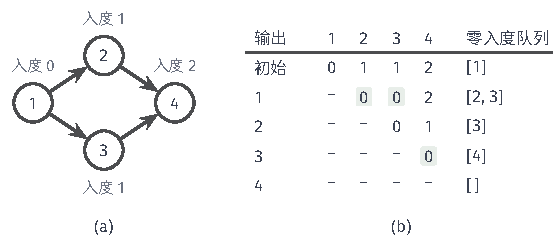
\includegraphics[width=94.8mm]{figures/01-basic-mathematics/04-graphs/tikz/c2-kahn-diamond/figure.pdf}
  \caption{Kahn算法在菱形依赖图上的执行。(a)依赖图及各顶点的初始入度。(b)每输出一个顶点后各顶点的当前入度（“--”表示已输出）与零入度队列；绿色底纹标出刚降为$0$、随即入队的入度。顶点$4$要等两个前驱都输出后才入队。}
  \label{fig:graph-trav-kahn}
\end{figure}

输出$1$之后，$2$和$3$同时位于队列中，这表示两项任务可以同时执行，或以任意先后执行。若先取$3$，就得到同样合法的$1,3,2,4$。队列中同时有多个零入度顶点时选哪一个，决定了得到哪个拓扑序。

\paragraph{正确性}
先看无环的情形。尚未输出的顶点构成原图的诱导子图，仍是有向无环图；只要它非空，由引理~\ref{lem:graph-trav-dag-source}就有当前入度为$0$的顶点，而这样的顶点在入度降为$0$时已经入队。因此队列在全部顶点输出之前不会变空，$L$最终含全部$n$个顶点。对每条弧$u\to v$，$v$的当前入度要等$u$输出后才扣除这条弧的贡献，所以$v$只能在$u$之后入队、之后输出，$L$满足拓扑序的要求。

再看有环的情形。环上每个顶点在环上都有一个前驱，环上第一个被输出的顶点在输出之前当前入度至少为$1$，不可能入队，所以环上的顶点一个也不会输出，$L$少于$n$个顶点，算法报告有环。这时已经输出的部分只是一个前缀，不能当作完整的拓扑序。若需要给出环本身，可以在剩下的顶点中重复引理~\ref{lem:graph-trav-dag-source}证明中的“不断取前驱”，必然在有限步内回到已经走过的顶点，找到一个有向环。

\paragraph{复杂度}
统计入度要扫描每条弧一次；之后每个顶点入队、出队各一次，每条弧在其起点输出时被扣减一次。总时间为$O(n+m)$，入度数组、队列与输出序列占$O(n)$额外空间。

若要求结果可复现，例如在多个零入度顶点中总是选编号最小的，就要把普通队列换成优先队列，每次入队、出队需要$O(\log n)$时间，总时间变为$O(m+n\log n)$。

\subsection{基于DFS的拓扑排序}
\label{sec:graph-trav-dfs-toposort}

第~\ref{sec:graph-trav-dfs-orders}小节看到，深度优先遍历中一个顶点的后代都先于它完成。在依赖图中，从$u$出发能走到的顶点都排在$u$之后；若它们都比$u$先完成，那么把完成次序反转，$u$就排在它们前面。所以做一次深度优先遍历，按完成时刻从大到小输出顶点即可。被$u$的弧指向、却不是$u$后代的顶点同样先于$u$完成，这由后面的定理保证。

算法的状态就是深度优先遍历的状态（三种状态、栈、时钟），再加一个初始为空的输出序列$L$。遍历按算法~\ref{alg:graph-trav-dfs}进行，更新规则只增加两处：
\begin{itemize}
  \item 每当一个顶点完成时，把它放到$L$的最前面，遍历结束时$L$就已是逆完成次序；
  \item 每当读到的出邻居处于处理中，即遇到回边，就沿父指针取出一个有向环并停止，拒绝输出排序。
\end{itemize}
若整次遍历没有遇到回边，输出$L$。

\paragraph{执行过程}
在同一个菱形依赖图上，从$1$出发、按编号读取出邻居，$L$的变化依次为：
\begin{itemize}
  \item 发现$1,2,4$；$4$没有出邻居，完成，$L=[4]$；
  \item 回到$2$，$2$完成，$L=[2,4]$；
  \item 回到$1$后发现$3$，$3$的出邻居$4$已完成，不进入，$3$完成，$L=[3,2,4]$；
  \item 最后$1$完成，$L=[1,3,2,4]$。
\end{itemize}
完成次序为$4,2,3,1$，$L$正是它的反转。它与Kahn算法给出的$1,2,3,4$不同，但两者都是合法拓扑序：如图~\ref{fig:graph-trav-dfs-toposort}(b)，把顶点按次序从左到右排开，四条弧全部指向右方。

\begin{figure}[!htb]
  \centering
  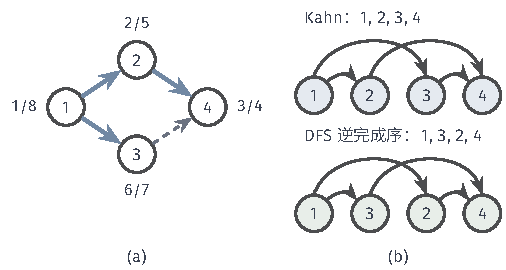
\includegraphics[width=93.8mm]{figures/01-basic-mathematics/04-graphs/tikz/c2-dfs-topological-order/figure.pdf}
  \caption{基于深度优先遍历的拓扑排序。(a)菱形依赖图上从$1$出发的深度优先遍历，旁注为发现/完成时刻，蓝色箭头为父指针对应的弧，虚线弧$3\to4$检查时$4$已完成。(b)Kahn算法得到的$1,2,3,4$与逆完成次序$1,3,2,4$，两种排列下每条弧都从左指向右，都是合法拓扑序。}
  \label{fig:graph-trav-dfs-toposort}
\end{figure}

\paragraph{正确性}
有环时，由定理~\ref{thm:graph-trav-directed-cycle}，遍历一定会遇到回边，算法报告环而不输出排序。无环时，下面的定理说明逆完成次序总是拓扑序。

\begin{theorem}[逆完成次序是拓扑序]
\label{thm:graph-trav-dfs-toposort}
对有向无环图执行一次覆盖全部顶点的深度优先遍历，则对每条弧$u\to v$都有$f(v)<f(u)$。因此按完成时刻从大到小排列顶点，得到一个拓扑序。
\end{theorem}

\begin{proof}
考察$u$检查弧$u\to v$的时刻，此时$u$处于处理中，按$v$的状态分三种情况。若$v$未发现，它将以$u$为父指针被发现，由引理~\ref{lem:graph-trav-dfs-nesting}，$f(v)<f(u)$。若$v$已完成，$f(v)$早于当前时刻，而$u$尚未完成，同样$f(v)<f(u)$。若$v$处于处理中，$u\to v$是一条回边，由定理~\ref{thm:graph-trav-directed-cycle}图中有有向环，与假设矛盾，这种情况不会发生。
\end{proof}

定理要求遍历覆盖全部顶点。只从一个起点遍历时，得到的只是它可达部分的完成次序。在菱形图中若只从$2$出发，只能到达$2,4$，反转后是$2,4$，漏掉了$1$和$3$。

也不能把各次重启的结果分别反转后简单拼接：先从$2$出发得到$2,4$，再从$1$出发得到$1,3$，拼成$2,4,1,3$，违反了弧$1\to2$。正确做法是把整次遍历的完成次序$4,2,3,1$作为一个整体反转，得到$1,3,2,4$；定理~\ref{thm:graph-trav-dfs-toposort}的证明对跨越不同起点的弧同样成立。按上面“完成时放到最前面”的实现，各次重启共用同一个$L$，自然就是整体反转。

把完成的顶点放到$L$最前面，每次只需常数时间（例如用链表，或先追加到末尾、最后整体反转一次），所以总时间就是一次深度优先遍历的$O(n+m)$，额外空间为$O(n)$。

\subsection{两种方法的比较}
\label{sec:graph-trav-topo-comparison}

两种方法的时间都是$O(n+m)$，在无环图上都输出合法的拓扑序，在有环图上都报告失败，但维护的信息不同。Kahn算法显式地维护“当前可以执行的任务”这一集合，即零入度队列，适合需要逐步列出可并行任务、或按某种优先规则选择任务的场合。基于深度优先遍历的方法不需要入度数组，在已经要做深度优先遍历、或需要在有环时直接给出环的场合可以复用同一次遍历。

对含环的一般有向图，可以先用第~\ref{sec:graph-trav-scc}小节的方法求出强连通分量并缩点，再对无环的缩点图做拓扑排序，这样得到的是分量之间的先后。第~\ref{chap:shortest-paths}章在有向无环图上计算最短路时，就是按拓扑序逐个处理顶点：处理到一个顶点时，它的所有前驱都已处理完毕。

\section{基于分隔集的分块}
\label{sec:graph-separator-blocks}

大图上的计算常常希望“分而治之”：把图拆成几块分别处理，再在块与块的连接处汇总。第~\ref{sec:graph-connectivity-separation}节定义了分隔集：删除一个顶点集$S$后，若某些顶点之间不再有路径，$S$就把它们分隔开。

本节接受一个给定的候选集$S$，检验它是否真的把图拆成了几侧，并把图分成共享接口的局部块。分块只依据结构，不涉及怎样寻找好的分隔集；块上的数值怎样沿接口组合，在第~\ref{part:graph-dynamic-programming}部分讨论。

\subsection{问题与思路}
\label{sec:graph-trav-delete-separator}

输入是无向图$\mathcal G=(V,E)$和一个候选集合$S\subseteq V$。要回答两件事：删除$S$之后，其余顶点分成了几侧，每侧是哪些顶点；以及怎样把原图分成若干块，使每块对应一侧，块与块之间只通过$S$联系，并且原图的每条边都保存在某个块中。是否拆分成功只能由计算结果判断，不能因为输入被称作“分隔集”就默认成立。

办法是先删去$S$求分量，再把$S$加回。删除$S$中的顶点及与它们关联的边，得到$\mathcal G-S$，即$V\setminus S$上的诱导子图。它的连通分量$C_1,\ldots,C_r$就是“各侧”：不同的$C_j$之间在$\mathcal G-S$中没有边，所以原图中从$C_j$到$C_k$（$j\neq k$）的任何路径都必须经过$S$。按$r$的取值有三种结果：
\begin{itemize}
  \item $r\geq2$时，$S$把图拆成了$r$侧；
  \item $r=1$时，删除$S$后其余顶点仍然连通，$S$没有形成多侧拆分；
  \item $r=0$时$S=V$，余图为空，也谈不上拆分。
\end{itemize}

删除$S$的同时，各分量与$S$之间的边、$S$内部的边也丢失了。要把原图完整地分成几块，还要把$S$加回每一侧，得到\term{局部块}（local block）
\begin{equation}
\mathcal B_j=\mathcal G[C_j\cup S],\qquad j=1,\ldots,r,
\label{eq:graph-trav-local-block}
\end{equation}
其中$S$称为各块的公共接口。求各侧正是第~\ref{sec:graph-trav-components-forest}小节的连通分量问题，只是要把$S$中的顶点当作不存在。

\subsection{算法实现}
\label{sec:graph-trav-separator-implementation}

实现时不必真的从邻接表中删去$S$。算法开始前，用一个布尔数组把$S$中的顶点标记为“屏蔽”；这个数组只是对输入的标注，运行中不再改变。此后的计算就是在未屏蔽的顶点上做第~\ref{sec:graph-trav-components-forest}小节的分量编号，维护的状态是：
\begin{itemize}
  \item 标签数组$\operatorname{comp}(\cdot)$：未屏蔽顶点所属的分量编号，$0$表示尚未标记，初始全为$0$；
  \item 分量个数$r$：初始为$0$；
  \item 所用遍历的队列或栈，初始为空。
\end{itemize}
更新规则与算法~\ref{alg:graph-trav-components}相同，只多了两处跳过：
\begin{itemize}
  \item 外层扫描：遇到屏蔽顶点或已标记的顶点跳过；遇到未屏蔽且未标记的顶点$v$，令$r\gets r+1$，置$\operatorname{comp}(v)=r$，从$v$启动遍历。
  \item 遍历：读到邻居$w$时，若$w$被屏蔽或已标记就不进入；否则置$\operatorname{comp}(w)=r$，把$w$放入队列或栈。
\end{itemize}
扫描结束后，标签为$j$的顶点组成$C_j$。再按$r$报告结果，并为每个分量列出局部块的顶点$C_j\cup S$。

\begin{algorithm}[删除候选集后的分量与局部块]
\label{alg:graph-trav-separator-components}
输入：无向图的邻接表，候选集合$S\subseteq V$。输出：$\mathcal G-S$的连通分量$C_1,\ldots,C_r$，拆分是否成功（$r\geq2$），以及局部块$\mathcal B_1,\ldots,\mathcal B_r$。
\begin{enumerate}
  \item 用一个布尔数组标记$S$中的顶点为“屏蔽”，不修改原邻接表。
  \item 对未屏蔽的顶点执行算法~\ref{alg:graph-trav-components}：外层扫描跳过屏蔽顶点，遍历时读到屏蔽的邻居一律跳过。
  \item 输出各分量；若$r\geq2$报告拆分成功，$r=1$报告未拆分，$r=0$报告余图为空。
  \item 对每个$j$，以$C_j\cup S$为顶点集输出局部块$\mathcal B_j$；其中$S$的顶点和$S$内部的边只记录对原图的引用。
\end{enumerate}
\end{algorithm}

\paragraph{执行过程}
在贯穿四点图上取$S=\{2,3\}$。屏蔽$2,3$后，外层扫描从$1$出发：$1$的邻居$2,3$都被屏蔽，遍历立即结束，得到$C_1=\{1\}$；扫描到$2,3$时跳过；从$4$出发同样只得到$C_2=\{4\}$。余图有两个分量，因为$\{1,4\}$不是原图的边，见图~\ref{fig:graph-trav-separator-blocks}(a)。

$S=\{2,3\}$成功地分隔了$1$和$4$。把$S$加回两侧，得到$\mathcal B_1=\mathcal G[\{1,2,3\}]$与$\mathcal B_2=\mathcal G[\{2,3,4\}]$，都是三角形，共享顶点$2,3$和边$\{2,3\}$，见图~\ref{fig:graph-trav-separator-blocks}(b)。

作为对照，取$S=\{1\}$，删除后剩下的$2,3,4$两两相邻，构成一个三角形，余图只有一个分量，见图~\ref{fig:graph-trav-separator-blocks}(c)，$\{1\}$不是有效的拆分。贯穿图中删去任何单个顶点都不会断开余图：删去$1$或$4$剩下三角形，删去$2$或$3$剩下一条路径，所以它没有割点，至少要删两个顶点才能拆开。

\begin{figure}[!htb]
  \centering
  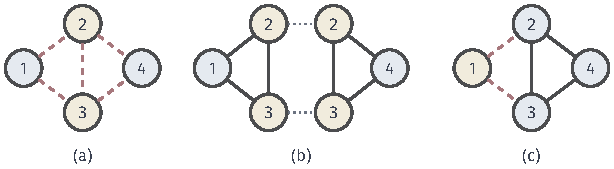
\includegraphics[width=103.9mm]{figures/01-basic-mathematics/04-graphs/tikz/c2-separator-blocks/figure.pdf}
  \caption{基于分隔集的分块。黄色顶点为候选删除集，红色虚线为随之删去的边。(a)贯穿四点图删除$S=\{2,3\}$后剩下两个分量$\{1\}$与$\{4\}$；(b)把$S$加回各侧得到两个局部块，两块中的$2,3$是同一批原顶点（点线相连），边$\{2,3\}$被两块共同引用；(c)删除$\{1\}$后余下三角形仍然连通，没有形成拆分。}
  \label{fig:graph-trav-separator-blocks}
\end{figure}

\subsection{算法分析}
\label{sec:graph-trav-blocks-interfaces}

\paragraph{正确性}
屏蔽$S$后的分量编号就是在$\mathcal G-S$上执行算法~\ref{alg:graph-trav-components}：读到屏蔽邻居不进入，等于删去了与$S$关联的边。由第~\ref{sec:graph-trav-components-forest}小节的分析，得到的$C_1,\ldots,C_r$恰是$\mathcal G-S$的连通分量，按$r$作出的判断也就正确。

局部块保存了原图的全部边。原图的一条边有三种可能：两端都在某个$C_j$中，或一端在$C_j$、一端在$S$中，这两种边都属于$\mathcal B_j$；两端都在$S$中，这样的边属于每一个块。由于不同分量之间没有边，不存在第四种情况。所以原图的全部信息都保存在这些块中，块与块之间只通过$S$发生联系。

块与块之间的联系落在接口顶点上，而各块中的接口顶点是同一批原顶点，不是可以各自独立变化的副本。若以后要给顶点赋值，同一个接口顶点在各块中必须取相同的值；若块中记录了边的数据，$S$内部的边被多个块同时看到，汇总时不能重复计数。因此算法第四步只记录接口顶点和接口边的引用，而不是把原图的一部分真正复制几份后各自修改。

\paragraph{复杂度}
屏蔽$S$并计算余图分量需要$O(n+m)$时间，输出局部块的存储则要另计。各块顶点数之和为
\[
\sum_{j=1}^{r}(|C_j|+|S|)=(n-|S|)+r|S|,
\]
接口顶点被重复列出$r$次；$S$内部的边也在每个块中出现一次。$r$和$|S|$都较小时，这部分额外存储可以忽略；接口很大或块很多时，共享引用就更为必要。

\paragraph{适用范围}
以上计算回答的是“这个给定的$S$是否拆开了图”，用$O(n+m)$时间就能完成。它不回答“最小的拆分集合是什么”。若想通过检验来找最小的分隔集，就要逐个尝试候选集合：大小为$k$的候选集有$\binom{n}{k}$个，每个都要做一次连通分量计算，规模稍大就无法承受。寻找小的分隔集需要另外的方法，它们不是一次连通标记能自动给出的。

即使找到了小的接口，也只说明块与块之间的联系少，并不说明每个块内部简单。例如两个各有$100$个顶点的完全图只共用一个顶点，删除这个顶点就把图拆成两侧，接口大小为$1$，可每个局部块仍是一个$100$个顶点的完全图。

分块的收益取决于后续计算在块内需要做什么。第~\ref{part:graph-dynamic-programming}部分会看到，当计算由许多只涉及少数顶点的局部项组成时，固定接口上的取值后各块可以分别处理，这时接口大小直接决定中间表的规模；第~\ref{chap:general-graph-dp-construction}章再把一次分块推广为多层的树分解。

\section{顶点标记与结构比较}
\label{sec:graph-wl-refinement}

第~\ref{sec:graph-isomorphism}节把两个图同构定义为存在保持邻接的顶点双射，并指出顶点数、边数、度分布等必要条件一般不足以判定同构，而直接尝试所有$n!$个双射又不可行。一种折中的办法是给每个顶点一个标记，反复根据“自己是什么、邻居都是什么”更新标记，使结构上不同的顶点逐渐得到不同的标记。这些标记不依赖顶点的编号，可以用来比较两个图，但它并不能区分所有不同构的图。

\subsection{问题与思路}
\label{sec:graph-trav-neighborhood-labels}

输入是一个无向图，顶点可以带有属性，也可以没有。我们要给每个顶点算出一个标记，满足两条要求：第一，标记只由图的结构（以及属性）决定，与顶点怎样编号无关，同构的图中对应的顶点得到相同的标记；第二，结构上不同的顶点尽可能得到不同的标记。有了这样的标记，比较两个图时就可以统计各种标记出现的次数：若次数不同，两图一定不同构。

无属性的图里，顶点一开始没有任何可区分的信息，可以给所有顶点同一个初始标记；带属性的图则可以把属性作为初始标记。

第一步自然的区分是看邻居个数，即度数：三点路径$1\text{--}2\text{--}3$中，两个端点各有一个邻居，中点有两个邻居，于是端点与中点被区分开。更进一步，不只数邻居有几个，还要看邻居分别属于哪一类、每类有几个。这样，“有两个端点邻居的顶点”和“有一个端点邻居、一个中点邻居的顶点”也能被区分。把这一步反复做下去，每做一次，顶点看到的范围就向外扩大一圈邻居。

\paragraph{多重集合}
记录“邻居都属于哪些类、各几个”，普通集合不行：两个邻居都是$A$类时，集合$\{A,A\}$就是$\{A\}$，丢失了次数。

按顶点编号排出邻居标记的序列也不行：同一个顶点的邻居换一种编号，序列的次序就变了，而我们要的信息不应依赖编号。合适的对象是\term{多重集合}（multiset）：它像集合一样不计次序，又像序列一样记录每个元素出现的次数。

用双花括号表示多重集合，例如$\{\!\{A,A,B\}\!\}$含两个$A$、一个$B$，它不等于$\{\!\{A,B\}\!\}$，但等于$\{\!\{A,B,A\}\!\}$。实际比较两个多重集合时，可以先把元素排序，再逐项比较。

把顶点自己的当前标记与邻居标记的多重集合放在一起，称为该顶点在第$t$轮的签名：
\[
\sigma_i^{(t)}=\Bigl(c_i^{(t)},\ \{\!\{c_j^{(t)}:j\in N(i)\}\!\}\Bigr).
\]
签名完全由图的结构和当前标记决定，与顶点编号无关。签名相同的顶点给同一个新标记，不同的给不同的新标记。比较两个图时，两图必须使用同一种初始标记规则，并且把签名翻译成新标记时使用同一本“字典”：同一个签名在两个图中必须得到同一个新标记。否则即使两图结构相同，标记的名称也可能对不上。

同样出于第一条要求，不能为了“容易区分”而给每个顶点附上唯一的编号作为初始标记。那样所有顶点一开始就互不相同，比较的就不再是无属性图的结构，而是“编号也必须对应”的另一个问题。只有当属性本身是图的数据、并随顶点重编号一起移动时，才把它作为初始标记，这时比较的是带属性的图。

\subsection{算法实现}
\label{sec:graph-trav-wl-algorithm}

把上一小节的思路写成精确的更新规则，就是下面的定义。

\begin{definition}[1-WL标记细化]
\label{def:graph-trav-wl-refinement}
给定无向图$\mathcal G=(V,E)$与初始标记$c_i^{(0)}$，对$t=0,1,2,\ldots$同步计算
\begin{equation}
c_i^{(t+1)}=\operatorname{enc}\bigl(\sigma_i^{(t)}\bigr)
=\operatorname{enc}\Bigl(c_i^{(t)},\ \{\!\{c_j^{(t)}:j\in N(i)\}\!\}\Bigr),
\qquad i\in V,
\label{eq:graph-trav-wl-update}
\end{equation}
其中$\operatorname{enc}$是单射，即不同的签名映为不同的新标记。这一过程称为一维Weisfeiler--Leman标记细化（1-WL），也称\term{颜色细化}（color refinement）。第$t$轮的标记把$V$划分为若干类，记为$\mathcal P^{(t)}$。
\end{definition}

算法维护三项状态：
\begin{itemize}
  \item 当前标记$c_i^{(t)}$：每个顶点一个，初始时取同一个值，带属性时取顶点属性；
  \item 字典：把已经出现过的签名翻译为标记，初始为空；
  \item 当前划分$\mathcal P^{(t)}$：由当前标记把顶点分成的类，只用于判断何时停止。
\end{itemize}

每一轮依次做三件事：
\begin{itemize}
  \item 计算签名：对每个顶点$i$读出自己的标记和全部邻居的标记，把邻居标记排序成多重集合，得到$\sigma_i^{(t)}$。
  \item 分配新标记：对每个签名查字典，已有就用对应的标记，没有就分配一个新标记并记入字典。全部顶点的新标记都算完后，才统一替换旧标记。
  \item 判断停止：比较新划分$\mathcal P^{(t+1)}$与$\mathcal P^{(t)}$，相同就停止并输出当前标记，否则进入下一轮。
\end{itemize}

统一替换是为了让第$t+1$轮的所有签名都只读取第$t$轮的标记。若边算边替换，后处理的顶点会读到一部分新标记、一部分旧标记，结果就依赖处理次序，从而依赖编号。

$\operatorname{enc}$的单射要求由字典保证；实际程序常用哈希函数把签名压缩成整数，而不同签名可能碰巧得到相同的哈希值，所以应当比较完整的签名，或用字典给每个新出现的签名分配一个新整数，不能只凭哈希值判定两个签名相等。

标记的名称每一轮都可能换新，我们关心的却是顶点被分成了哪些类，所以停止的判断看划分而不看标记本身；这一规则的合理性在下一小节证明。

\paragraph{执行过程}
图~\ref{fig:graph-trav-wl-path}从三点路径$1\text{--}2\text{--}3$开始，初始标记全为$A$。第$0$轮的签名为：端点$1,3$是$(A,\{\!\{A\}\!\})$，中点$2$是$(A,\{\!\{A,A\}\!\})$。两种签名不同，分别编码为$B$与$C$，得到$c^{(1)}=(B,C,B)$，划分为$\{1,3\}$、$\{2\}$。第$1$轮的签名为：端点是$(B,\{\!\{C\}\!\})$，中点是$(C,\{\!\{B,B\}\!\})$，编码为$D$与$E$，得到$c^{(2)}=(D,E,D)$。标记的名称换了，但划分仍是$\{1,3\}$、$\{2\}$，与上一轮相同，细化到此停止。

\begin{figure}[!htb]
  \centering
  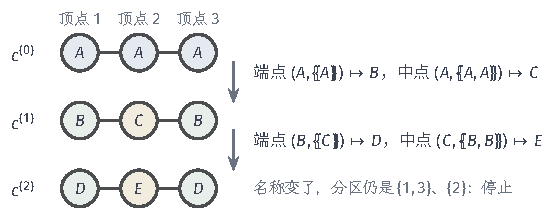
\includegraphics[width=94.0mm]{figures/01-basic-mathematics/04-graphs/tikz/c2-wl-path-refinement/figure.pdf}
  \caption{三点路径上的1-WL标记细化。每行是一轮标记，颜色表示所属的类；右侧是由签名得到新标记的编码。第一轮把端点与中点分开；第二轮标记名称改变，但划分仍为$\{1,3\}$、$\{2\}$，细化停止。}
  \label{fig:graph-trav-wl-path}
\end{figure}

\subsection{算法分析}
\label{sec:graph-trav-wl-analysis}

\paragraph{停止性}
下面的引理说明划分只会越来越细，一旦某轮没有变化，以后也不会再变；因此按划分停止是合理的，算法一定结束。

\begin{lemma}[1-WL的单调性与停止]
\label{lem:graph-trav-wl-refine}
对定义~\ref{def:graph-trav-wl-refinement}中的划分：（1）$\mathcal P^{(t+1)}$是$\mathcal P^{(t)}$的细分，即第$t+1$轮同类的顶点在第$t$轮也同类；（2）若$\mathcal P^{(t+1)}=\mathcal P^{(t)}$，则以后各轮划分都不再改变；（3）至多$n-1$轮严格细分后，划分就停止变化。
\end{lemma}

\begin{proof}
（1）若$c_i^{(t+1)}=c_j^{(t+1)}$，由$\operatorname{enc}$是单射得$\sigma_i^{(t)}=\sigma_j^{(t)}$，签名的第一个分量相等，即$c_i^{(t)}=c_j^{(t)}$。

（2）两轮划分相同，意味着存在标记之间的一一对应$\varphi$，使得对每个顶点$c_i^{(t+1)}=\varphi(c_i^{(t)})$。把$\varphi$作用到签名的每个分量上，得到$\sigma_i^{(t+1)}=\bigl(\varphi(c_i^{(t)}),\{\!\{\varphi(c_j^{(t)}):j\in N(i)\}\!\}\bigr)$。$\varphi$是一一对应，所以$\sigma_i^{(t+1)}=\sigma_k^{(t+1)}$当且仅当$\sigma_i^{(t)}=\sigma_k^{(t)}$，即$c_i^{(t+2)}=c_k^{(t+2)}$当且仅当$c_i^{(t+1)}=c_k^{(t+1)}$。因此$\mathcal P^{(t+2)}=\mathcal P^{(t+1)}$，依此类推。

（3）每次严格细分至少使类的个数加一，类的个数从至少$1$开始、不超过$n$，所以严格细分至多$n-1$次。由（2），第一次没有变化之后就再也不会变化。
\end{proof}

\paragraph{对编号的不变性}
问题的第一条要求是标记与编号无关。设$\pi$是从$\mathcal G_1$到$\mathcal G_2$的同构，且初始标记满足$c_{\pi(i)}^{(0)}=c_i^{(0)}$（无属性时所有初始标记相同，自然满足；有属性时同构本来就要求保持属性），两图共用一本字典。$\pi$把$i$的邻居一一映为$\pi(i)$的邻居，对轮数归纳可得$\sigma_{\pi(i)}^{(t)}=\sigma_i^{(t)}$，于是$c_{\pi(i)}^{(t+1)}=c_i^{(t+1)}$。特别地，对同一个图重新编号顶点（用第~\ref{sec:graph-isomorphism}节的置换表示），各顶点的标记随之移动，每种标记出现的次数不变：1-WL的结果不依赖编号，也不依赖图的画法。

\paragraph{复杂度}
每一轮要为每个顶点读取全部邻居的标记，共$O(n+m)$次读取；把顶点$i$的邻居标记排序成多重集合的规范形式需要$O(d_i\log d_i)$时间；再把全部签名排序或查字典以分配新标记。一轮的总代价为$O((n+m)\log n)$量级。由引理~\ref{lem:graph-trav-wl-refine}，至多$n$轮就能确认划分稳定（最后一轮用于确认没有变化），所以总时间不超过$O(n(n+m)\log n)$。实际图上细化往往在少数几轮内稳定，总开销远小于这个上界。

\subsection{同构检验及其局限}
\label{sec:graph-trav-wl-power}

要用1-WL比较图$\mathcal G_1$与$\mathcal G_2$，把两图放在一起看成一个不交并，用同一个初始标记规则和同一本字典同步细化，然后在每一轮分别统计两图中每种标记出现的次数。这种比较方法称为\term{一维Weisfeiler--Leman检验}（1-dimensional Weisfeiler--Leman test）。若某一轮两图的计数不同，就可以断定两图不同构；若计数在细化稳定前始终相同，只能说这一方法没有区分它们。前一结论的依据是上一小节的不变性：同构的两图在每一轮都有相同的标记计数。

例如，四个顶点的路径与四个顶点的星形都有$4$个顶点、$3$条边。初始标记全为$A$时，第一轮路径得到两个“一个邻居”的端点和两个“两个邻居”的内点，星形得到三个“一个邻居”的叶和一个“三个邻居”的中心，计数不同，两图不同构。这一轮区分的其实就是度分布，更多轮次则会区分邻居的度、邻居的邻居的度，等等。

\paragraph{局限}
1-WL的判别能力是有限的。图~\ref{fig:graph-trav-wl-limitation}中，六个顶点的环与两个不相连的三角形都有$6$个顶点、$6$条边，每个顶点的度都是$2$。

初始标记全为$A$时，每个顶点的签名都是$(A,\{\!\{A,A\}\!\})$，所有顶点得到同一个新标记；下一轮又是同样的情形。标记从第一轮起就稳定为一类，两图的计数始终相同，1-WL无法区分它们。可是它们并不同构：六环是连通的，而两个三角形构成两个连通分量。用第~\ref{sec:graph-trav-components-forest}小节的方法数一下连通分量，就能立刻把它们分开。

\begin{figure}[!htb]
  \centering
  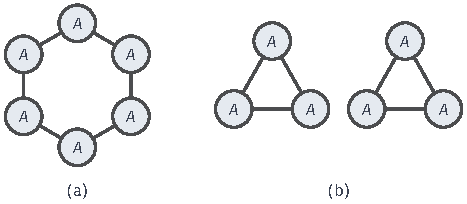
\includegraphics[width=79.5mm]{figures/01-basic-mathematics/04-graphs/tikz/c2-wl-cycle-triangles/figure.pdf}
  \caption{1-WL的局限。(a)六顶点环与(b)两个不相连的三角形初始标记全为$A$；每个顶点在每一轮都看到两个同类邻居，签名恒为$(A,\{\!\{A,A\}\!\})$，两图各轮的标记计数完全相同。两图分量数不同，并不同构。}
  \label{fig:graph-trav-wl-limitation}
\end{figure}

这个例子说明了1-WL的本质：每个顶点只能看到以自己为中心、逐轮向外扩大的邻域中“各类邻居有几个”，而六环和三角形上的每个顶点，无论看多少轮，看到的局部情形都一样。连通分量数这种整体性质，局部的计数无法反映。

因此1-WL计数不同可以作为不同构的证据，计数相同则不能作为同构的证明。实践中常把它与分量数、环长等其他检验结合使用；要确认同构，仍需给出一个实际的保持邻接的双射并逐边核对。

\section{本章小结}
\label{sec:graph-traversal-summary}

本章的出发点是：第~\ref{chap:graph-objects}章定义的可达、分量、无环、分隔和同构，怎样在一张实际的图上算出来，而不去逐条列举路径。回答的共同方式是沿邻接表有组织地访问顶点，用少量状态记住已经知道的东西，而不去枚举路径或双射。表~\ref{tab:graph-trav-summary}对照了本章各方法所维护的状态、输出和计算时间。

\begin{table*}[!htb]
  \centering
  \small
  \begin{tabular}{@{}llll@{}}
    \toprule
    方法 & 维护的状态 & 输出 & 时间 \\
    \midrule
    广度优先遍历 & 队列、距离、父指针 & 最少边数与一条最短路线 & $O(n+m)$ \\
    深度优先遍历 & 三色状态、栈帧、时刻 & 发现次序、完成次序、回边 & $O(n+m)$ \\
    分量编号 & 外层扫描、分量号 & 连通分量、生成森林 & $O(n+m)$ \\
    并查集 & 父指针树、集合大小 & 加边过程中的分量代表 & 每次$O(\log n)$ \\
    Kosaraju算法 & 完成次序、反向图 & 强连通分量、缩点图 & $O(n+m)$ \\
    Kahn算法 & 当前入度、零入度队列 & 拓扑序或有环报告 & $O(n+m)$ \\
    分隔集分块 & 屏蔽标记、分量号 & 余图分量、局部块 & $O(n+m)$ \\
    1-WL细化 & 各轮标记、签名字典 & 稳定划分、标记计数 & 每轮$O((n+m)\log n)$ \\
    \bottomrule
  \end{tabular}
  \caption{本章方法维护的状态、输出与时间。时间均以邻接表存储计，$n$为顶点数，$m$为边数或弧数。}
  \label{tab:graph-trav-summary}
\end{table*}

这些输出回答的是不同的问题。广度优先遍历的层数回答“离起点最少几步”，深度优先遍历的完成次序回答“谁的后续全部探完”，它在无环图上给出拓扑序，在一般有向图上把强连通分量按缩点图的先后分离出来。并查集的代表元回答“在已加入的边下是否连通”，分隔集分块回答“删去给定接口后图分成几侧”，1-WL的标记回答“局部邻域在计数意义下是否一样”。

同一张图上，这些量可以同时计算，但不能互相替代：深度优先的父路径不是最短路线，发现次序不是拓扑序，并查集的父指针不是原图的边，1-WL计数相同也不是同构的证明。

判断一个算法的输出是否正确，标准是看它是否满足相应的结构条件，而不只是看算法是否停止。广度优先遍历的父路径应恰有$d(v)$条边；生成森林应有$n-c$条边且无环；拓扑序应使每条弧从前指向后；有环报告应附带一个可以逐弧核对的环；强连通分量在第二遍中不应越过已标记的分量；分块检验应报告余图实际有几个分量。各节的定理正是把这些条件与算法的状态联系起来的依据。

本章得到的可达区域、生成森林和依赖次序，都只描述了“能否连接、按什么次序”，没有比较不同路线或不同边集的代价：广度优先遍历只数边数，生成森林只保证连通。第~\ref{part:graph-combinatorial-optimization}部分在这些结构的基础上引入边上的数值，研究最短路、最小生成树、最大流、匹配与指派和最小费用流。本章的工具在那里继续使用：拓扑序用于第~\ref{chap:shortest-paths}章有向无环图上的最短路递推，并查集用于第~\ref{chap:minimum-spanning-tree}章的Kruskal算法，广度优先遍历用于第~\ref{chap:max-flow-min-cut}章在残量网络中寻找弧数最少的增广路径。

第~\ref{sec:graph-separator-blocks}节的接口思想则在第~\ref{part:graph-dynamic-programming}部分展开：固定接口上的取值后，各局部块上的计算可以分别进行，再沿接口汇总。


